\RequirePackage{etoolbox}
\csdef{input@path}{%
 {sty/}% cls, sty files
 {img/}% eps files
}%
\csgdef{bibdir}{bib/}% bst, bib files

\documentclass[ba]{imsart}
%
\pubyear{0000}
\volume{00}
\issue{0}
\doi{0000}
\firstpage{1}
\lastpage{1}

%
\usepackage{amsthm}
\usepackage{amsmath}
\usepackage{natbib}
\usepackage[colorlinks,citecolor=blue,urlcolor=blue,filecolor=blue,backref=page]{hyperref}
\usepackage{graphicx}

\startlocaldefs

\endlocaldefs


%\usepackage{fullpage,amsmath}% mathtools}
%\usepackage{setspace}
\usepackage{graphicx, psfrag, amsfonts, float}
\usepackage{natbib}
\usepackage{amsthm}
\usepackage{multirow}
\usepackage{hhline}
%\usepackage{color}
%\usepackage[position=t,singlelinecheck=off]{subcaption}
%\usepackage{caption, setspace}
%\usepackage[position=t,singlelinecheck=off]{subfigure}
 \pdfminorversion=4
\usepackage{rotating}
\def\bgam{\mbox{\boldmath $\gamma$}}
\def\bth{\mbox{\boldmath $\theta$}}
\def\bbeta{\mbox{\boldmath $\beta$}}
\def\blam{\mbox{\boldmath $\lambda$}}
\def\bmu{\mbox{\boldmath $\mu$}}

\newcommand{\bx}{\mbox{\boldmath $x$}}
\newcommand{\bu}{\mbox{\boldmath $u$}}
\newcommand{\bc}{\mbox{\boldmath $c$}}
\newcommand{\bs}{\mbox{\boldmath $s$}}
\newcommand{\by}{\mbox{\boldmath $y$}}
\newcommand{\bz}{\mbox{\boldmath $z$}}
\newcommand{\bv}{\mbox{\boldmath $v$}}
\newcommand{\bb}{\mbox{\boldmath $b$}}
\newcommand{\bzero}{\mbox{\boldmath $0$}}
\newcommand{\thstarj}{\mbox{$\theta^\star_j$}}
\newcommand{\bths}{\mbox{$\btheta^\star$}}
\newcommand{\pkg}[1]{{\fontseries{b}\selectfont #1}} 

\newcommand{\ud}{\mathrm{d}}
\newcommand{\uI}{\mathrm{I}}
\newcommand{\uP}{\mathrm{P}}
\newcommand{\up}{\mathrm{p}}
\newcommand{\mb}{\mathbf}
\newcommand{\mc}{\mathcal}


\newcommand{\Bern}{\mbox{Bern}}
\newcommand{\Nor}{\mbox{N}}
\newcommand{\Ga}{\mbox{Gamma}}
\newcommand{\Dir}{\mbox{Dir}}
\newcommand{\Ber}{\mbox{Ber}}
\newcommand{\Be}{\mbox{Be}}
\newcommand{\Unif}{\mbox{Unif}}
\newcommand{\Binom}{\mbox{Bin}}
\newcommand{\IG}{\mbox{IG}}

\newcommand{\Xs}{X^\star}
\newcommand{\Lc}{{\cal L}}


\usepackage[dvipsnames,usenames]{color}
\newcommand{\yy}{\color{magenta}\it}
\newcommand{\jj}{\color{Black}\rm}
\newcommand{\yjnote}[1]{\footnote{\color{Brown}\rm #1 \color{Black}}}
\newtheorem{theorem}{Theorem}[section]
\newtheorem{definition}[theorem]{\bf Definition}
\newtheorem{lemma}[theorem]{\bf Lemma}
\newtheorem{corollary}[theorem]{\bf Corollary}
\newtheorem{proposition}[theorem]{\bf Proposition}
\newtheorem{assumption}[theorem]{\bf Assumption}
\newtheorem{example}[theorem]{\bf Example}
\newtheorem{remark}[theorem]{\bf Remark}


\newcommand{\iid}{\stackrel{iid}{\sim}}
\newcommand{\indep}{\stackrel{indep}{\sim}}

\doublespacing
\setlength{\textwidth}{6 in}

% commands for for editing
\usepackage{color}
\usepackage{ulem} % \sout
\newcommand{\red}[1]{{\color{red}#1}}
\newcommand{\blue}[1]{{\color{blue}#1}}
\newcommand{\brown}[1]{{\color{brown}#1}}
\newcommand{\green}[1]{{\color{green}#1}}
\newcommand{\magenta}[1]{{\color{magenta}#1}}
\newcommand{\response}[1]{{\color{blue}#1}}
\DeclareMathOperator*{\argmin}{\arg\!\min}
\graphicspath{{figures/}{figs/}}


\makeatletter
\newcommand{\labitem}[2]{%
\def\@itemlabel{\textbf{#1}{.}}
\item
\def\@currentlabel{#1}\label{#2}}
\makeatother


%  Points to handle in preparing the manuscript
%
%  1.  Out of sample evaluation of the model.  We should go with trimmed mean log-likelihood (trimming the cases
%       that contribute least to log-likelihood).  Justification for the trimming mentioned in a sentence
%       here, to be more carefully and completely done in separate work (with Yoonsuh).  
%
%  3.  Add quite a number of references to Section 2.  This is where we should catch the old work
%      that conditions on the sample mean and proceeds through asymptotic approximation, Peter 
%      Hoff's work on ranks, Holmes and Walker's work, and ABC.  New text needs to accompany the
%      references, making clear what the other work does and how ours differs.  The new text should
%      be quite brief.  
%
%  4.  A big question.  Should we try to add any asymptotic theory?  A Section 3.4?  See next comment.  
%      My vote is "no".  
%
%  5.  Page limitations.  A goal for the entire manuscript is 30 pages.  Current length is 34+, spilling
%      onto page 35.  But, additions will include the abstract (1/2 page or so), conclusions (1 page or 
%      so), more references (another half page?), and more writing scattered throughout.  Redoing
%      figures (two to drop) and tables will save a modest amount of space.   I propose that we 
%      hold off on adding new content until we see how long the paper is.  Also, new content along
%      the lines of point 4 would mean that we have to prove/use existing results to show the truth
%      of whatever we claim!  
%
%  6.  Confirm with Nationwide that they are okay with our using their data and that they are comfortable
%       with the descriptions we have in the paper.  
%
%  7.  Fit the hierarchical model, conditioning on the robust summaries at each leaf in the model.  
%
%  9.  A hedge on computations?  There are examples (pathological in some senses) for which a basic
%      MCMC based on the complete data works, but where conditioning on a poorly chosen T(y) leads
%      to a reducible Markov chain.  I don't think this happens when the support of y is the same for all
%      \theta (it may be that mutual absolute continuity of all distributions for y|\theta is needed, though
%      definitions of "support" vary somewhat).  I think we can ignore this here, but an example could go
%      into the dissertation.  (one sentence now included to hint at this).  



%  To be added
%
%  1.  Abstract.  
%
%  2.  Conclusions.  To be written later.  I will take a pass at them once a few results are filled in for
%       the data analysis.  
%

%  John.  
%  See notes in red throughout.  The overarching goal is to move the manuscript toward completion.  
%  To do so means filling in details to get them taken care of.  Big batches are (i) references, (ii) 
%  deciding on notation for the estimator (b to replace beta?), (iii) verifying that the theorems have the
%  right conditions, (iv) patching figures, (v) adding material for the examples, and (vi) deciding whether
%  the figure and text on the last two pages is needed.  
%  If you want to add comments for us, pick a color other than red and add them in that color.  

%  Yoon.  
%  A check on the theorems would be great.  No need, I think, to dig out the paper by Miao and Ben Israel
%  as that part of the math is fine (I'll check to make sure that all conditions for our use of the theorems have
%  been stated in the Corollary).  Once more details are in place, proof reading and adjustment.  

%\newpage

\begin{document}

\begin{frontmatter}
\title{Bayesian Restricted Likelihood Methods: Conditioning on Insufficient Statistics in Bayesian Regression\thanksref{T1}}
\runtitle{Bayesian Restricted Likelihood Methods}
\thankstext{T1}{This research has been supported by Nationwide Insurance Company and by the NSF under grant numbers DMS-1007682 and DMS-1209194.  The views in this paper are not necessarily those of Nationwide Insurance or the NSF.} 

\begin{aug}
\author{\fnms{John R.} \snm{Lewis}\thanksref{addr1,m1}\ead[label=e1]{lewis.865@buckeyemail.osu.edu}}, 
\author{\fnms{Steven N.} \snm{MacEachern}\thanksref{addr1,m1}\ead[label=e2]{snm@stat.osu.edu}}, 
\and  
\author{\fnms{Yoonkyung} \snm{Lee}\thanksref{addr1,m1}\ead[label=e3]{yklee@stat.osu.edu}} \\
%{\small \it Department of Statistics, The Ohio State University, Columbus, Ohio 43210}\\
%{\small lewis.865@osu.edu, snm@stat.osu.edu and yklee@stat.osu.edu}
\runauthor{J. Lewis et al}

\address[addr1]{Department of Statistics, The Ohio State University, Columbus, Ohio 43210 
    \printead{e1}, % print email address of "e1"
    \printead*{e2},
    \printead*{e3}
}
\end{aug}


\begin{abstract}
Bayesian methods have proven themselves to be successful across a wide
range of scientific problems and have many well-documented advantages
over competing methods. However, these methods run into difficulties
for two major and prevalent classes of problems: handling data sets
with outliers and dealing with model misspecification. We outline the
drawbacks of previous solutions to both of these problems and propose a new method as an
alternative.  When working with the new method, the data is summarized
through a set of insufficient statistics, targeting inferential quantities of interest, and the prior
distribution is updated with the summary statistics rather than the complete
data.  By careful choice of conditioning statistics, we
retain the main benefits of Bayesian methods while reducing the
sensitivity of the analysis to features of the data not captured by
the conditioning statistics. For reducing sensitivity to outliers,
classical robust estimators (e.g., M-estimators) are natural choices
for conditioning statistics. %With these choices, the method can be thought of as a blend of classical robust estimation and Bayesian methods. 
A major contribution of this work is the development of a data 
augmented Markov chain Monte Carlo (MCMC) algorithm
for the linear model and a large class of
summary statistics. We demonstrate the method on simulated and real data sets containing outliers and subject to model
misspecification. Success is manifested in better predictive
performance for data points of interest as compared to competing
methods.
\end{abstract}
%\noindent KEYWORDS: Approximate Bayesian computation, Markov chain
%Monte Carlo, M-estimation, Robust regression.

%\begin{keyword}[class=MSC]
%\kwd[Primary ]{60K35}
%\kwd{60K35}
%\kwd[; secondary ]{60K35}
%\end{keyword}

\begin{keyword}
%\kwd{Approximate Bayesian computation}
\kwd{Markov chain Monte Carlo}
\kwd{M-estimation}
\kwd{Robust regression}
\end{keyword}

\end{frontmatter}

\section{Introduction}
Bayesian methods have provided successful solutions to a wide range of scientific problems, with their value
having been demonstrated both empirically and theoretically.  Bayesian inference relies on a model consisting of three elements:  the prior distribution, the loss function, and the likelihood or sampling density.  While formal optimality of Bayesian methods is unquestioned if one accepts the validity of all three of these elements, a healthy skepticism encourages us to question each of them.  Concern about the prior distribution has been addressed through the development of techniques for subjective elicitation \citep{garthwaite2005, ohagan2006} and objective Bayesian methods \citep{berger2006}.  Concern about the loss function is reflected in, for example, the extensive literature on Bayesian hypothesis tests \citep{kass1995}.  The focus of this work is the development of techniques to handle imperfections in the likelihood $f(\by|\bth) = L(\bth|\by)$. Concern for imperfections in the likelihood are reflected in work considering minimally informative likelihoods \citep{yuan1999minimally}, sensitivities of inferences to perturbations in the model \citep{zhu2011}, the specification of a class of models and the use of Bayesian model averaging over the class \citep{clyde2004}, and considerations of such averaging when the specified class may not contain the so-called true data generating model \citep{bernardo2000, clyde2013, clarke2013Complete}.   In practice, the imperfections in a proposed likelihood often show themselves through the presence of outliers -- cases not reflecting the phenomenon under study. There are three main solutions to Bayesian outlier-handling.  The first is to replace the basic sampling density with a mixture model which includes one component for the ``good'' data and a second component for the ``bad'' data.  With this approach, the good component of the sampling density is used for prediction of future good data.  The second approach replaces the
basic sampling density with a thick-tailed density in an attempt to discount outliers, yielding techniques that often provide solid estimates of the center of the distribution but do not easily translate to predictive densities for further good data.  The third approach fits a flexible (typically nonparametric) model to  the data, producing a Bayesian version of a density estimate for both good and bad data.  In recent development, inference is made through the use of robust inference functions \citep{lee2014}.  

These traditional strategies  all have their drawbacks.  The outlier-generating processes 
may be transitory in nature, constantly shifting as the source of bad data changes.  This prevents us from appealing to large-sample arguments to claim that, with enough data, we can nail down a model for both good and bad data combined.  Instead of attempting to model both good and bad data, we propose a novel strategy for handling outliers. In a nutshell, we begin with a complete model  as if all of the data are good. Rather than driving the move from prior to posterior  by the full likelihood, we use only the likelihood driven by a few summary statistics which typically target inferential quantities
of interest.  We call this likelihood a restricted likelihood because conditioning is done on a restricted set of data; the set which satisfies the observed summary statistics. This restricted likelihood leads to a formal update of the prior distribution based on the sampling density of the summary statistics. 

%\response{The advantages and disadvantages of the method are detailed throughout the paper using simulated data and real data. One conceptual advantage is that inferences and predictions are less sensitive to features of the data not captured by the conditioning statistics. Choosing statistics targeting main features of interest allows for more targeted inference on these features. The analysis can help to better understand other features, such as outliers, not capture by the conditioning statistics.} 
%\response{The examples in the paper suggest advantages in situations where outliers are concern and there is significant prior information for the non-outlying portion of the model that is not outweighed by the data. The main disadvantage over traditional robust estimate techniques are mainly computational. In Section ~\ref{BayesLinMod} we detail a data-augmented MCMC algorithm to fit the models proposed in this paper. This requires an additional computational step for each iteration of the chain. Details of the additional burden are given and one must weigh the advantages of these methods with this additional burden. Since it is typically that the restricted likelihood posterior converges to the same expected value as the conditioning statistics as the sample size grows, it may not be practical to implement our method in all situations.}
\response{The advantages and disadvantages of the method are detailed throughout the paper using simulated and real data. One conceptual advantage of our method is that inferences and predictions are less sensitive to features of the data not captured by
the conditioning statistics than are methods based on the complete likelihood. Choosing statistics targeting the main features of interest allows for inference that focuses on these features. The analysis can help to better understand other features which may not be captured by the conditioning statistics, such as outliers.} 

\response{The examples in the paper provide a Bayesian analog of classical robust estimators.  The main disadvantage of our methods relative to the classical estimators is computational.  In Section~\ref{BayesLinMod} we detail a data-augmentation MCMC algorithm to fit the models proposed in this paper.  The advantages are those of Bayesian methods.  As is standard for Bayes-classical comparisons, the Bayesian method requires greater computational effort while providing better inference.  As a referee notes, asymptotically, the Bayesian and classical parameter estimates are often very close and have the same limiting posterior variance / sampling variance.  In situations where asymptotic approximation suffices, there is no need to use the computational techniques developed in this paper.}

The remainder of the paper is as follows: Section~\ref{restrictedlikelihood} introduces the Bayesian restricted likelihood, provides context with previous work, and demonstrates some advantages of the methods on simple examples. Section~\ref{BayesLinMod} details an MCMC algorithm to apply the method to Bayesian linear models. This computational strategy is a major contribution to the work, providing an approach to apply the method on realistic examples. Many of the the technical proofs are in the Appendix \ref{sec:appendix} with \texttt{R} code available from the authors. Sections \ref{simData} and \ref{RealData} illustrate the method with simulated data and a real insurance industry data set containing many outliers with a novel twist on model evaluation. A discussion (Section~\ref{Conclusions}) provides some final commentary on the new method. \response{ An R package \texttt{brlm} to implement our methods is available at \texttt{github.com/jrlewi/brlm}. Additionally all data and code for the examples in this paper are available at \texttt{https://github.com/jrlewi/brlm\char`_paper/revision\char`_2}.}

\section{Restricted Likelihood}
\label{restrictedlikelihood}
%\textcolor{blue}{Tried to make more concise. Commented out section describing the further examples related to randomized experiments, contingency tables, and meta-analysis. }

\subsection{Examples}
To describe the use of the restricted likelihood, 
we begin with a pair of simple examples for the one-sample problem.  For both, the model takes the data $\by=(y_1,\ldots,y_n)$ to be a random sample
of size $n$ from a continuous distribution indexed by a parameter
vector $\bth$, with pdf $f(y| \bth)$.  The standard, or full,
likelihood is $L(\bth | \by) = \prod_{i=1}^n f(y_i | \bth)$.  

The first example considers the case where a known subset of the data are known to be 
bad in the sense of not informing us about $\bth$.  This case mimics the setting where outliers are identified and discarded before doing a formal analysis.  Without loss of generality, we label the good cases $1$ through $n-k$ and the bad cases $n-k+1$ through $n$.  The relevant likelihood to be used to move from prior distribution to posterior distribution is clearly $L(\bth | y_1, \ldots, y_{n-k}) = \prod_{i=1}^{n-k} f(y_i | \bth)$.  For an equivalent analysis, we rewrite the full likelihood as the product of two pieces:
\begin{eqnarray}
\label{OutlyingCases}
L(\bth | \by)  
= \left( \prod_{i=1}^{n-k} f(y_i | \bth) \right) \left( \prod_{i=n-k+1}^{n} f(y_i | \bth) \right), 
\end{eqnarray}
where the second factor may not actually depend on $\bth$. We wish to keep the first factor and drop the second for better inference on $\bth$.

The second example involves deliberate censoring of small and large observations. This is
sometimes done as a precursor to the analysis of reaction time experiments  \citep[e.g.,][]{ratcliff1993} where very small and large reaction times are physiologically implausible;  explained by either anticipation or lack of attention of the subject.  
With lower and upper censoring times at $t_1$ and $t_2$, the post-censoring sampling distribution is of mixed form, with masses $F(t_1|\bth)$ at $t_1$ and $1-F(t_2|\bth)$ at $t_2$,
and density $f(y | \bth)$ for $y \in (t_1, t_2)$.  We adjust the original data $y_i$,
producing $c(y_i)$ by defining $c(y_i)= t_1$ if $y_i \leq t_1$, $c(y_i)=t_2$ 
if $y_i \geq t_2$, and $c(y_i)=y_i$ otherwise.  
The adjusted update is performed with $L(\bth |c(\by))$.  
Letting $g(t_1|\bth) = F(t_1|\bth)$,
$g(t_2 | \bth) = 1 - F(t_2|\bth)$, and $g(y|\bth)=f(y|\bth)$ for
$y \in (t_1, t_2)$, we may rewrite the full 
likelihood as the product of two pieces
\begin{eqnarray}
\label{Censoring} 
L(\bth  | \by) =  \left( \prod_{i=1}^n g(c(y_i)  | \bth) \right) \left( \prod_{i=1}^n f(y_i|\bth,c(y_i)). \right) ,  
\end{eqnarray}

$\prod_{i=1}^n f(y_i|\bth,c(y_i))$ is the likelihood of the data conditioned on parameters and the summary statistic $c(\cdot)$ and recovers the piece of the full likelihood not in $ \prod_{i=1}^n g(c(y_i)  | \bth)$. Only the first part is retained in the analysis. Several more examples are detailed in \cite{lewis2014}.



%Further examples abound. In a completely randomized experimental design, we randomize %our 
%experimental units to treatment conditions and then ignore the details of the observed randomization \citep{dean1999}; 
%in work with contingency tables,  
%we collapse categories with small counts, coarsening the scale of %our 
%data \citep{agresti2002}; in meta-analysis, we ignore the individual patient-level data and instead
%work with estimated effects from the studies \citep{orourke2007}.  
%Further examples are described in \cite{lewis2014}. 
\subsection{Generalization}

To generalize the approach in \eqref{OutlyingCases} and
\eqref{Censoring}, %, and these other settings,
we write the full likelihood in two pieces with a conditioning statistic $T(\by)$, as indicated below:
\begin{eqnarray}
\label{FullLikelihood}
L(\bth | \by)  
& = & f(T(\by) | \bth) \,\, f(\by |\bth, T(\by)) .  
\end{eqnarray}
%Throughout the paper, we use the convention that a function is defined by its inputs. 
Here,  $f(T(\by) | \bth)$ is the conditional pdf of $T(\by)$ given $\bth$ and $f(\by |\bth, T(\by))$ is the conditional pdf of $\by$ given $\bth$ and $T(\by)$.  In the dropped case example, the conditioning statistic is $T(\by) = (y_1, \ldots, y_{n-k})$.  In 
the censoring example, the conditioning statistic is $T(\by) = (c(y_1),\ldots,c(y_n))$.  We refer to 
$f(T(\by) | \bth)$ as the restricted likelihood and $L(\bth | \by)=f(\by|\bth)$ as the full likelihood.  

Bayesian methods can make use of a restricted likelihood %in place of a complete likelihood
since $T(\by)$ is a well-defined random variable with a probability distribution indexed by $\bth$.  
This leads to the restricted likelihood posterior 
\begin{eqnarray}
\label{RestrictedPosterior}
\pi(\bth | T(\by)) & = & \frac{\pi(\bth) f(T(\by) | \bth)}{m(T(\by))} ,
\end{eqnarray}
where $m(T(\by))$ is the marginal distribution of $T(\by)$ under the prior distribution.  
Predictive statements for further (good) data rely on the model.  For another observation,
say $y_{n+1}$, we would have the predictive density 
\begin{eqnarray}
\label{RestrictedpredDist}
f(y_{n+1} | T(\by)) = \int f(y_{n+1} | \bth) \pi(\bth | T(\by))\ d\bth .  
\end{eqnarray}

\subsection{Literature review}

Our motivation for the use of summary statistics in Bayesian inference is concern about outliers or, more generally, model misspecification. Specifically, the likelihood is not specified correctly and concentrating on using well chosen parts of the data can help improve the analysis \citep[e.g.,][]{wong2004}. Direct use of restricted likelihood for this reason appears in many areas of the literature.  For example, the use of rank likelihoods is discussed by \cite{savage1969}, \cite{pettitt1983, pettitt1982}, and more recently by \cite{hoff2013}.  
\cite{lewis2012} make use of order statistics and robust estimators as choices for $T(\by)$ in the location-scale setting. 
Asymptotic properties of restricted posteriors are studied by \cite{doksum1990}, \cite{clarke1995}, \cite{yuan2004},  and \cite{hwang2005}. The tenor of these asymptotic results is that, for a variety of conditioning statistics with non-trivial regularity conditions on prior, model, and likelihood, the
posterior distribution resembles the asymptotic sampling distribution of the conditioning statistic.  

Restricted likelihoods have also been used as practical approximations to a full likelihood. For example, \cite{pratt1965} appeals to heuristic arguments regarding approximate sufficiency to justify the use of the restricted likelihood of the sample mean and standard deviation. Approximate sufficiency is also appealed to in the use of Approximate Bayesian Computation (ABC), which is related to our method.  
ABC is a collection of posterior approximation methods which has recently experienced success in applications to epidemiology, genetics, and quality control \citep[see, for example,][]{tavare1997, pritchard1999,  marjoram2003, fearnhead2012}. Interest typically lies in the full data posterior and ABC is used for computational convenience as an approximation.  Consequently, effort is made to choose an approximately sufficient $T(\by)$ and update to the ABC posterior by using the likelihood $L(\bth| \mathcal{B}(\by))$, where $\mathcal{B}(\by)=\{\by^{*}|\rho(T(\by),T(\by^{*})) \leq \epsilon\}$, $\rho$ is a metric, and $\epsilon$ is a tolerance level. This is the likelihood conditioned on the collection of data sets that result in a $T(\cdot)$ within $\epsilon$ of the observed $T(\by)$. %Hence, we can see that, as in our method, conditioning is done on a summary of the complete data. 
With an approximately sufficient $T(\cdot)$ and a small enough $\epsilon$, heuristically  $L(\bth|\mathcal{B}(\by))\approx L(\bth|T(\by))\approx L(\bth|\by)$. Consequently, the ABC posterior approximates the full data posterior and efforts have been made to formalize what is meant by  approximate sufficiency \citep[e.g.,][]{joyce2008}. ABC is related to our method in that the conditioning is on something other than the data $\by$.  However, we specifically seek to condition on an insufficient statistic to guard against misspecification in parts of the likelihood. Additionally, we develop methods where the conditioning is exact (i.e. $\epsilon = 0$).


%ABC is related to our method in that conditioning is on something other than the complete data. Even if $T(\by)$ were exactly  sufficient in the traditional sense, a positive $\epsilon$ would result in something theoretically different from the complete data posterior (even if they are indeed approximately the same). We also mention that in ABC, $\mathcal{B}(\by)$ is not a statistic in the strict sense because it does not partition the sample space before observing data. That is, a feasible data set $\bz^{*}$ can belong to more than one `ball'  $\mathcal{B}(\cdot)$.  The method relies on conditioning on this set because in most ABC applications, approximating the complete data posterior directly is hard (or impossible) and sampling data matching the observed summary exactly is also hard (or impossible). ABC methods are a practical and useful solution in these settings. For the regression models we present, sampling new data matching the observed summary exactly is indeed possible and so we can condition exactly on the observed summary. Further, we reiterate that our motivation is different from ABC in that we do not want to condition on the complete data because we assume it contains inherent flaws which can be detrimental to inference. 

%However, the conditioning in ABC is heuristic.  For technical reasons, the calculation proceeding from $\pi(\bth)$ to $\pi(\bth)L(\bth| \mathcal{B}(\by))/\int \pi(\bth)L(\bth| \mathcal{B}(\by)) d\bth$ is not a formal conditional update.  Simply put, if an external observer told $\mathcal{B}(\by)$ can supply $T(\by)$ and vice-versa, the information contained in $\mathcal{B}(\by)$ is exactly that contained in $T(\by)$ and proper conditioning will lead to identical posterior distributions.  This is not the case with a typical implementation of ABC.  

% In a related, but distinctly different, approach which also takes advantage of summary statistics, the full data log likelihood is replaced by a loss function \citep[e.g.][]{bissiri2013} in an effort to concentrate inference only on parameters of interest. In contrast, the incomplete likelihood is formulated using a full probability model, allowing for a formal Bayesian update, while remaining robust to misspecification.

This work extends the development of Bayesian restricted likelihood by arguing that deliberate choice of an insufficient statistic $T(\by)$ guided by targeted inference is sound practice. We also expand the class of conditioning statistics for which a formal Bayesian update can be achieved.  Our methods do not rely on asymptotic properties, nor do they rely on approximate conditioning.%, \green{nor do they need to correspond to artificial censoring to create incomplete or missing data}  \citep[e.g.,][]{albert1988, hoffwakefield2013}.  
%\green{Note - fix references here hoffwakefield for asymptotic; albert for ? .}  

%The key to productive use of the restricted likelihood is the choice of $T(\by)$ and the development
%of computational strategies that allow us to truly condition on the observed $T(\by)$ and 
%fit the model in formal Bayesian fashion.  In this work, we focus
%on robustness, and natural choices of $T(\by)$ for the one-sample problem include a set of middling order statistics, a trimmed
%mean, or a classical robust estimator of location and/or scale.  
%We have previously implemented several of these methods and have found them to perform well \citep[][]{lewis2012}. Versions most extensible to the linear model include the M-estimators in the tradition of \cite{huber1964}, least median squares (LMS), and least trimmed squares (LTS). For these choices the restricted likelihood is not available in closed form, making computation of the restricted posterior a challenge. For low-dimensional statistics $T(\by)$ and parameters $\bth$, the direct computational strategies described in \cite{lewis2014} can be used to estimate the incomplete posterior conditioned on essentially any statistic.  These strategies rely on generation of complete data sets from different values of $\bth$.  
%Each complete data set leads to a statistic $T(\by)$ under $\bth$, and these generated statistics are used to estimate the density at $T(\by_{obs})$, where $\by_{obs}$ is the observed complete data. This estimate is fed into Bayes' theorem for the update from prior distribution to posterior distribution.  


%For the example in the previous section, these strategies work well.
%\textcolor{blue}{Comment out `A variety of  variance reduction techniques which exploit\dots' because it seemed too vague and a bit off topic}
%In low dimensional settings (in $T(\by)$ and $\bth$) the incomplete posterior under each of these versions (and others) can be estimated by approximating the incomplete likelihood using kernel density estimation techniques \citep[for details see][]{lewis2014}. 

%These direct sampling techniques rely on density estimation and numerical integration. Density estimation becomes difficult for high dimensional $T(\by)$ and numerical integration breaks down for high dimensional $\bth$. For these settings, an MCMC algorithm is developed in Section \ref{highDim}. Software is available from the authors for use with simultaneous M-estimators of location and scale. At the present time, further software development is required to extend beyond simultaneous M-estimators.  

%\textcolor{blue}{Added a bit about this to the discussion: Though we concentrate in this paper on applying incomplete likelihood inference for the mean of linear regression models, the computational strategies we devise in subsequent sections also allow us to apply the method to inference beyond the mean.  In particular, quantile regression falls within the framework we develop. }
%The next section develops the necessary computational strategies.  

%\subsection{Details of Examples in Section \ref{illustrations}}
%\subsubsection{Speed of Light}
%With parameters $\beta$ and $\sigma$, the full model is $\beta\sim N(23.6, 2.04^{2})$, $\sigma^{2}\sim IG(5, 10)$, $y_{i}\iid N (\beta, \sigma^{2})$ for $i=1,2,\dots, n=66$ where $y_{i}$ denotes the $i^{th}$ measurement of the passage time of light. $\beta$ is interpreted as the passage time of light with
%$\sigma^{2}$ representing measurement error. Tuning parameters for the M-estimators are chosen to achieve $95\%$ efficiency under normality and for comparability, roughly $5\%$ of the residuals are trimmed for LTS.  The t-model assumes $y_{i}\iid t_{\nu} (\beta, \sigma^{2})$ with $\nu=5$. The prior on $\sigma^{2}$ is $IG(5, \frac{\nu-2}{\nu}10)$ so the prior on the variance is the same as the other models. %We note that the variance of the data under this model is $\frac{\nu}{\nu-2}\sigma^{2}$.  For comparability, it is this quantity that has the prior distribution $IG(a,b)$ given above.   \citep[for details see][]{huber2009


\subsection{Illustrative Examples}
\label{illustrations}
Before discussing computational details, the method is applied to two simple examples on well known data sets to demonstrate its effectiveness in situations where outliers are a major concern. The full model in each case fits into the Bayesian linear regression framework discussed in Section \ref{BayesLinMod}. The first example is an analysis of Simon Newcomb's 66 measurements of the passage time of light \citep{stigler1977}; two of which are significant outliers in the lower tail. The full model is a standard location-scale Bayesian model also used in \cite{lee2014}:
\begin{equation}
\beta\sim N(23.6, 2.04^{2}),\  \sigma^{2}\sim IG(5, 10), \ y_{i}\iid N (\beta, \sigma^{2}), i=1,2,\dots, n=66,
\end{equation}
where $y_{i}$ denotes the $i^{th}$ (recorded) measurement of the passage time of light. $\beta$ is interpreted as the passage time of light with the deviations $y_i - \beta$ representing measurement error.
Four versions of the restricted likelihood are fit with conditioning statistics: 1) Huber's M-estimator for location with Huber's `proposal 2'  for scale 2)  Tukey's M-estimator for location with Huber's `proposal 2'  for scale 3) LMS (least median squares) for location with associated estimator of scale and 4) LTS (least trimmed squares)  for location with associated estimator of scale. \response{Details of these estimators can be found in many places, including \citep{huber2009}. We return to the two M-estimators throughout this paper as we have found them to offer good default choices for practitioners dealing with outliers. A short review of these estimators is provided in the Supplementary Material.}  The tuning parameters for the M-estimators are chosen to achieve $95\%$ efficiency under normality \citep{huber2009} and, for comparability, roughly $5\%$ of the residuals are trimmed for LTS.  Two additional approaches to outlier handling are considered: 1) the normal distribution is replaced with a t-distribution and, 2) the normal distribution is replaced with a mixture of two normals. The t-model assumes $y_{i}\iid t_{\nu} (\beta, \sigma^{2})$ with $\nu=5$. The prior on $\sigma^{2}$ is $IG(5, \frac{\nu-2}{\nu}10)$ and ensures that the prior on the variance is the same as the other models. The mixture takes the form: $y_{i}\iid pN (\beta, \sigma^{2}) + (1-p)N(\beta, 10\sigma^{2})$ with the prior $p \sim \text{beta}(20,1)$ on the probability of belonging to the `good' component.  

The posterior of $\beta$ under each model appears in Figure \ref{fig:newcomb_post}.  The posteriors group into two batches.  The normal model and restricted likelihood with LMS do not discount the outliers and have posteriors centered at low values of $\beta$.  These posteriors are also quite diffuse.  In contrast, the t-model, mixture model, and the other restricted likelihood methods discount the outliers and have posteriors centered at higher values.  There is modest variation among these centers.  Posteriors in this second group have less dispersion than those in the first group.   
\begin{figure}[t]
\centering
{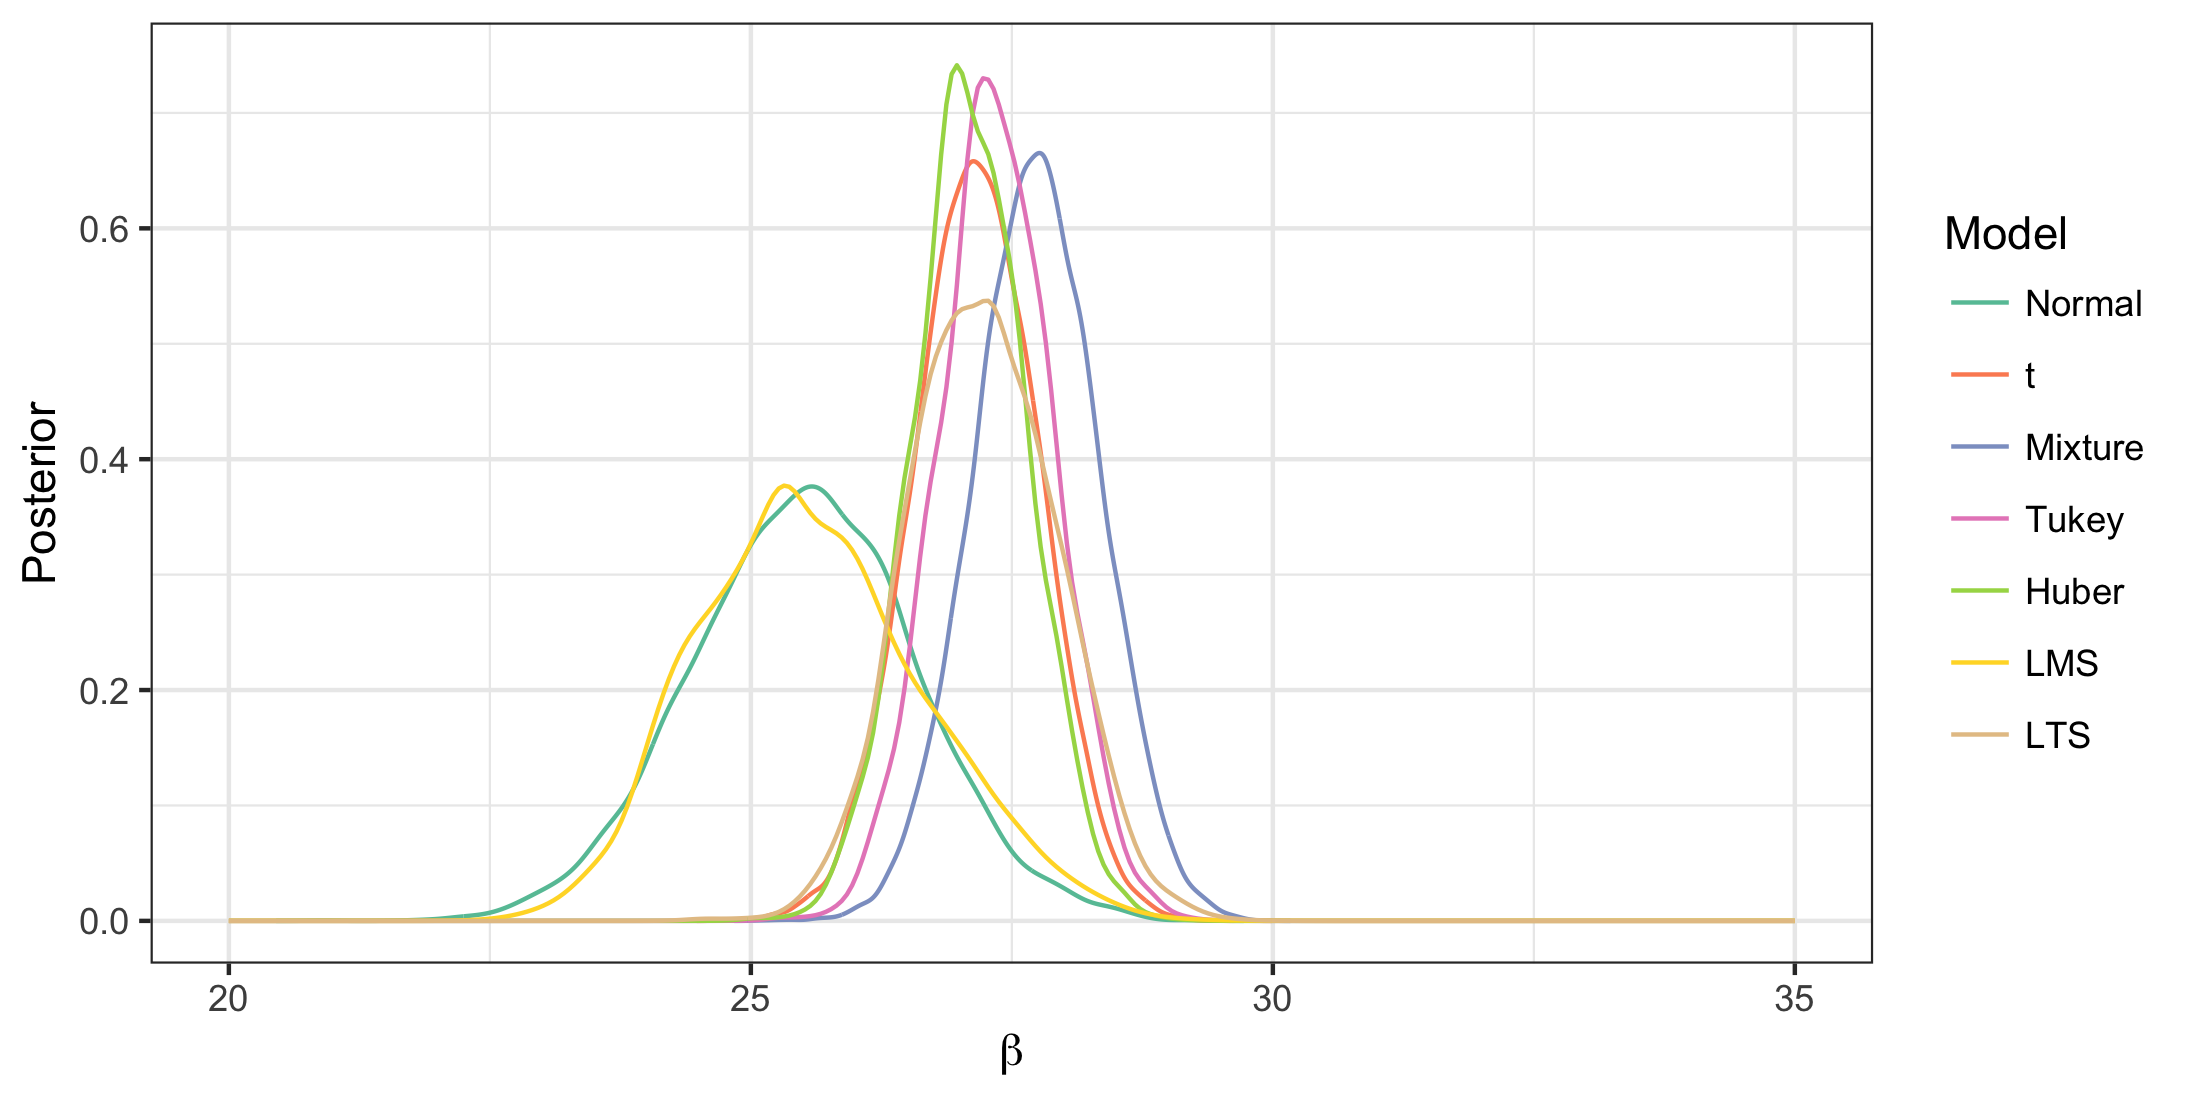
\includegraphics[width = 4in]{figs/speed_of_light_beta.png}}
{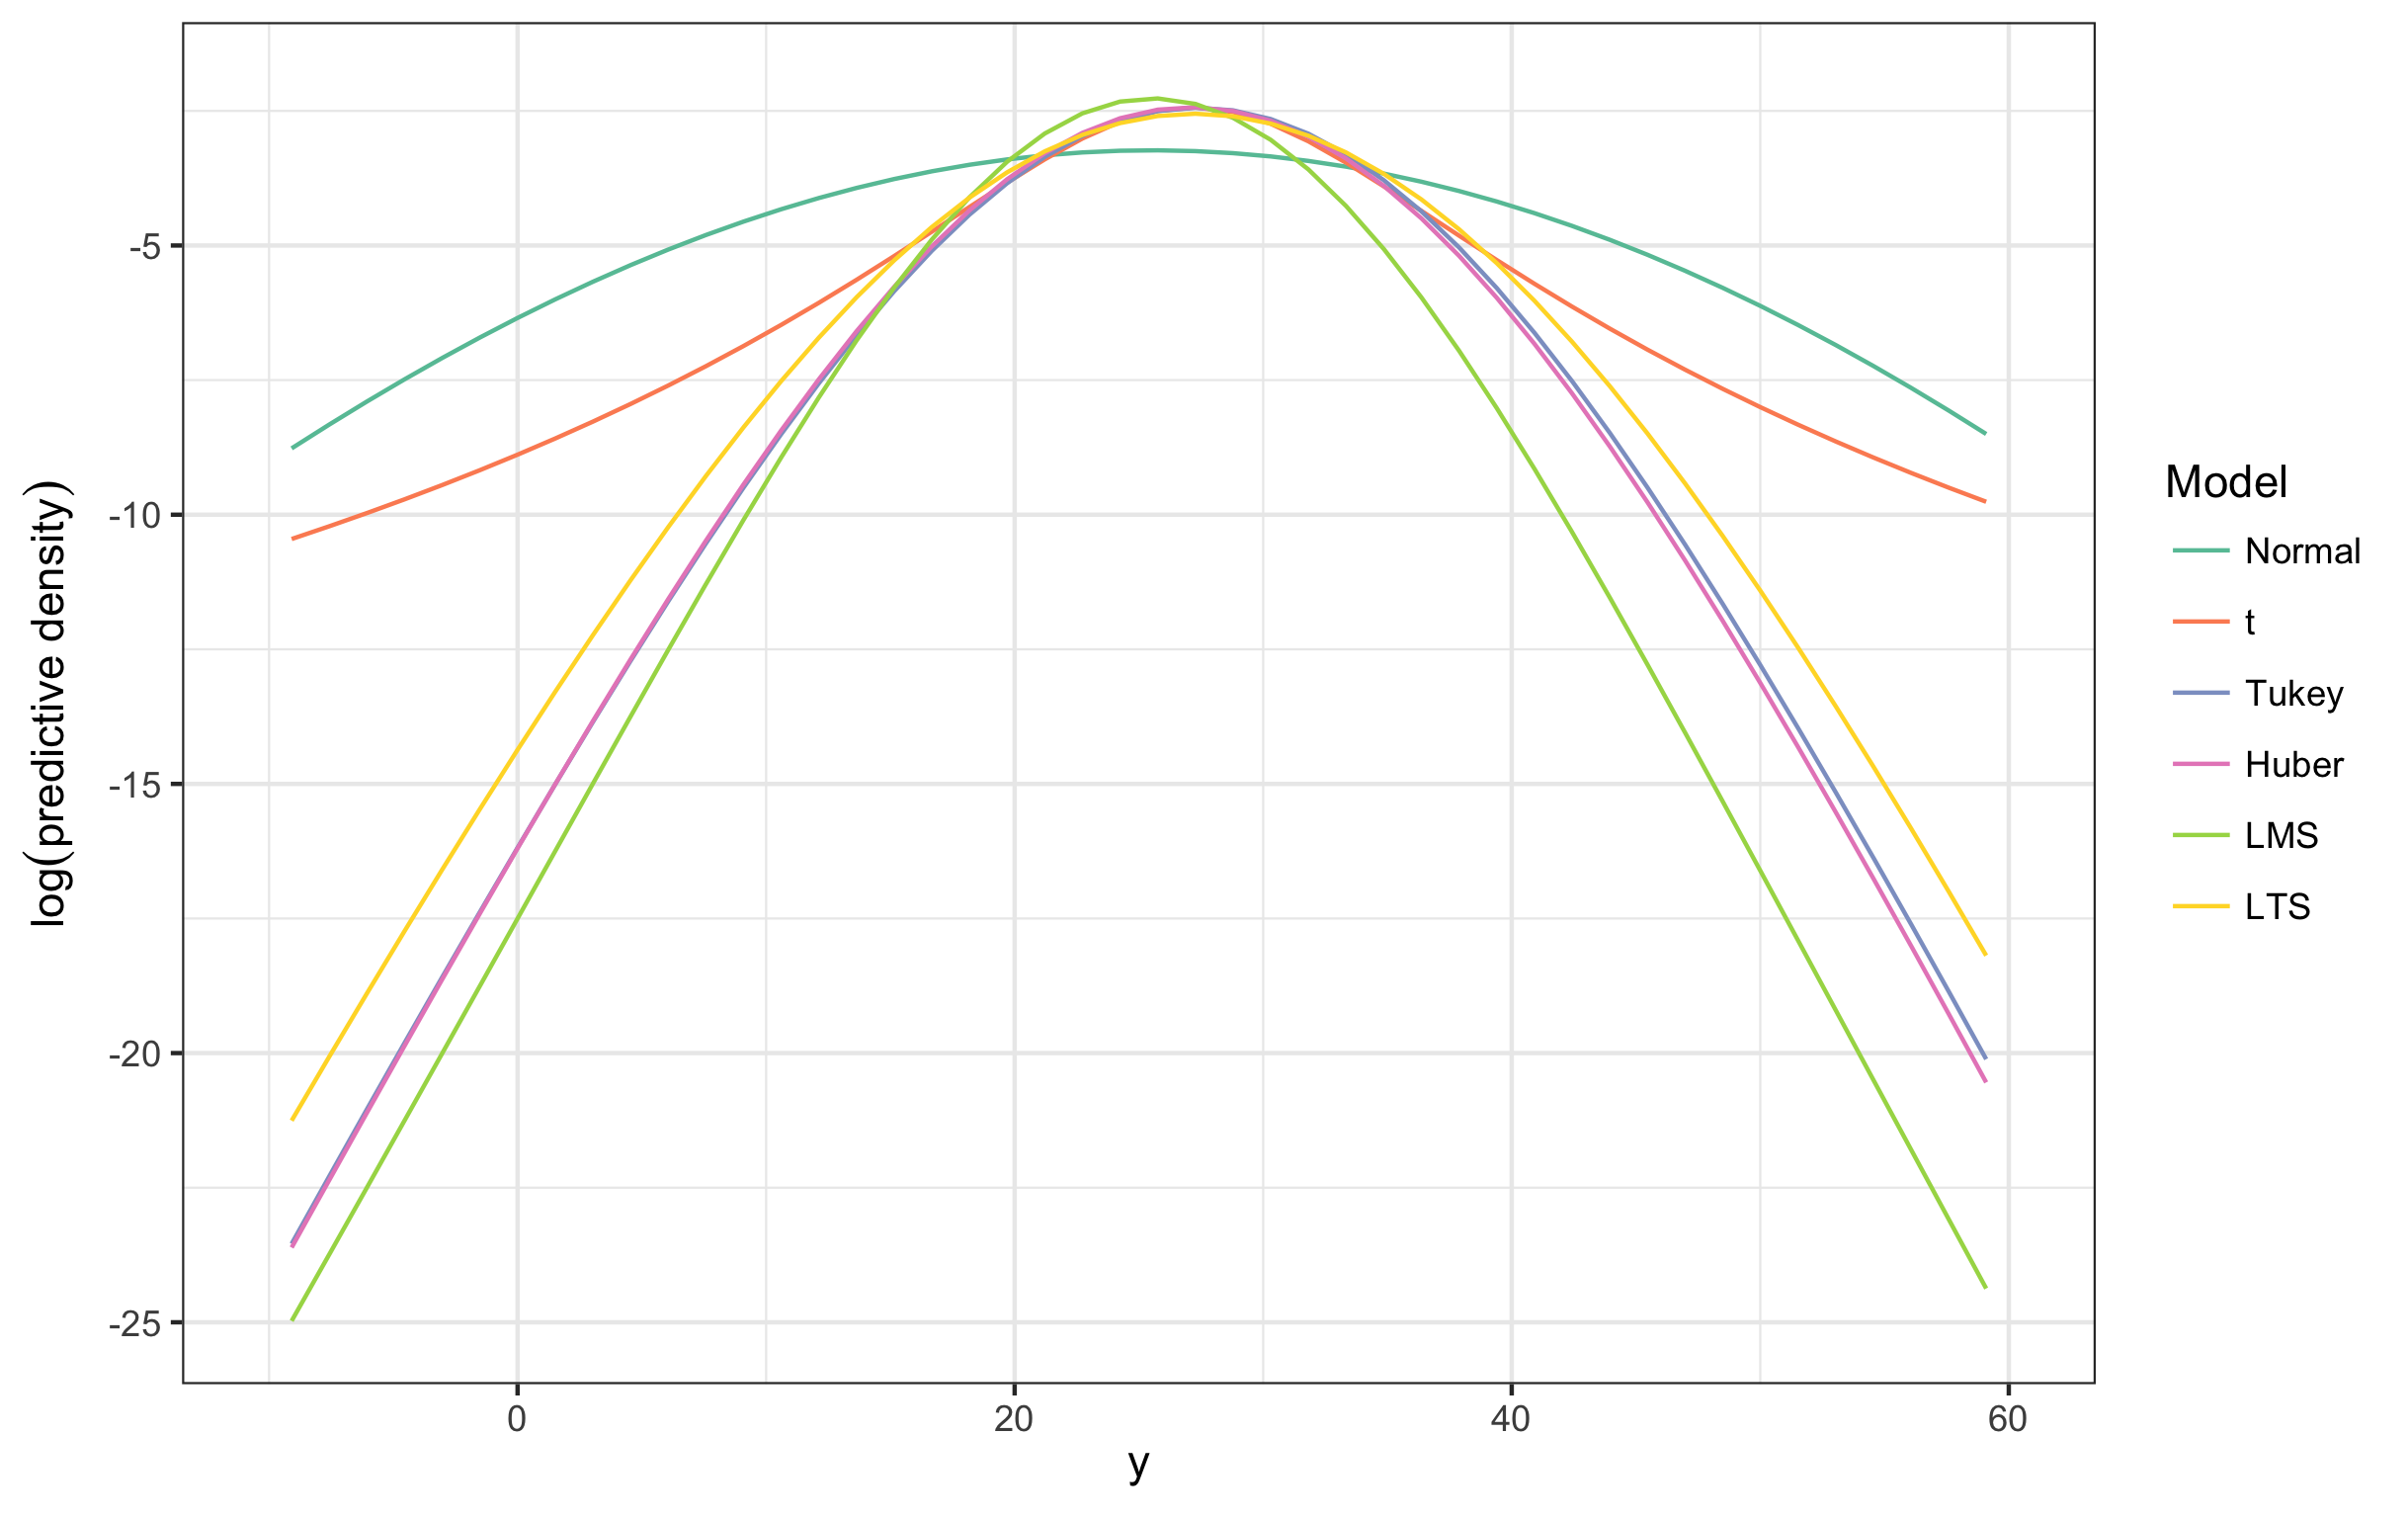
\includegraphics[width = 4in]{figs/speed_of_light_predictive.png}}
\caption{Results from the analysis of the speed of light data. Top: Posterior distributions of $\beta$ under each model. Bottom: Log posterior predictive distributions under each model. The differences in the tails are emphasized in the bottom plot. The horizontal axis is strategically labeled to help compare the centers of the distributions in each of the plots.}
\label{fig:newcomb_post}
\end{figure}
The pattern for predictive distributions differs (see bottom plot in Figure \ref{fig:newcomb_post}).  The normal and t-models have widely dispersed predictive distributions.  The other predictive distributions show much greater concentration.  The restricted likelihood fits based on M-estimators (Tukey's and Huber's) are centered appropriately and are concentrated. The restricted likelihood based on LTS and the mixture model results are also centered appropriately, but comparatively less concentrated. The LMS predictive is concentrated, but it is poorly centered.  

%Overall, we find that the restricted likelihood methods based on M-estimators provide the most attractive analysis for these data.  They provide sharp and appropriate inference for parameters ($\beta$) and for prediction. A second example on well known data is provided in the Supplementary Material.

As a second example, a data set measuring the number of telephone calls in Belgium from 1950-1973 is analyzed. The outliers in this case are due to a change in measurement units on which calls were recorded for part of the data set. Specifically, for years 1964-1969 and parts of 1963 and 1970, the length of calls in minutes were recorded rather than the number of calls \citep{rousseeuw1987}. The full model is a standard normal Bayesian linear regression:
\begin{equation}
{\boldsymbol{\beta}}\sim N_{2}(\boldsymbol{\mu}_{0}, \boldsymbol{\Sigma}_{0}),\  \sigma^{2} \sim IG(a, b),\  \by \sim N(X\boldsymbol{\beta}, \sigma^{2} I),
\end{equation}
where $\bbeta = (\beta_{0}, \beta_{1})^{\top}$, $\by$ is the vector of the logarithm of the number of calls, and $X$ is the $n\times 2$ design matrix with a vector of 1's in the first column and the year covariate in the second. \response{In reality, the model should include a different piece for the part of the data with different units. The outliers are really just a manifestation of model misspecification.} Prior parameters are fixed via a maximum likelihood fit to the first 3 data points. In particular, the prior covariance for $\bbeta$ is set to $\Sigma_{0} = g\sigma_{0}^2 (X_{p}^{\top}X_{p})^{-1}$, with $X_{p}$ the $3\times 2$ design matrix for the first $3$ data points, $g=n=21$, $\sigma_{0} = 0.03$ and $\boldsymbol{\mu}_{0} = (1.87,  0.03)^{\top}$.  This has the spirit of a unit information prior \citep{kass1995reference} but uses a design matrix for data not used in the fit. Finally $a = 2$ and $b =1$.

Four models are compared: 1) the normal theory base model 2) a two component normal mixture model, 3) a t-model, and 4) a restricted likelihood model conditioning on Tukey's M-estimator for the slope and intercept with Huber's `proposal 2'  for scale. Each model is fit to the remaining 21 data points. The normal theory model is also fit a second time after removing observations 14-21 (years 1963 - 1970). The omitted cases consist of the obvious large outliers as well as the two smaller outliers at the beginning and end of this sequence of points caused by the change in measurement units. The mixture model allows different mean regression functions and variances for each component.  Both components have the same, relatively vague priors. The probability of belonging to the first component is given a $\text{beta}(5,1)$ prior. The heavy-tailed model fixes the degrees of freedom at 5 and uses the same prior on $\bbeta$.  The prior on $\sigma^2$ is adjusted by a scale factor of $3/5$ to provide the same prior on the variance.  

The data and  $95\%$ credible bands for the posterior predictive distribution under each model are displayed in Figure \ref{fig:calls_predictive}. The normal model fit to all cases results in a very wide posterior predictive distribution due to an inflated estimate of the variance. The t-model provides a similar predictive distribution.  The pocket of outliers from 1963 to 1970 overwhelms the natural robustness of the model and leads to wide prediction bands.  The outliers, falling toward the end of the time period, lead to a relatively high slope for the regression.  In contrast, the normal theory model fit to only the good data results in a smaller slope and narrower prediction bands.  The predictive distribution under the restricted likelihood approach is much more precise and is close to that of the normal theory fit to the non-outlying cases. The two component mixture model provides similar results, where the predictive distribution is formulated using only the good component. For these data, the large outliers are easily identified as following a distinct regression, leaving the primary component of the mixture for non-outlying data.  In a more complex situation where the outlier generating mechanism is transient (i.e., ever changing and more complex than for these data), modeling the outliers is more difficult. As in classical robust estimation, the restricted likelihood approach avoids explicitly modeling the outliers. 
\begin{figure}[t]
\centering
{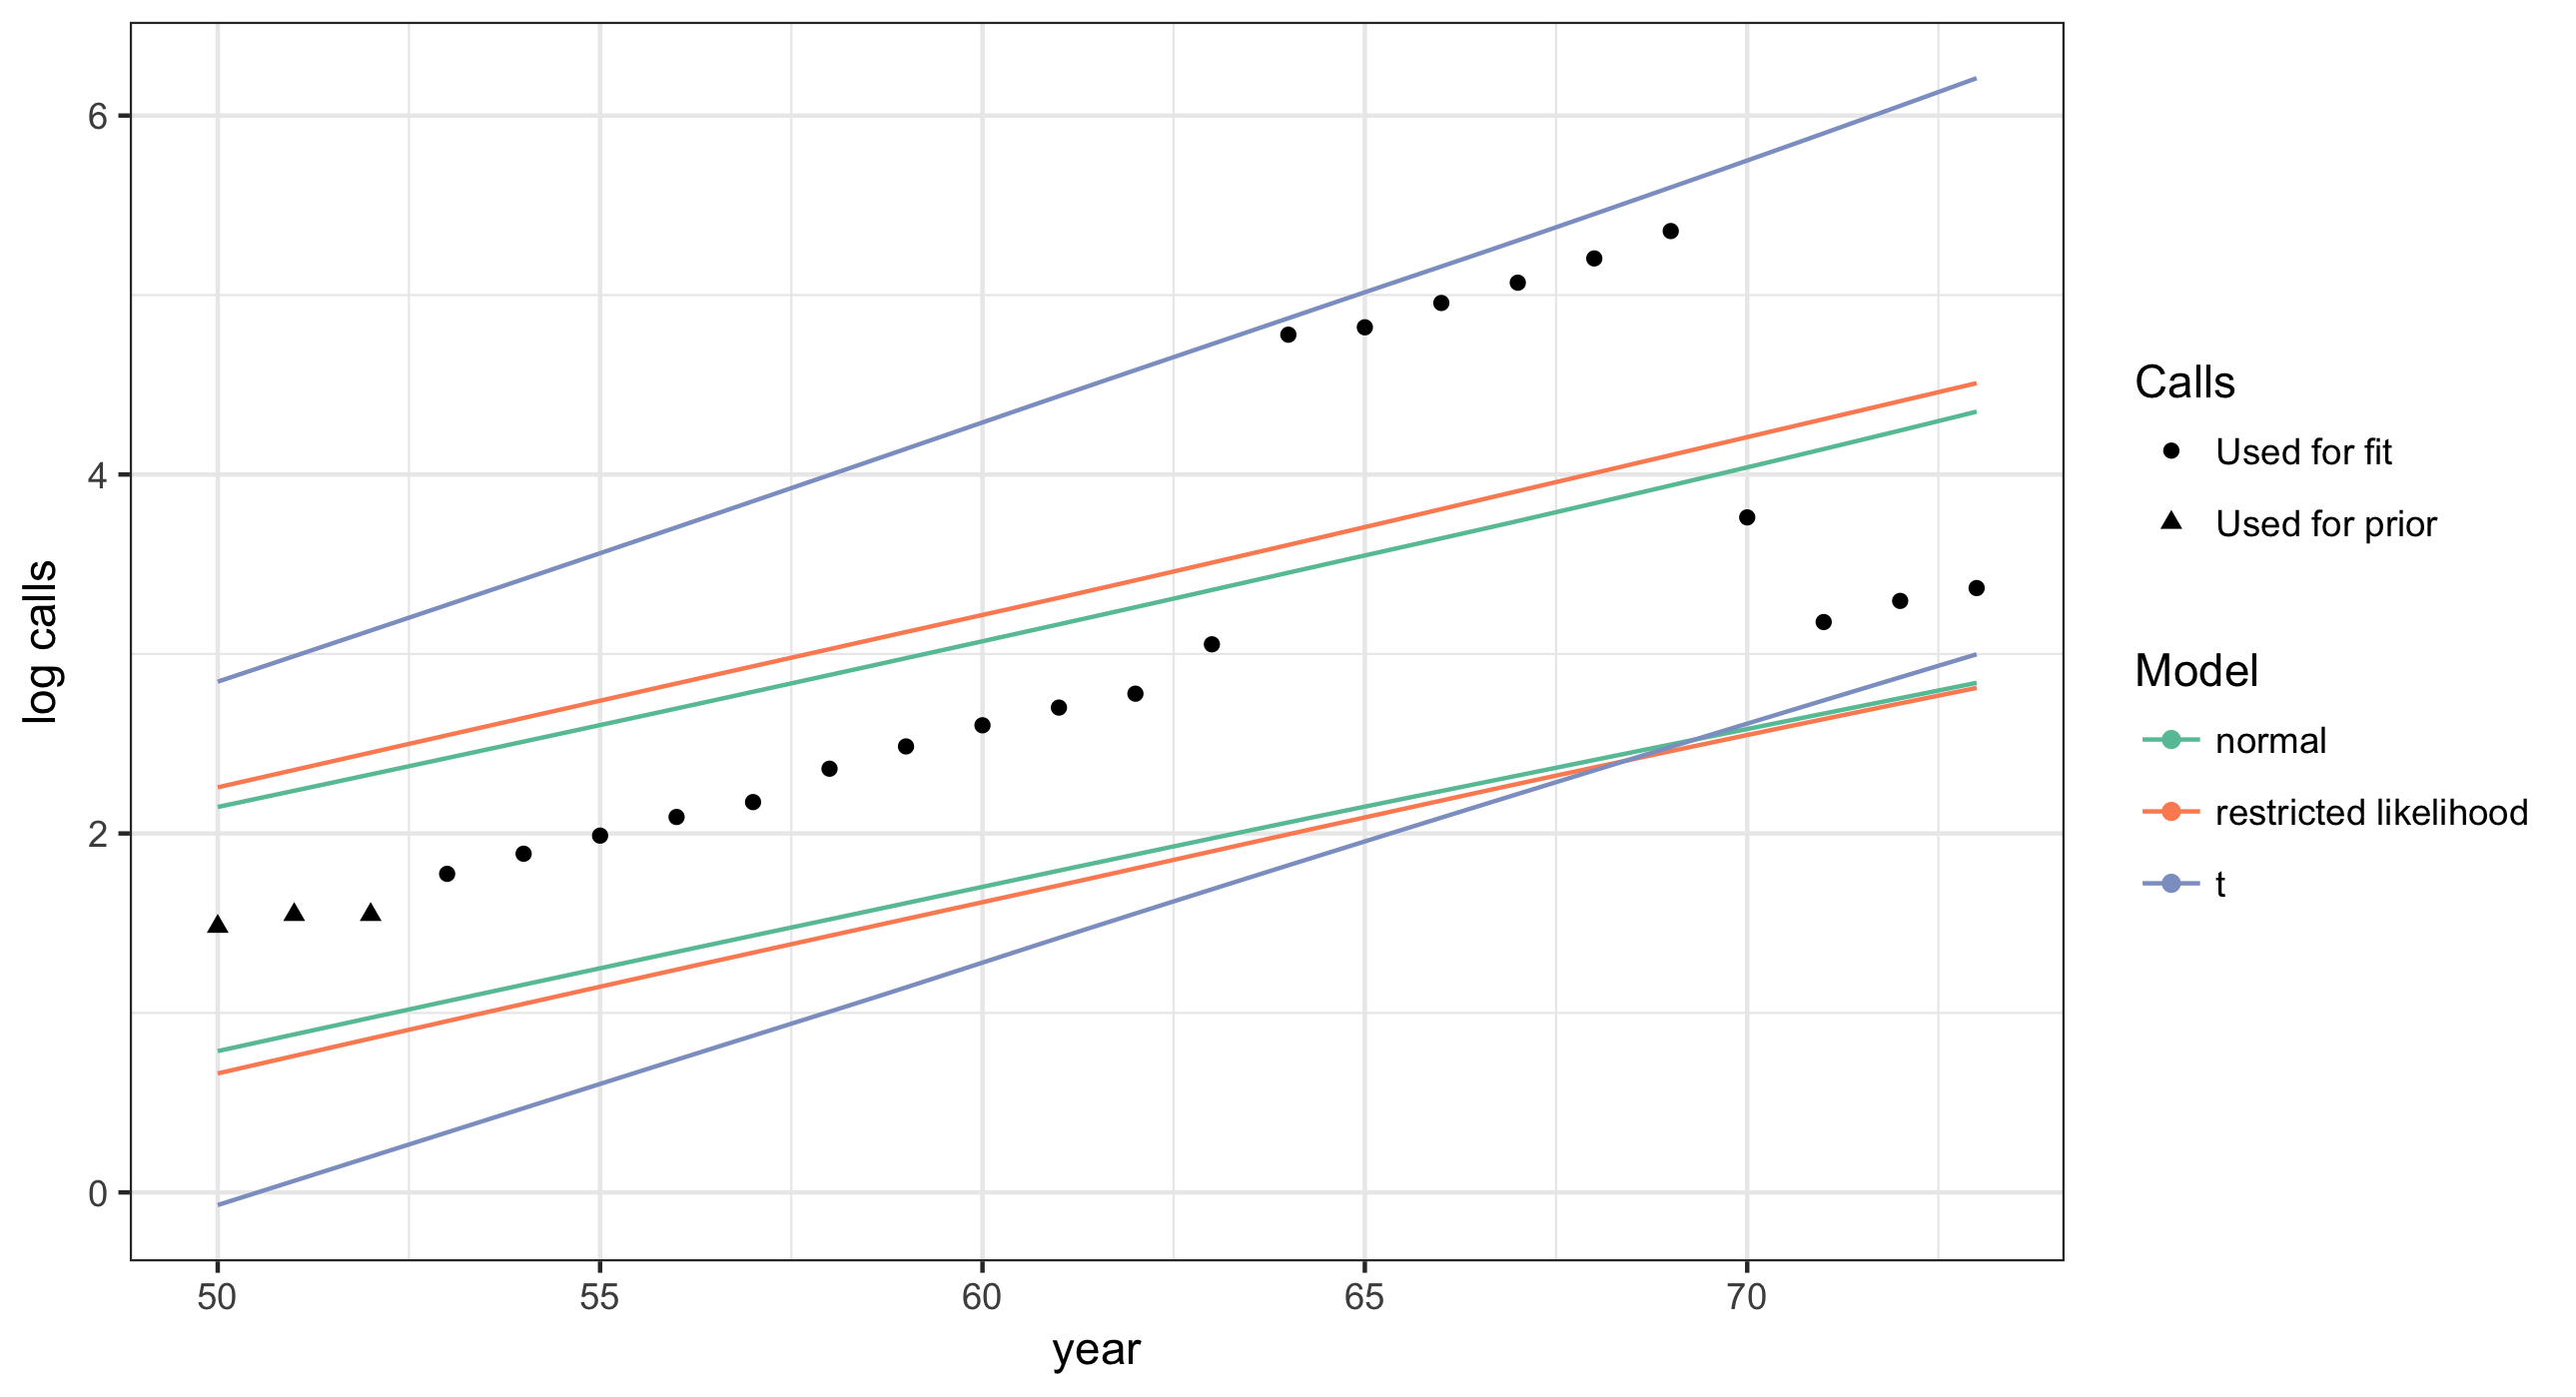
\includegraphics[width = 4in]{figs/calls_predictive.png}}
\caption{Pointwise posterior predictive intervals of log(calls) under the normal theory model fit to the non-outliers, the restricted likelihood model with Tukey's M-estimator for the slope and intercept with Huber's `proposal 2'  for scale, and a heavy-tailed t-distribution model. The first three data points were used to specify the prior with each model using the remaining 21 for fitting. The normal theory model was also fit after removing observations 14-20 (years 1963 - 1970).}
\label{fig:calls_predictive}
\end{figure}






\section{Restricted Likelihood for the Linear Model}
\label{BayesLinMod}
The simple examples in the previous section highlight the beneficial impact of a good choice of $T(\by)$ with the use of the restricted likelihood. This work focuses on robustness in linear models where natural choices include many used above:  M-estimators in the tradition of \cite{huber1964}, least median squares (LMS), and least trimmed squares (LTS). For these choices the restricted likelihood is not available in closed form, making computation of the restricted posterior a challenge. For low-dimensional statistics $T(\by)$ and parameters $\bth$, the direct computational strategies described in \cite{lewis2014} can be used to estimate the restricted posterior conditioned on essentially any statistic.  These strategies rely on estimation of the density of $f(T(\by)|\theta)$ using samples of $T(\by)$ for many values of $\bth$; a strategy which breaks down in higher dimensions. This section outlines a data augmented MCMC algorithm that can be applied to the Bayesian linear model when $T(\by)$ consists of estimates of the regression coefficients and scale parameter. 

\subsection{The Bayesian linear model}
We focus on the use of restricted likelihood for the Bayesian linear
model with a standard formulation: 
\begin{eqnarray}
\label{LinearModel}
\bth&=&(\bbeta,\sigma^2) \sim  \pi(\bth) 
\nonumber\\
y_i  & =  & x_i^\top \bbeta + \epsilon_i , \mbox{ for } i = 1, \ldots, n 
\end{eqnarray}
where $x_i$ and $\bbeta \in \mathbb{R}^p$, $\sigma^2 \in \mathbb{R}^+$, 
and the $\epsilon_i$ are independent draws from a distribution with center $0$ and scale $\sigma$. $X$ denotes the design matrix whose rows are  $x_i^\top$. For the restricted likelihood model,  conditioning statistics are assumed to be of the form $T(\by) = (\bb(X, \by), s(X, \by))$ where $\bb(X, \by)= (b_1(X,\by), \dots,b_p(X,\by))^\top\in \mathbb R^{p}$ is an estimator for the regression coefficients and $s(X, \by)\in \{0\} \cup {\mathbb R}^+$ is an estimator of the scale. Throughout, observed data and summary statistic is denoted by $\by_{obs}$ and $T(\by_{obs})=(\bb(X, \by_{obs}), s(X, \by_{obs}))$, respectively. 
Several conditions are imposed on the model and statistic to ensure validity of the MCMC algorithm:
\begin{itemize}
\labitem{C1}{fullRank} The $n \times p$ design matrix, $X$, whose $i^{th}$ row is $x_i^\top$, 
is of full column rank.  
\labitem{C2}{supReal} The $\epsilon_i$ are a random sample from some distribution which has a density with 
respect to Lebesgue measure on the real line and for which the support is the real line.  
\labitem{C3}{asb}$\bb(X,\by)$ is almost surely continuous and differentiable with respect to $\by$.  
\labitem{C4}{as} $s(X,\by)$ is almost surely positive, continuous, and differentiable with respect to $\by$.  
\labitem{C5}{regEq} $\bb(X,\by+X\bv)=\bb(X,\by)+\bv \ \ \text{for  all}\ \bv\in\mathbb{R}^p$. 
\labitem{C6}{scaleEqReg} $\bb(X,a\by)=a\bb(X,\by)\ \ \ \text{for all constants } a$.  
\labitem{C7}{regIn} $s(X,\by+X\bv)=s(X,\by) \ \ \text{for all}\ \bv\in\mathbb{R}^p$.  
\labitem{C8}{scaleEq2Reg} $s(X, a\by)=|a|s(X,\by) \ \ \text{for all constants } a$.  
\end{itemize}
Properties \ref{regEq} and \ref{scaleEqReg} of $\bb$ are called
\textit{regression} and \textit{scale equivariance},
respectively.  Properties \ref{regIn} and \ref{scaleEq2Reg} of $s$ are called \textit{regression invariance}
and \textit{scale equivariance}. 
Many estimators satisfy the above properties, including several traditional simultaneous M-estimators \citep{huber2009, maronna2006} for which the \texttt{R} package \texttt{brlm} (\texttt{github.com/jrlewi/brlm}) is available to implement the MCMC described here. 
%\response{These M-estimators satisfy \ref{asb}-\ref{as} since they are optimizers of (almost surely) continuous and differentiable objective functions. Constraints  \ref{regEq}-\ref{scaleEq2Reg} are often satisfied by location and scale estimators but should be checked on a case by case basis.}
\response{These M-estimators satisfy \ref{asb} and \ref{as} since they are optimizers of continuous and differentiable objective functions. Constraints \ref{regEq}-\ref{scaleEq2Reg} are often satisfied by location and scale estimators but should be checked on a case by case basis.}  
More software development is required to extend the MCMC implementation beyond the M-estimators discussed here. The current version of the \texttt{R} package also implements the direct methods described in \cite{lewis2014}. These methods are effective in lower dimensional problems and were used in both examples in Section \ref{illustrations}.

%The strategy described in the previous paragraph extends to full-blown regression models.  Robust regression methods lead naturally to a conditioning statistic in the form of a classical M-estimator for $\bbeta$
%and a companion estimator for $\sigma$.  We denote the resulting estimator which involves the covariates through
%the design matrix and the response 
%as $T(\by) = (\bb(X,\by), s(X,\by))$, with $\bb(X,\by) = (b_1(X,\by), \cdots,
%b_p(X,\by))^\top$.  Simultaneous M-estimators have a number of standard properties \ref{asb}-\ref{scaleEq2Reg} which
%prove useful in the sequel \citep{huber2009, maronna2006}.  
%\begin{itemize}
%\labitem{C3}{asb}$\bb(X,\by)$ is almost surely continuous and differentiable with respect to $\by$.  
%\labitem{C4}{as} $s(X,\by)$ is almost surely positive, continuous, and differentiable with respect to $\by$.  
%\labitem{C5}{regEq} $\bb(X,\by+X\bv)=\bb(X,\by)+\bv \ \ \text{for  all}\ \bv\in\mathbb{R}^p$. 
%\labitem{C6}{scaleEqReg} $\bb(X,a\by)=a\bb(X,\by)\ \ \ \text{for all constants } a$.  
%\labitem{C7}{regIn} $s(X,\by+X\bv)=s(X,\by) \ \ \text{for all}\ \bv\in\mathbb{R}^p$.  
%\labitem{C8}{scaleEq2Reg} $s(X, a\by)=|a|s(X,\by) \ \ \text{for all constants } a$.  
%\end{itemize}

%Properties \ref{regEq} and \ref{scaleEqReg} of $\bb$ are called
%\textit{regression} and \textit{scale equivariance},
%respectively.  Properties \ref{regIn} and \ref{scaleEq2Reg} of $s$ are called \textit{regression invariance}
%and \textit{scale equivariance}. 
%Many other estimators satisfy these properties, and our subsequent results apply equally
%well to them.  With more cumbersome statements, the upcoming results can be adjusted to handle 
%a relaxation of \ref{as} that 
%$s(X,\by_{obs}) > 0$ and $P(s(X,\by)>0)>0$.  
%

%\textcolor{blue}{commented out `Both conditions can be relaxed, although this would necessitate restating several later results.' and the paragraph here starting with `in the sequel'}
%In the sequel, we specifically consider both normal and $t$ distributions with
%mean $0$ and variance $\sigma^2$ for the $\epsilon_i$ 
%but note that our methods apply much more widely.  The prior distributions $\pi_1$ and $\pi_2$ can take
%many forms and may be joined to form a joint distribution for non-independent $\bbeta$
%and $\sigma^2$.  The conditionally conjugate normal/inverse gamma pair is a common 
%choice.  
%The methods we develop apply to the linear model in \eqref{LinearModel} and to many variations
%on it. For example, the prior distributions $\pi_1$ and $\pi_2$ can be joined to form a joint distribution for non-independent $\bbeta$
%and $\sigma^2$. 
%
%
%As summary statistics for the data, we concentrate on robust estimators for the 
%\green{regression} coefficients in the linear model and an associated 
%estimator of the scale. In particular, we demonstrate the method using simultaneous M-estimators defined by \eqref{Mest} for the one-sample setting and easily extended to the linear model in \eqref{LinearModel}. The estimator of the \green{regression} coefficients is denoted by $\bb(X, \by)\in \mathbb R^{p}$ and that of the scale by \green{\sout{$s(X, \by)\in \mathbb R$} $s(X, \by)\in \{0\} \cup {\mathbb R}^+$} . Thus, $T(\by)=(\bb(X, \by), s(X, \by))$. The observed complete data is denoted by $\by_{obs}$ with observed statistic  denoted by $T(\by_{obs})=(\bb(X, \by_{obs}), s(X, \by_{obs}))$. 


%Assumption \ref{supReal} is important as it translates into a continuous distribution for $\bb(X, \by)$ and $s(X, \by)$ (with respect to $\by$), which is presumed for our computational strategy described below. The full column rank assumption \ref{fullRank} is made apparent by an examination of the proofs in the the appendix. 

%These estimates convey information about $\bth=(\bbeta,\sigma)$
%while downweighting outliers.  The M-estimator of $\bbeta$ is determined by a $\rho$ function through the minimization
%\begin{eqnarray}
%\label{Mest}
%\bb(X,\by) & = & \argmin_{\bbeta} \sum_{i=1}^n \rho\left(\frac{y_i - x_i^\top \bbeta}{\sigma}\right) .  
%\end{eqnarray} 
%The scale estimator $s(X,\by)$ is determined simultaneously as another M-estimator or is determined through
%a separate calculation, for example the mean-absolute-deviation from an $\ell_1$ regression fit. Other estimators for the coefficients considered are least median squares (LMS) and least trimmed squares (LTS). LMS minimizes the median squared residual and LTS minimizes the sum of the $k$ smallest squared residuals where $k$ is chosen by the user. These estimators are also coupled with a scale estimator.% that is determined by the objective function evaluated at the minimum, appropriately scaled by a correction factor for consistency. 

%which is presumed for our computational strategy. %Before deriving this strategy in section \ref{highDim}, we demonstrate the utility of the incomplete likelihood with a simple location and scale example. %The results we derive also apply to other estimators satisfying conditions \ref{asb}-\ref{scaleEq2Reg} below, not just M-estimators.   



\subsection{Computational strategy}
\label{highDim}
%For low-dimensional statistics $T(\by)$ and $\bth$, the direct computational strategies described in \cite{lewis2014} can be used to evaluate the incomplete likelihood posterior.  
%These strategies rely on generation of complete data sets from different values of $\bth$.  
%Each complete data set leads to a statistic $T(\by)$ under $\bth$, and these generated statistics are used to estimate the density at $T(\by_{obs})$, where $\by_{obs}$ is the observed complete data. This estimate is fed into Bayes' theorem for the update from prior distribution to posterior distribution.  For the example in the previous section, these strategies work well.
%\textcolor{blue}{Comment out `A variety of  variance reduction techniques which exploit\dots' because it seemed too vague and a bit off topic}
%A variety of  variance reduction techniques which exploit 
%properties of the distribution of $\by$ 
%improve the performance of these strategies.  

%As mentioned above, direct computational strategies designed to approximate the restricted posterior break down for high-dimensional statistics $T(\by)$ or high-dimensional parameters $\bth$. %, direct computational strategies break down.  When the conditioning statistic is of high-dimension, density estimation becomes difficult and the associated approximate update in (\ref{RestrictedPosterior}) is unstable; when $\bth$is high dimensional, grid-based calculation and other numerical integration strategies fail.  
%However, Markov chain Monte Carlo (MCMC) methods were developed for exactly these situations.  We turn to MCMC to 
%fit the model in these circumstances.  

%The general style of algorithm that we present relies on the decomposition of the sampling density in (\ref{FullLikelihood})
%into one piece involving only $T(\by)$ and a second piece for the
%complete data $\by$ given $T(\by)$. 
%Relying on the modularity of MCMC algorithms, we construct a data augmented Gibbs sampler targeting $\pi(\bth, \by | T(\by)=T(\by_{obs}))$, the joint posterior of $\bth$ and $\by$ conditioned on the summary statistic $T(\by_{obs})$ for observed data vector $\by_{obs}$. The Gibbs sampler iteratively samples from the full conditionals written as $\pi(\bth|\by T(\by)=T(\by_{obs})$ and $f(\by|\bth, T(\by)=T(\by_{obs})$
% \textcolor{blue}{some major changes from here to the end of the section}
The general style of algorithm we present is a data augmented
MCMC targeting $f(\bth, \by |
T(\by)=T(\by_{obs}))$, the joint distribution of $\bth$ and the full
data given the summary statistic $T(\by_{obs})$. 
 The Gibbs sampler \citep{gelfand1990} iteratively samples from the
 full conditionals 1) $\pi(\bth|\by, T(\by)=T(\by_{obs}))$ and 2) $f(\by|\bth, T(\by)=T(\by_{obs}))$.  When $\by$ has the summary statistic $T(\by) = T(\by_{obs})$,
the first full conditional is the same as the full data posterior $\pi(\bth|\by)$. In this case, the condition $T(\by) = T(\by_{obs})$ is redundant.  This allows us to make use of conventional MCMC steps for generation of $\bth$ from the first full conditional.  For typical regression models, algorithms abound. Details of the recommended algorithms depend on details of
the prior distribution and sampling density and we assume this can be done \citep[see e.g.,][]{liu1994, liang2008}.  

For a typical model and conditioning statistic, the second full conditional $f(\by|\bth, T(\by)=T(\by_{obs}))$ %\blue{ =f(\by|\bth, \by\in\mc A)}$ 
is not available in closed form.  We turn to Metropolis-Hastings \citep{hastings1970},
using the strategy of proposing full data $\by \in \mathcal{A}:=\{\by \in \mathbb{R}^n | T(\by)=T(\by_{obs})\}$ from a well defined distribution with support $\mathcal{A}$ and either accepting or rejecting the
proposal. Let $\by_p, \by_c \in \mathcal{A}$ represent the proposed and current
full data, respectively. Denote the proposal distribution for $\by_{p}$ by $p(\by_p|\bth,T(\by_p) = T(\by_{obs})) = p(\by_p|\bth,\by_p \in \mathcal{A}) = p(\by_p | \bth)$.  The last equality follows from the fact that our $p(\cdot | \bth)$ assigns probability one to the event $\{ \by_p \in \mathcal{A} \}$.  These equalities still hold if the dummy argument $\by_p$ is replaced with $\by_c$.  The conditional density is
\begin{eqnarray*}
f(\by | \bth, \by \in \mathcal{A}) =  \frac{f(\by | \bth) I(\by \in \mathcal{A})}{\int_\mathcal{A} f(\by | \bth) d\by} 
      = \frac{f(\by | \bth)}{\int_\mathcal{A} f(\by | \bth) d\by} 
\end{eqnarray*}
for $\by \in \mathcal{A}$ and $I(\cdot)$ the indicator function.  This includes both $\by_p$ and $\by_c$.  The Metropolis-Hastings acceptance probability  is the minimum of 1 and $R$, where
\begin{eqnarray}
\label{MHRatio}
R & = & \frac{f(\by_p|\bth,\by_p \in \mathcal{A})}{f(\by_c|\bth,\by_c \in \mathcal{A})}  
                \frac{p(\by_c|\bth, \by_c \in \mathcal{A})}{p(\by_p|\bth,\by_p \in \mathcal{A})} \\
  & = & \frac{f(\by_p | \bth)}{\int_\mathcal{A} f(\by | \bth) d\by} \frac{\int_\mathcal{A} f(\by | \bth) d\by}{f(\by_c | \bth)} \frac{p(\by_c | \bth)}{p(\by_p | \bth)} \\
 & = & \frac{f(\by_p|\bth)}{f(\by_c|\bth)} \frac{p(\by_c|\bth)}{p(\by_p|\bth)} .  
\end{eqnarray}


For the models we consider, evaluation of $f(\by | \bth)$ is straightforward.  Therefore, the difficulty in implementing this Metropolis-Hastings step manifests  itself in the ability to both simulate from and evaluate $p(\by_p | \bth)$--the well defined distribution with support $\mathcal{A}$. We now discuss such an implementation method for the linear model in \eqref{LinearModel}.

\subsubsection{Construction of the proposal}
%\textcolor{blue}{some major revisions as indicated in the responseToReferees}
Our computational strategy relies on proposing $\by$ such that $T(\by) = T(\by_{obs})$ where $T(\cdot) = (\bb(X, \cdot), s(X, \cdot))$ satisfies the conditions \ref{asb}-\ref{scaleEq2Reg}. It is not a simple matter to do this directly, but with the specified conditions, it is possible to scale and shift any $\bz^{*} \in \mathbb{R}^{n}$ which generates 
a positive scale estimate to such a $\by$ via the following Theorem, whose proof is in the Supplementary Material. 
\begin{theorem}
\label{Transformation}
Assume that conditions \ref{as}-\ref{scaleEq2Reg} hold.  Then, any vector $\bz^* \in \mathbb{R}^n$ with conditioning statistic
$T(\bz^*)$ for which $s(X,\bz^*) > 0$ can be transformed into $\by$ with conditioning statistic $T(\by) = T(\by_{obs})$ 
through the transformation 
\[
\by = h(\bz^*) := \frac{s(X,\by_{obs})}{s(X,\bz^*)} \bz^* + X\left(\bb(X,\by_{obs}) - \bb(X,\frac{s(X,\by_{obs})}{s(X,\bz^*)} \bz^*)\right) .  
\]
\end{theorem}% 

\noindent Using the theorem, the general idea is to first start with an initial vector $\bz^*$ drawn from a known distribution, say $p(\bz^*)$, and transform via $h(\cdot)$ to $\by \in \mathcal{A}$. The proposal density $p(\by|\bth)$ is then a change-of-variables adjustment on $p(\bz^*)$ derived from $h(\cdot)$.
%To evaluate the proposal density $p(\by|\bth)$, we need to adjust the known density of $\bz^*$, $p(\bz^*)$, with the Jacobian of the transformation $h(\cdot)$ to $\by$. We choose the
%distribution of $\bz^*$ to have support on a subset of $\mathbb R^n$ so that
%the transformation to $\by$ is one-to-one and the Jacobian, $\displaystyle \left|\frac{\partial h^{-1}(\by)}{\partial \by}\right|$, can be computed directly.  
In general however, the mapping $h(\cdot)$ is many-to-one: for any $\bv\in \mathbb{R}^{n}$ and any $c\in \mathbb{R}^{+}$, $c\bz^{*} + X\bv$ map to the same $\by$. This makes the change-of-variables adjustment difficult.
%The set $\mathcal{A}$ typically does not lie in a linear space of dimension $n - p - 1$, and 
%so we must account for both the many-to-one nature of the mapping $h(\dot)$ and
%a Jacobian when deriving the proposal density.  
We handle this by first noticing that the set $\mathcal{A}$ is an $n - p - 1$ dimensional space:  there are $p$ constraints imposed by the regression coefficients and one further constraint imposed by the scale. Hence, we restrict the initial $\bz^*$ to an easily understood $n - p - 1$ dimensional space.  Specifically, this space is  the unit sphere in the orthogonal complement of the column space of the design matrix: $\mathbb{S} := \{\bz^* \in \mathcal{C}^{\perp}(X)\  |\  ||\bz^*|| = 1\}$, where $\mathcal{C}(X)$ and  $\mathcal{C}^{\perp}(X)$ are the column space of $X$ and its orthogonal complement, respectively. The mapping $h: \mathbb{S} \rightarrow \mathcal{A}$ is one-to-one and onto. A proof is provided by Theorem \ref{1to1onto} in the Supplementary Material.  The one-to-one property makes the change of variables more feasible. The onto property is important so that the support of the proposal distribution (i.e. the range of $h(\cdot)$) contains the support of the target  $f(\by | \theta, y\in \mathcal{A})$, a necessary condition for convergence of the Metroplis-Hastings algorithm (in this case the supports are both $\mathcal{A}$). 


Given the one-to-one and onto mapping $h: \mathbb{S} \rightarrow \mathcal{A}$, the general proposal strategy is summarized as follows:
\begin{enumerate}
\item Sample $\bz^*$ from a distribution with known density \response{whose support is the entirety} $\mathbb{S}$.
\item Set $\by = h(\bz^*)$ and calculate the Jacobian of this transformation in two steps.
\begin{enumerate}
\item Scale from $\mathbb{S}$ to the set $\Pi(\mathcal{A}):= \{\bz\in \mathbb{R}^n |\ \exists\ \by\in \mathcal{A}\ s.t.\ \bz=Q \by \}$ with $Q = I - XX^{\top}$. \footnote{We have used condition \ref{fullRank} to assume  without loss of generality  that the columns of $X$ form an orthonormal basis for $\mc{C}(X)$ (i.e., $X^\top X=I$).} $\Pi(\mathcal{A})$ is the projection of $\mathcal{A}$ onto $\mathcal{C}^{\perp}(X)$ and, by condition \ref{regIn}, every element of this set has $s(X, \bz) = s(X, \by_{obs})$. Specifically, set $\bz=\frac{s(X,\boldsymbol{y}_{obs})}{s(X, \boldsymbol{z}^{*})}\bz^{*}$. There are two pieces of this Jacobian: one for the scaling and one for the mapping of the sphere onto $\Pi(\mathcal{A})$. The latter piece is given in equation \eqref{cosine}.
\item Shift  from $\Pi(\mathcal{A})$ to $\mathcal{A}$: $\by=\bz+X\left(\bb(X, \by_{obs})-\bb(X, \bz)\right)$. This shift is along the column space of $X$ to the unique element in $\mathcal{A}$. The Jacobian of this transformation is given by equation \eqref{eq:volume}.
\end{enumerate}
\end{enumerate}

The final proposal distribution including the complete Jacobian is given in equation \eqref{dens:ystst} with details in the next section. Before giving these details we provide a visualization  in Figure~\ref{fig:sampSpace} of each of the sets described above using a notional example to aid in the understanding of the strategy we take. In the figure, $n = 3$, $p=1$, and the conditioning statistic is $T(\by)=(\min(\by), \sum (y_i - \min(\by))^2)$. The set $\mathcal{A}$ is depicted for $T(\by_{obs})=(0,1)$ which we describe as a ``warped triangle'' in light blue, with each side corresponding to a particular coordinate of $\by$ being the minimum value of zero. The other two coordinates are restricted by the scale statistic to lie on the quarter circle of radius one in the positive orthant. In this example, the column vector $X=\bf{1}$ (shown as a reference) spans $\mc{C}(X)$  and $\mathbb{S}$ is a unit circle on the orthogonal plane (shown in red). $\Pi(\mathcal{A})$ is depicted as the bowed triangle in dark blue. We will come back to this artificial example in the next section in an attempt to visualize the Jacobian calculations.

\begin{figure}[t]
\centering
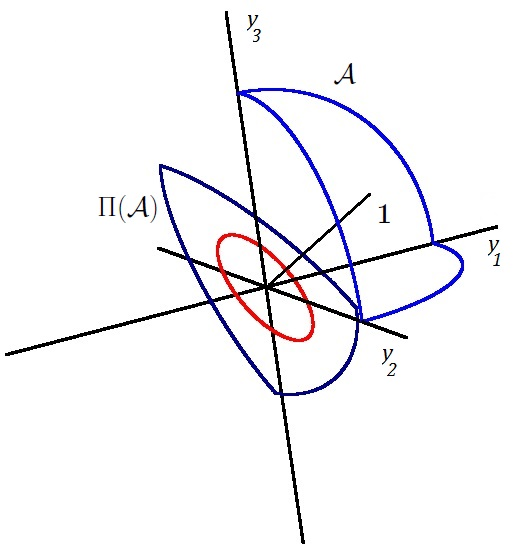
\includegraphics[width=2.75in]{minSS3dSampleSpace.jpg}
\caption{A depiction of $\mathcal{A}$, $\Pi(\mathcal{A})$, and the
  unit circle for the illustrative example where $b_{1}(\mathbf{1},\by)=\min(\by)=0$ and
  $s(\mathbf{1},\by)=\sum (y_i -b_{1}(\mathbf{1},\by))^2 =1$.
$\mathcal{A}$ is the combination of three quarter circles, one
  on each plane defined by $y_i=0$. The projection of this manifold
  onto the deviation space is depicted by the bowed triangular shape
  in the plane defined by $\sum y_i=0$. The circle in this plane
  represents the sample space for the intermediate sample $\bz^*$. Also
  depicted is the vector $\mathbf{1}$, the design matrix for the
  location and scale setting.}
\label{fig:sampSpace}
\end{figure}

%
\subsubsection{Evaluation of the proposal density} 
%Calculation of the appropriate Jacobian of the transformation is absolutely vital and also non-trivial. Writing the transformation from the unit sphere in deviation space to $\mathcal{A}$ in 
%two steps facilitates calculation of the Jacobian in two steps as written above. % \textcolor{blue}{added the following sentence, hopefully it helps}
We now explain each step in computing the Jacobian described above.
%the scale transformation from the unit sphere to $\Pi(\mathcal{A})$, {keeping in mind that the Jacobian of a transformation is simply the ratio of infinitesimal volumes along the tangents of the domain and range of the transformation. 
\vskip 0.05 in
\noindent
{\bf Scale from $\mathbb{S}$ to $\Pi(\mathcal{A})$} \\
The first step is constrained to $\mc{C}^\perp(X)$  and scales the initial $\bz^{*}$ to $\bz=\frac{s(X,\boldsymbol{y}_{obs})}{s(X, \boldsymbol{z}^{*})}\bz^{*}$. For the Jacobian, we consider two substeps: first, the distribution on  $\mathbb{S}$ is transformed to that along a sphere of radius $r=\|\bz\|={s(X,\boldsymbol{y}_{obs})}/{s(X, \boldsymbol{z}^{*})}$. By comparison of the volumes of these spheres, this transformation contributes a factor of $r^{-(n-p-1)}$ to the Jacobian. For the second substep, the sphere of radius $r$ is deformed onto $\Pi(\mathcal{A})$.  This deformation contributes an attenuation to the Jacobian equal to the ratio of infinitesimal volumes in the tangent spaces of the sphere and $\Pi(\mathcal{A})$ at $\bz$.  
Restricting to $\mc{C}^\perp(X)$, this ratio is the cosine of the angle between the normal 
vectors of the two sets at $\bz$.  The normal to the sphere is its radius vector $\bz$. The normal to
$\Pi(\mathcal{A})$ is given in the following lemma with proof provided in the Appendix.  Gradients denoted by $\nabla$ are with respect to the data vector.
\begin{lemma}
\label{gradSTheoremReg}
Assume that conditions \ref{fullRank}-\ref{supReal}, \ref{as}, and \ref{regIn} hold and $\by\in \mathcal{A}$. Let 
$\nabla s(X,\by)$ denote the
gradient of the scale statistic with respect to the data vector evaluated at
$\by$.  Then $\nabla s(X,\by)\in \mc{C}^\perp(X)$ and is 
normal to $\Pi(\mathcal{A})$ at $\bz=Q\by$  in $\mc{C}^\perp(X)$.
\end{lemma}
As a result of the lemma, the contribution to the Jacobian of this attenuation is 
\begin{equation}
\label{cosine}
\cos(\gamma)=\frac{\nabla s(X,\by)^\top \bz}{\|\nabla
s(X,\by)\| \|\bz\|},
\end{equation}
where $\gamma$ is the angle between the two normal vectors.
This step is visualized in Figure~\ref{fig:stretchDeform} for the notional
location-scale example.  The figure pictures only $\mathcal{C}^{\perp}(X)$,
which in this case is a plane. The unit sphere (here, the
solid circle) is stretched to the dashed sphere, contributing
$r^{-(n-p-1)}$ to the Jacobian as seen in panel (a). In panel (b), the
dashed circle is transformed onto $\Pi(\mc A)$, contributing
$\cos(\gamma)$ to the Jacobian. The normal vectors in panel (b) are
orthogonal to the tangent vectors of $\Pi(\mc A)$ and the circle. 

\begin{figure}[t]
\centering
{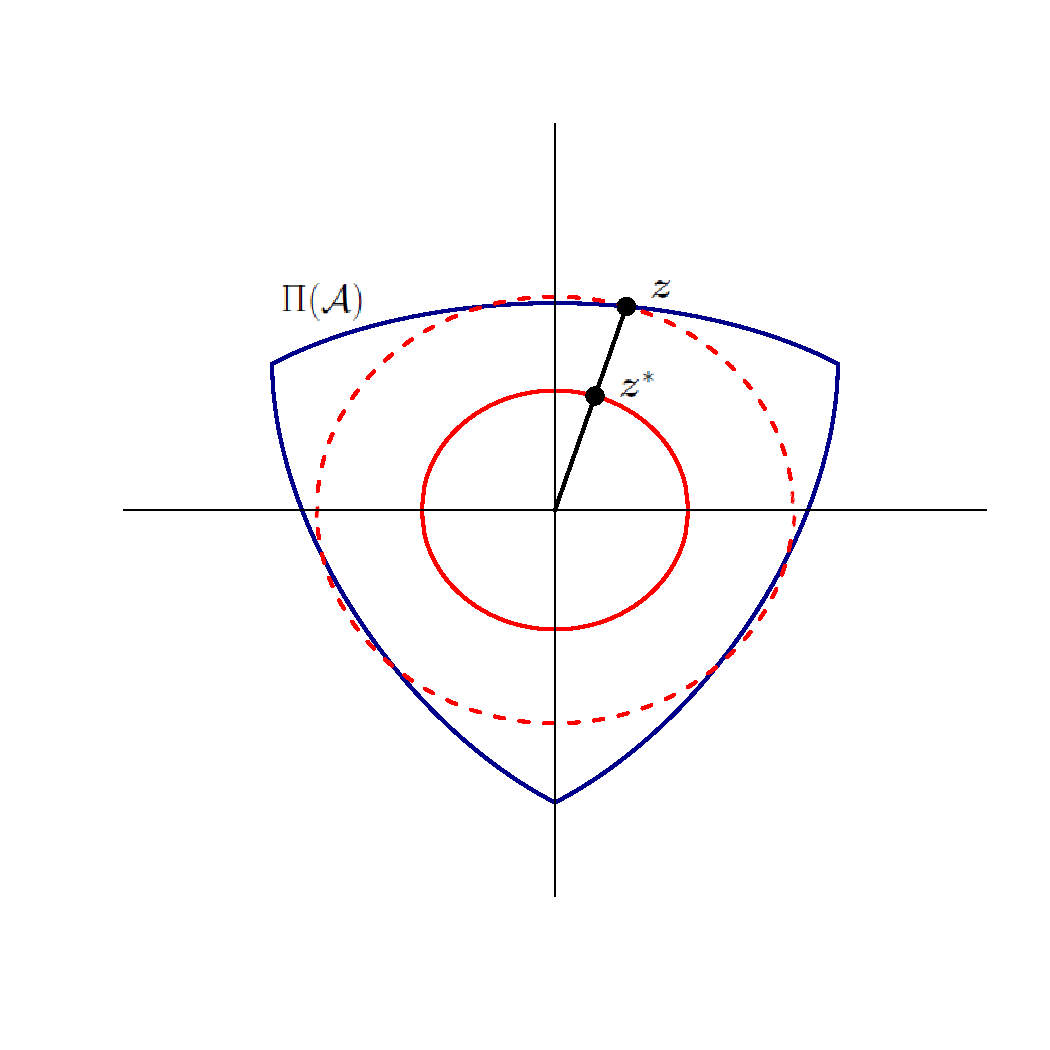
\includegraphics[width=2.9in]{minSSZSpace3.pdf}}
{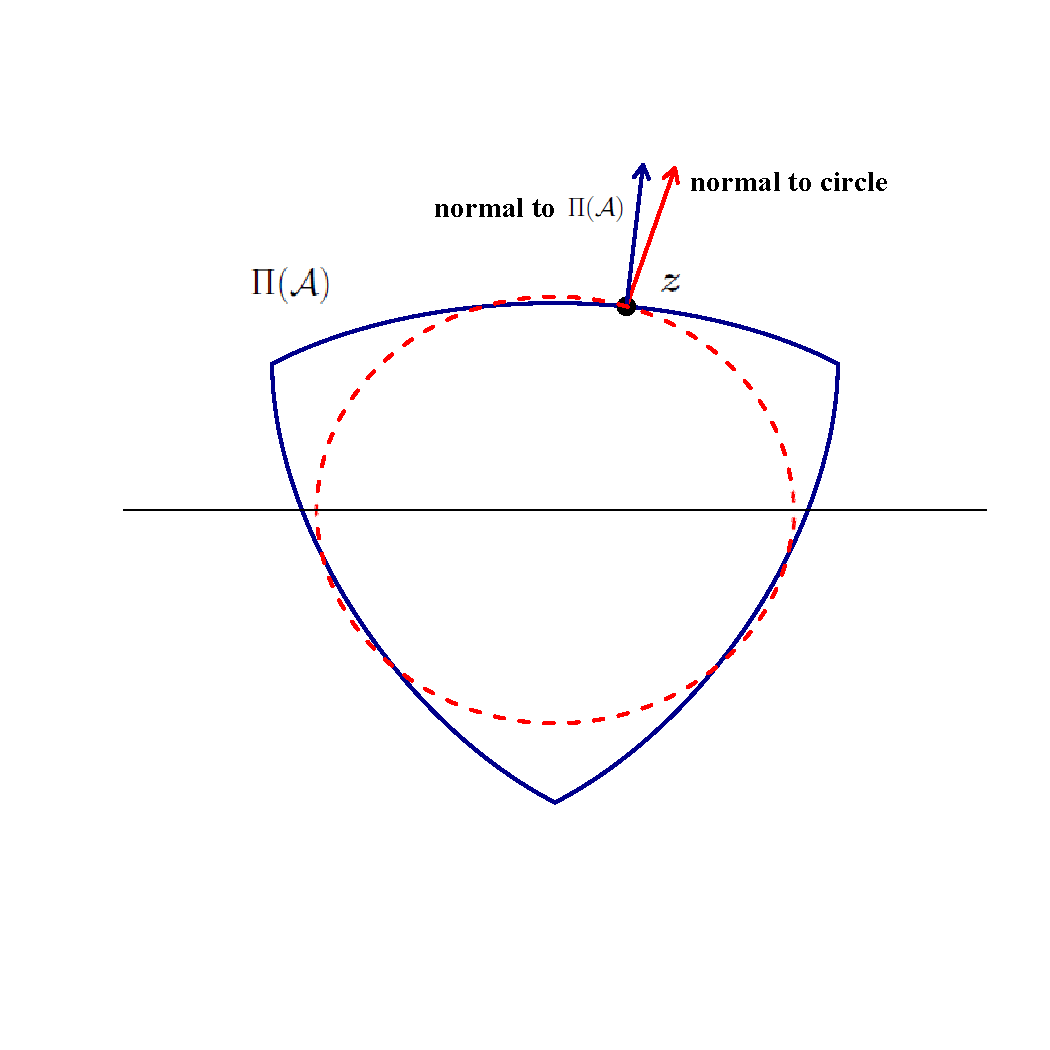
\includegraphics[width=2.9in]{minSSZSpace5.pdf}}
\caption{Visualization of the scaling from $z^{*}$ to $z$. Left: the first substep scales $z^{*}$ on the unit circle to the circle of radius $r = ||z||$, resulting in a change-of-variables transformation for the unit circle to a circle of radius $r$. The contribution to the Jacobian of this transformation is $r^{-(n-p-1)}$. Right: The second substep accounts for the the change-of-variables transformation from the circle of radius $r$ to $\Pi(\mathcal{A})$. The normal vectors to these two sets are used to calculate the contribution to the Jacobian of this part of the transformation are shown in the figure.}
\label{fig:stretchDeform}
\end{figure}



\vskip 0.05 in
\noindent
{\bf Shift from $\Pi(\mathcal{A})$ to $\mathcal{A}$} \\
The final piece of the Jacobian comes from the transformation from
$\Pi(\mathcal{A})$ to $\mathcal{A}$.  %For this we return to the full $n$ dimensional space.  
This step involves a shift of
$\bz$ to $\by$ along the column space of $X$. Since the shift depends on 
$\bz$, the density on the set 
$\Pi(\mathcal{A})$ is deformed by the shift. The
contribution of this deformation to the Jacobian is, again,
the ratio of the infinitesimal volumes along $\Pi(\mathcal{A})$ at $\bz$ to the
corresponding volume along $\mathcal{A}$ at $\by$. 
The ratio is calculated by considering the volume of the
projection of a unit hypercube in the tangent space of $\mathcal{A}$
at $\by$ onto $\mc{C}^\perp(X)$.
Computational details are
given in the following lemmas and subsequent theorem. Proofs of the lemmas are given in the appendix and the theorem is a direct result of the lemmas. Throughout, let
$\mc T_{y}(\mc A)$ and $\mc T_{y}^{\perp}(\mc A)$ denote the tangent
space to $\mc A$ at $\by$ and its orthogonal complement, respectively. %All gradients denoted by $\nabla$ are with respect to the data vector.
\begin{lemma}
\label{lem:basis}
Assume that conditions \ref{fullRank}-\ref{regEq} and \ref{regIn}-\ref{scaleEq2Reg} hold.  Then the $p+1$ gradient vectors 
$\nabla s(X,\by), \nabla b_1(X,\by),\dots, \nabla b_p(X,\by)$ form a
basis for $\mc T_{y}^\perp(\mc A)$ with probability one.
\end{lemma}

The lemma describes construction of a basis for $\mc T_{y}^\perp(\mc A)$, leading to a 
basis for $\mc T_{y}(\mc A)$.  Both of these bases can be orthonormalized.  
Let $A=[a_{1},\dots,a_{n-p-1}]$  and $B=[b_1,\dots,b_{p+1}]$ denote the 
matrices whose columns contain the orthonormal bases for  $\mc T_{y}(\mc A)$ and  $\mc T^{\perp}_{y}(\mc A)$, respectively.  
The columns in $A$ define a unit hypercube in $\mc T_{y}(\mc
  A)$ and their projections onto $\mc{C}^\perp(X)$ define a parallelepiped.
We defer construction of $A$ until later. 

\begin{lemma}
\label{lem:fullrank}
Assume that conditions \ref{fullRank}-\ref{regEq} and \ref{regIn}-\ref{scaleEq2Reg} hold.  
Then the $n\times (n-p-1)$ dimensional matrix $P=QA$ is of full column rank.
\end{lemma}

As a consequence of this lemma, 
the parallelepiped spanned by the columns of $P$ is not
degenerate (it is $n-p-1$ dimensional), and its volume
is given by
\begin{equation}
\label{eq:volume}
\text{Vol} (P) := \sqrt{\text{det}(P^\top P)}=\prod_{i=1}^{r} \sigma_i
\end{equation}
where $r=\text{rank} (P)=n-p-1$ and $\sigma_1\geq
\sigma_2\geq\dots\geq\sigma_r>0$ are the singular values of $P$ (e.g.,
\cite{miao1992}). 
Combining Lemmas \ref{lem:basis} and \ref{lem:fullrank} above leaves us with the following result concerning the calculation of the desired Jacobian.  
\begin{theorem}
\label{Jacobian}
Assume that conditions \ref{fullRank}-\ref{regEq} and \ref{regIn}-\ref{scaleEq2Reg} hold.  Then the
Jacobian of the transformation from the distribution along 
$\Pi(\mc A)$ to that along $\mc A $ is equal to the volume given in \eqref{eq:volume}.
\end{theorem}

\vskip 0.05 in
\noindent
{\bf The proposal density} \\
Putting all the pieces of the Jacobian together we have the following result. Any dependence on other variables, including current states in the Markov chain, is made implicit. 
\begin{theorem} 
Assume that conditions \ref{fullRank}-\ref{scaleEq2Reg} hold.  Let $\bz^{*}$ be sampled on the unit sphere in $\mc {C}^\perp (X)$ with density $p(\bz^{*})$.  Using the transformation of $\bz^*$ to $\by\in \mc A$ described in Theorem \ref{Transformation}, the density of $\by$ is
\begin{equation}
\label{dens:ystst}
p(\by)=p(\bz^*) r^{-(n-p-1)} \cos(\gamma)\text{Vol} (P)
\end{equation}
where $r={s(X,\boldsymbol{y}_{obs})}/{s(X,  \boldsymbol{z}^{*})}$,
and $\cos(\gamma)$ and $\text{Vol} (P)$ are as in equations \eqref{cosine} and \eqref{eq:volume}, respectively. 
\end{theorem} 
%\response{The proposal is governed by the choice of $p(z^{*})$ and a poor choice could cause concern about the efficiency of the convergence of the MCMC algorithm. For all the examples in the paper we defined $p(z^{*})$ to simply be the uniform distribution on $\mathbb{S}$. The advantage of this choice is that it requires no further tuning parameters and we have noticed good mixing in terms of the ability of the chain to generate new data $\mb y$ that is accepted with reasonable probabilities. To implement in practice, we simply generate an n-dimensional independent standard normal $\mb y^{*}$ for the proposal and transform this via $h(\cdot)$. Theoretically, the random normal vector would be projected onto $\mc{C}^{\perp}(X)$ and scaled to unit norm to generate the uniform on $\mathbb{S}$. Using simple algebra and conditions \ref{regEq}-\ref{scaleEq2Reg}, one can show $h(\cdot)$ is invariant to this projection and scaling. Another option for the proposal suggested by a reviewer that the authors have yet to study is generating a random walk. As we are proposing values on a complex manifold, it might be possible to implement this by conducting the random walk on $\mb y^{*}$ before transforming via $h(\cdot)$. This could provide some advantages in some situations, though we have yet to run into any serious issues with convergence using the independent proposal we utilize here.}
\response{The proposal is governed by the choice of $p(z^{*})$ and a poor choice could lead to an inefficient MCMC algorithm. For all examples in this paper we defined $p(z^{*})$ to be the uniform distribution on $\mathbb{S}$. The advantage of this choice is that it requires no further tuning parameters.  We have noticed good mixing in terms of the ability of the chain to generate new data $\mb y$ that is accepted with a reasonable probability. To implement the method in practice, we generate an n-dimensional independent standard normal $\mb y^{*}$ for the proposal and transform this via $h(\cdot)$. Theoretically, the random normal vector would be projected onto $\mc{C}^{\perp}(X)$ and scaled to unit norm to generate the uniform on $\mathbb{S}$. Using simple algebra and conditions \ref{regEq}-\ref{scaleEq2Reg}, one can show that $h(\cdot)$ is invariant to this projection and scaling. Another option for the proposal suggested by a reviewer that the authors have yet to study is generating a random walk. As we are proposing values on a complicated manifold, it might be possible to implement this by conducting the random walk on $\mb y^{*}$ before transforming via $h(\cdot)$. This could provide advantages in some situations, though we have yet to run into any serious issues with convergence using the independence proposal we utilize here.}

%In practice, computing $A$ directly to find $P$ and $\text{Vol} (P)$ is computationally intensive as it involves orthogonalization of $n$ vectors in $n$-dimensional space. 
Some details for computing the needed quantities are worth further explanation. Computing $\text{Vol} (P)$ involves finding an orthornormal matrix $A$ whose columns span $\mc T_{y}(\mc A)$. This matrix can be found by supplementing $B$ with a set of $n$ linearly independent columns on the right, and applying Gram-Schmidt orthonormalization.  The computational complexity of this step is $\mc O(n^3)$.  This is infeasibly slow when $n$ is large because it must be repeated at each iterate of the MCMC when a complete data set is drawn.  However, using results related to \textit{principal angles} found in \cite{miao1992} the volume \eqref{eq:volume} can be computed using only $B$. $B$ is constructed by Gram-Schmidt orthogonalization of $\nabla s(X,\by), \nabla b_1(X,\by),\dots, \nabla b_p(X,\by)$, reducing the computational complexity to $\mc O(np^2)$--a 
considerable reduction in computational burden when $n \gg p$. 
%Further, the singular values of $P=QA$ are also the singular values of
%$W^\top A$ where $Q=WW^{\top}$, which can be easily obtained through $B$.
The following corollary formally states how computation of $A$ can be circumvented. 
\begin{corollary}
\label{theorem:sings}
Let $U$ be a matrix whose columns form an orthonormal basis for $\mc C (X)$ and set $Q=WW^{\top}$ where the columns of $W$ form an orthonormal basis for $\mc{C}^\perp(X)$. Then the non-unit singular values of $U^\top B$ are the same as the non-unit singular values of $W^\top A$.
\end{corollary} 
\noindent The lemma implies that $\text{Vol} (P)$ is the product of the singular values of $U^\top B$. 

Second, the gradients of $\nabla s(X,\by), \nabla b_1(X,\by),\dots, \nabla b_p(X,\by)$ are easily computed in many cases. For example, below we consider M-estimators defined by the estimating equations:
\begin{eqnarray}
\label{Mest}
 \sum_{i=1}^n \psi\left(\frac{y_i - x_{i}^{\top}\bb(\by,X)}{s(\by,X)}\right) x_{ij}=0, \
 \sum_{i=1}^n \chi\left(\frac{y_i - x_{i}^{\top}\bb(\by,X)}{s(\by,X)}\right)=0, 
 \end{eqnarray} 
for $j = 1, 2, \dots, p$, $x_{ij}$ are the components of $x_{j}$ and  $\psi$ and $\chi$ are almost surely differentiable. The gradients can be found by differentiating this system of equations with respect to each $y_{i}$. In theory, finite differences could also be used as an approximation if needed. 
%{\bf John - for the finite differences, is this to approximate the gradient? }

%\response{Finally, it is clear the estimators themselves must be computed for every iteration of the Markov Chain. We have found this burden to be marginal in relation with respect to computing the needed Jacobian. In the simulations and real data analyses presented below, we will see that the additional burden is often of added value over traditional robust regression when substantial prior information is available that is not swamped by current data.}
\response{Finally, it is clear the estimators themselves must be computed for every iteration of the Markov Chain. We have found this burden to be marginal relative to computation of the needed Jacobian. In the simulations and real data analyses presented below, we will see that the additional computational expense needed to fit the Bayesian model is often worthwhile, leading to better performance compared to traditional, non-Bayesian robust regression estimators.  This is most evident when substantive prior information is available and information in the data is limited.}

%%%%%%%%%%%%%%%%%%%%%%%%%%%%%%%%%%%%%%%%%%%%%%%%%%%%%%%%%%%%
%
% Applications
%
%%%%%%%%%%%%%%%%%%%%%%%%%%%%%%%%%%%%%%%%%%%%%%%%%%%%%%%%%%%%
%\section{Applications}
%In this section we apply the restricted likelihood to both simulated and real data. 

\section{Simulated Data}
\label{simData}
We study the performance of restricted likelihood methods in two simulation settings. The first is a hierarchical setting. The second is a variable selection setting where there are several potential covariates where only a few have non-zero effect sizes.

\subsection{Simulation 1}
The first is a hierarchical setting where the data are contaminated with outliers. Specifically, simulated data come from the following model:\begin{align}
\label{gensim2}
\begin{split}
& \theta_{i}  \sim   N(\mu, \tau^{2}),  \ i = 1, 2, \dots, 90  \\ 
& y_{ij} \sim (1-p_{i})N(\theta_{i}, \sigma^{2}) + p_{i}N(\theta_{i}, m_{i}\sigma^{2}),\  j = 1, 2,..., n_{i}
\end{split}
\end{align}
with $\mu = 0, \tau^{2} = 1, \sigma^{2} = 4$. The values of $p_{i}, m_{i}$, and $n_{i}$ depend on the group and are formed using 5 replicates of the full factorial design over factors $p_{i},m_{i},n_{i}$ with levels $p_{i} = .1, .2, .3$, $m_{i} = 9, 25$, and $n_{i} = 25, 50, 100$. This results in 90 groups that have varying levels of outlier contamination and sample size. We wish to build models that offer good prediction for the good portion of data within each group. The full model for fitting is a corresponding normal model without contamination:
\begin{equation}
\label{fullsim2}
\begin{split}
%& \mu \propto 1, \  \tau^{2} \propto \tau^{-2}, \\
& \theta_{i}\sim N(\mu, \tau^{2}), \  \sigma^{2}_{i} \sim IG(a_{s}, b_{s}),  \ i = 1, 2, \dots, 90, \\ 
& y_{ij}\sim  N(\theta_{i},\sigma^{2}_{i}), \ j = 1, 2, \dots, n_{i}.
\end{split}
\end{equation}
For the restricted likelihood versions we condition on robust M-estimators of location and scale in each group: $T_{i}(y_{i1}, \dots, y_{in_{i}}) = (\hat\theta_{i}, \hat\sigma^{2}_{i}), i = 1, 2, ..., 90$.  These estimators are solutions to equation \eqref{Mest} (where $x_{i}\equiv 1$) with user specified $\psi$ and $\chi$ functions designed to discount outliers. The two versions use Huber's and Tukey's $\psi$ function, while both versions use Huber's $\chi$ function. The tuning parameters associated with these functions are chosen so that the estimators are $95\%$ efficient under normally distributed data. These classical M-estimators are commonly used in robust regression settings  \citep{huber2009}.  %We will see that his choice has some interesting effects on the results. %These estimators are implemented in the R function \texttt{MASS::rlm} with \cite{huber2009} providing further details. 

To complete the specification of model \eqref{fullsim2}, the hyperparameters $\mu, \tau^{2}, a_{s}$, and $b_{s}$ must be given priors or fixed. The joint prior density for $\mu$ and $\tau^{2}$ is improper and proportional to $\tau^{-2}$. The pair $a_{s}$ and $b_{s}$ are fixed to a variety of values representing different levels of prior knowledge. For each pair, we set $b_{s} = 4a_{s}c$ resulting in a prior mean for each $\sigma^{2}_{i}$ of $\frac{4ca_{s}}{a_{s}-1}, \ a_{s} >1$. The precision is $\frac{(a_{s} -1)^{2}(a_{s}-2)}{(4ca_{s})^{2}}$, meaning larger $a_{s}$ and smaller $c$ result in a more informative prior. With $c = 1$ the shrinkage (for large $a_{s}$) is to the true value of $\sigma^{2} = 4$. We consider $a_{s} = 1.25,  5, 10$ and $c = 0.5, 1, 2$ for a total of nine different priors. 


$K = 30$ data sets are generated from \eqref{gensim2}. For each data set and each pair $(a_{s}, c)$, the Bayesian models are fit using MCMC. The MCMC for the restricted likelihood version requires no computational details other than those described for the traditional Bayesian model in Section \ref{BayesLinMod}. This is because there are conditioning statistics for each group and the model's conditional independence between the groups allows the data augmentation described earlier to be performed independently within each group. That is, there is a separate Gibbs step for each group to generate the group level data matching the statistics for that group. \response{The acceptance rates for newly generated data across all groups and simulations ranged from $0.57$ to $0.68$}

\response{To asses the predictive capability, we seek a metric that takes into account both the estimation of $\theta_{i}$ and $\sigma^{2}$. In this model, estimation of $\theta_{i}$ and prediction are analogous. To this end we consider the loss:
\begin{equation}
\label{sim1loss}
L((\hat\theta_{i}, \hat\sigma_{i}), (\theta_{i},\sigma)) =
\log(\hat\sigma_{i}^{2}) - \log(\sigma^{2}) + \frac{1}{\hat\sigma_{i}^{2}}(\sigma^{2} + (\theta_{i} - \hat{\theta_{i}})^{2})
\end{equation}
Note, this loss is proportional to the Kullback-Leibler divergence between two normals with the base normal being the true distribution of the good portion of the data and the the other normal representing the estimate under the fitting method. We are using fixed point estimates $\hat\theta_{i}$ and $\hat\sigma$ which are posterior means under the Bayesian models and the standard point estimates for the classical methods.
}
%To assess predictive capability, the models are compared using Kullback-Leibler (KL) divergence from the distribution of good data to the posterior predictive distribution. Specifically, for the $i^{th}$ group of the $k^{th}$ simulated data set $\by_{k}$ compute:
%\begin{equation}
%\label{kl}
%KL^{(M)}_{ik} = \int \log \frac{f(\tilde y | \theta_{i}, \sigma^{2})}{f_{i}(\tilde y | M, \by_{k})}  f(\tilde y | \theta_{i}, \sigma^{2}) \ dy
%\end{equation}
%where $M$ indexes the fitting model and $f(\tilde y | \theta_{i}, \sigma^{2}) = N(\tilde y | \theta_{i}, \sigma^{2})$, the normal density function with (known) mean $\theta_{i}$ and variance $\sigma^{2}$, evaluated at $\tilde y$. For the Bayesian models, ${f_{i}(\tilde y | M, \by_{k})} = \int f(\tilde y |\theta_{i}, \sigma_{i}^{2}) \pi(\theta_{i}, \sigma^{2}_{i} | M, \by_{k})d\theta_{i}d\sigma^{2}_{i}$ where $\pi(\theta_{i}, \sigma^{2}_{i} | M, \by_{k})$ is the posterior for the $i^{th}$ group model parameters under model $M$ for the $k^{th}$ data set. $M$ denotes either the full normal theory model \eqref{fullsim2} or one of the two restricted likelihood versions, along with specified $a_{s}$ and $c$. For the classical robust fits, we set $f_{i}(\tilde y | M, \by_{k}) = N(\tilde y|\hat\theta_{i}, \hat\sigma^{2}_{i})$ as a groupwise plug-in estimator for the predictive distribution. The classical fits are computed separately for each group with no consideration of the hierarchical structure between the groups. The overall mean $\overline{KL}^{(M)}_{{\cdot}{\cdot}} = \frac{1}{90K} \sum_{k = 1}^{K} \sum_{i=1}^{90} KL^{(M)}_{ik}$ is used to compare the models, where smaller means correspond to better fits. Sampling variation is summarized with the standard error between the $K=30$ replicates in the simulation:  $SE(\overline{KL}^{(M)}_{{\cdot} k}) = \sqrt{\frac{1}{K(K-1)}\sum_{k = 1}^{K} (\overline{KL}^{(M)}_{{\cdot} k} - \overline{KL}^{(M)}_{{\cdot}{\cdot}})^{2}}$ where $\overline{KL}^{(M)}_{{\cdot} k} = \frac{1}{90}\sum_{i = 1}^{90} KL^{(M)}_{ik}$.
Figure \ref{kl_sim} displays the average of loss \ref{sim1loss} grouped by pairs of $a_{s}$ and $c$ with error bars plus/minus on standard error within the group.  The values of $a_{s}$ and $c$, do not affect the classical robust linear models. The average loss for the normal theory models ranges from $1.44$ to $1.66$ and are left out of the figure. For $c = 0.5$ and $c = 1$ the results favor the restricted likelihood methods as seen by the lower values of loss. The choice of $c = 2$ corresponds to a particularly poor prior distribution.  The prior has substantial mass above $\sigma^{2} = 4$, with prior means for $\sigma^2$ from $8.9$ to $32$ as $a_s$ varies.  Additionally, the tuning parameters chosen for the location and scale estimators result in an upward bias in the estimate of $\sigma^{2}$. This bias depends on $m$ and $p$. For example, for $m = 9$ and $p = .1$, Huber's version converges to roughly $4.8$ as $n$ grows.  The bias is greater for more severe levels of contamination.  The alignment of biases in prior distribution and in likelihood from the summary statistic (when applied to the contaminated data) inflates the estimate of scale.  Not surprisingly, a poor prior distribution whose weakness matches the weakness in the likelihood results in poorer inference.  In this case, poorer than the classical estimators. 
 
\begin{figure}[t]
\centering
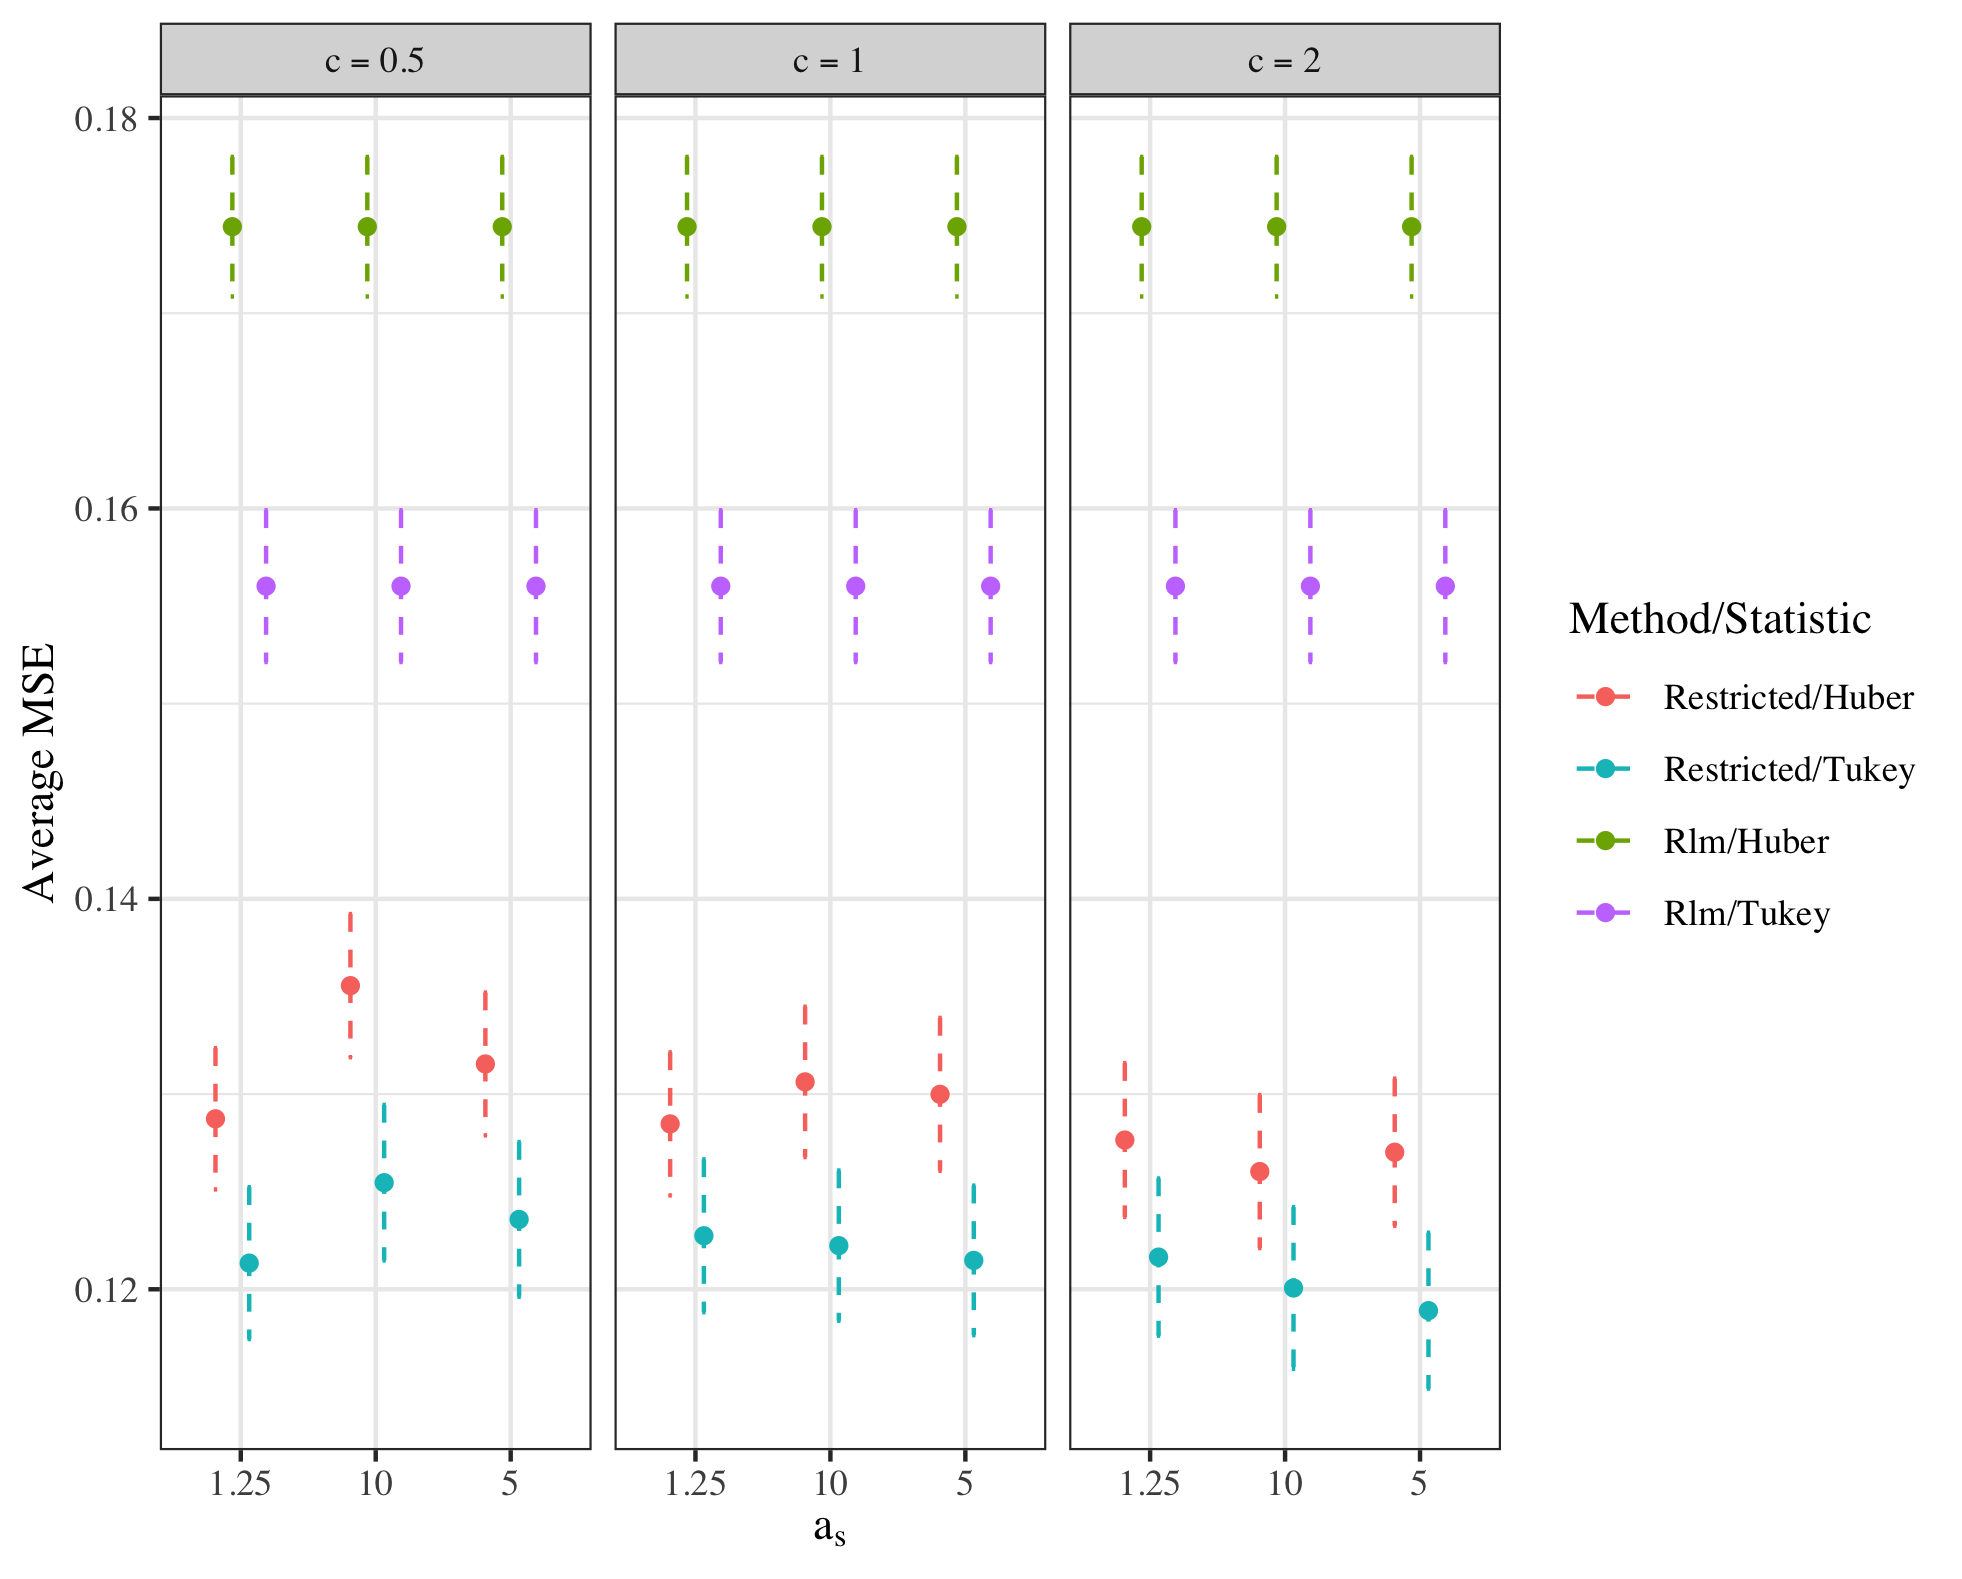
\includegraphics[width = 5in]{mse_sim2_facet_scale.png}
\caption{Average Loss plus/minus one standard error for each value of $a_{s}$ and $c$. Smaller values represent better fits. The panels correspond to $c = 0.5$ (left), $c=1$ (middle), and $c=2$ (right), with the values of $a_{s}$ on the horizontal axis. The average loss for the normal theory model ranges from $1.44$ to $1.66$ and is left out of the figure.}
\label{kl_sim}
\end{figure}

It is also interesting to consider the effects of factors $n$, $p$, and $m$.  We present the results for a single prior ($a_s = 5$ and $c = 1$).  For each simulation $k$, the main effect average loss is found for each factor $n$, $p$, and $m$. Figure \ref{kl_mnp} displays the average of these main effects over the $K = 30$ simulations along  with error bars plus/minus one standard error. For each group $n$, $p$, and $m$, the Bayesian restricted likelihood versions have better average loss than do the classical methods. As expected, the average loss gets larger as the contamination gets more severe (larger $m$ or larger $p$) and tends to get smaller as the sample size $n$ grows.  The advantage of the Bayesian method is greater for smaller sample sizes.  

\begin{figure}[t]
\centering
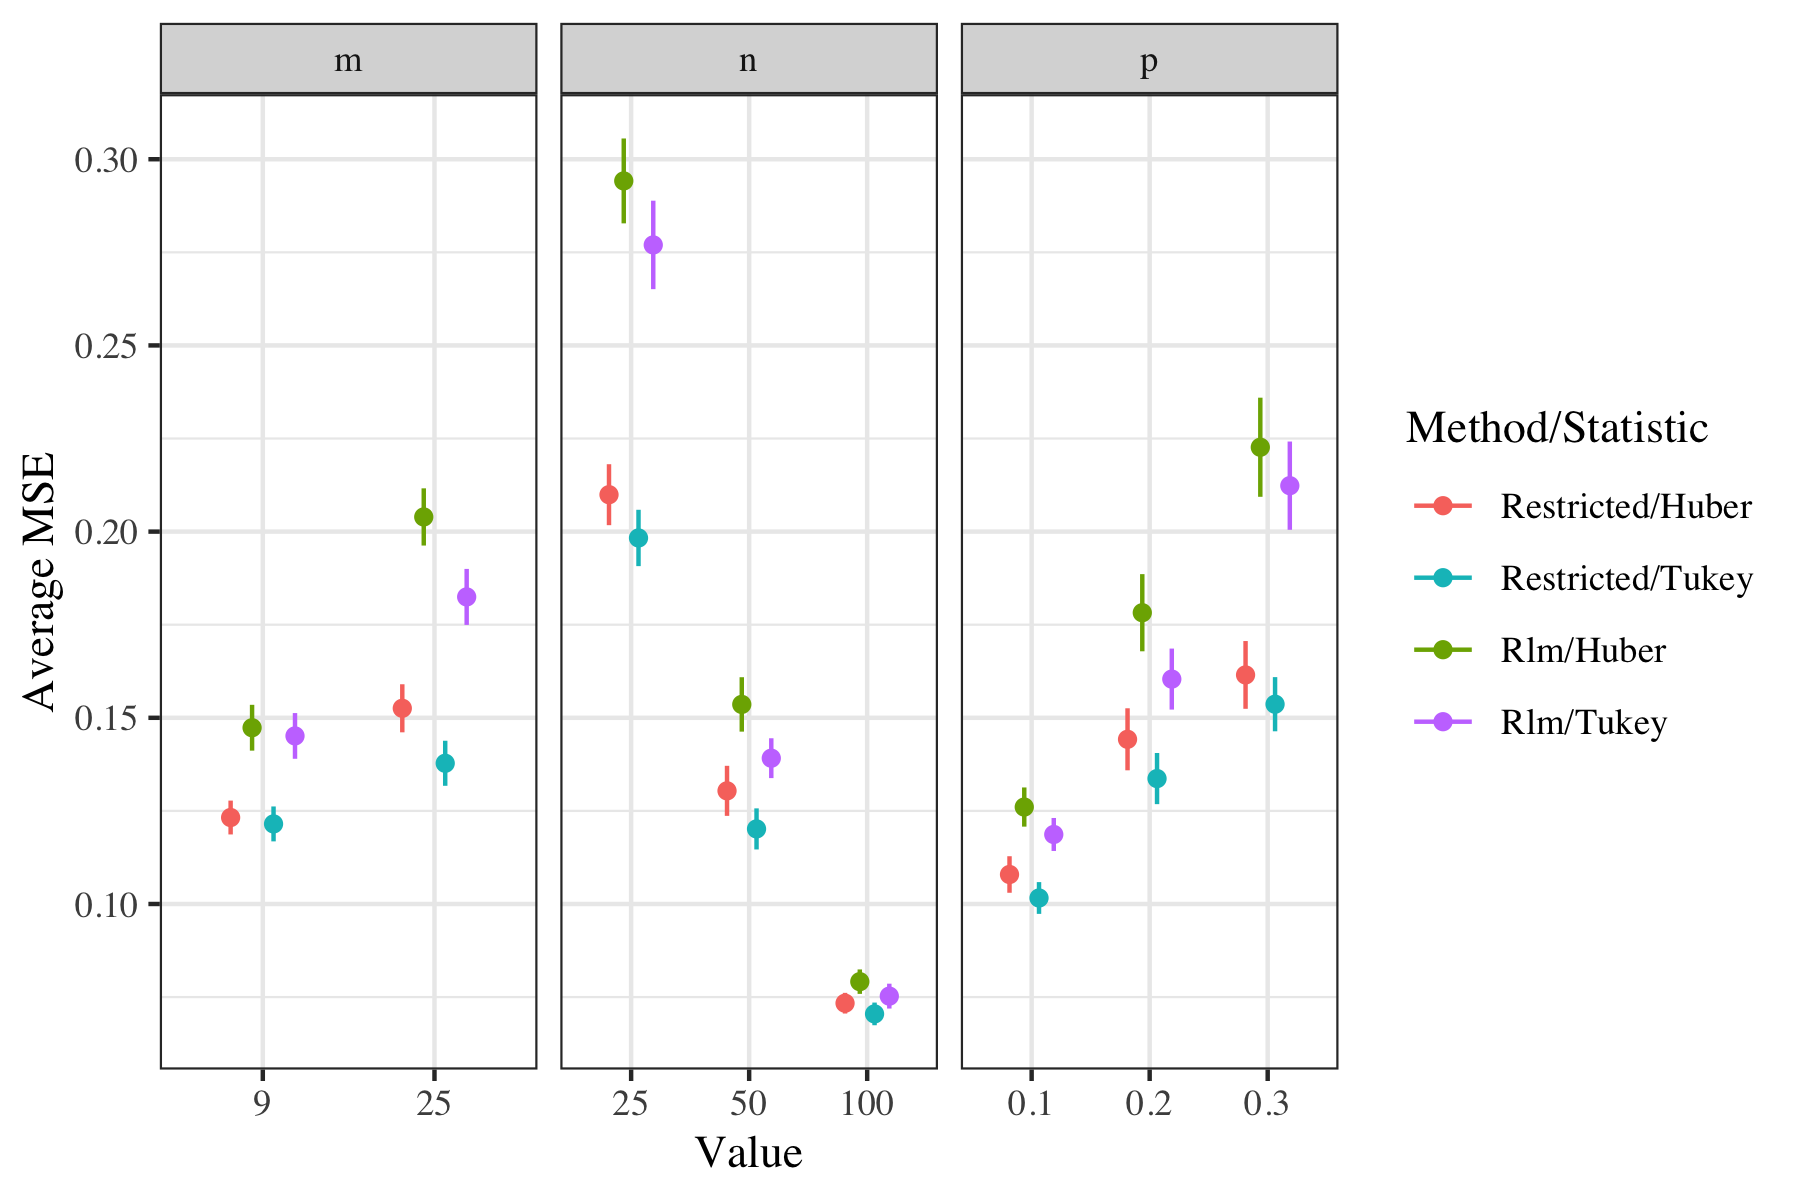
\includegraphics[width = 5in]{MSE_sim2_mnp.png}
\caption{Average loss plus/minus one standard error grouped by the factors $m$ (left), $n$ (middle), and $p$ (right). These results are for the single prior with $a_s = 5$ and $c = 1$.}
\label{kl_mnp}
\end{figure}

This simulation shows the potential of the restricted likelihood and conveys some cautions.  Specifically, the choice of summary statistics, along with corresponding tuning parameters is important. For the tuning parameters, we applied the default choice of $95\%$ efficiency at the normal.  Under the simulation model here, this choice results in bias in the scale estimation which affects the performance of the method. These choices must be made when using both the classical and Bayesian methods. The Bayesian approach encourages use of a hierarchical model structure and allows one to incorporate prior information in the analysis.  These features can improve predictive performance substantially.  If poorly handled, they can, of course, harm performance.  


\subsection{\response{Simulation 2}}

In this simulation the data are generated from the following mechanism: $y = \bbeta^{\top}x + \epsilon$
with $\bbeta = (\beta_{1}, \beta_{2},\beta_{3})^{\top}$ and the error $\epsilon \sim N(0,\sigma^{2})$ with probability $0.8$ and $\epsilon \sim \text{Half-Normal}(0,25\sigma^{2})$ with probability $0.2$ (i.e., there is a relatively large amount of one-sided outlier contamination). The components of $x = (x_{1}, x_{2}, x_{3})$ are correlated with $x_1 \sim N(0,1)$ and $x_{j} = x_{1} + \eta_{j}$ with $\eta_{j} \sim N(0, 4)$ for $j = 2,3$. This results in a theoretical correlation of $1/sqrt(5) \approx 0.44$ between $x_{1}$ and both $x_{j}, j = 2, 3$. The model used for fitting contains an additional 27 covariates, some of which are also correlated with $x_{1}$, $x_{2}$, and $x_{3}$. Specifically the fitting model is $y = \beta^{\top} x + \beta^{*\top} x^{*} + \epsilon$ where $x^{*}$ and $\beta^{*}$ are 27 dimensional vectors of extra covariates and slope parameters. Of these 27 covariates, 21 are generated independently from standard normal distributions. Of the remaining 6, two each are generated by adding standard normal noise to $x_{1}$, $x_{2}$, and $x_{3}$. This represents a common situation where several covariates with various levels of correlation amongst them are available for fitting, but only a few govern the data generating mechanism.

For the simulation, $K = 30$ data sets (including the additional covariates) of size $n = 500$ are generated from the true model with true values $\bbeta = (1,1,1)^{\top}$ and $\sigma^{2} = 2$. We fit the model including all 30 covariates and consider the following methods for the fit 1) classical robust regression with Tukey's estimator of location and Huber's estimator of scale, 2) the corresponding restricted likelihood version 3) A heavy-tailed Bayesian model with a Student-t likelihood with $\nu = 5$ degrees of freedom.  For the Bayesian models we take $\bbeta_{all}\sim N_{20}(\mb{0}, \sigma^{2}_{\beta}I)$ with $\bbeta_{all} = (\bbeta, \bbeta^{*})^{\top}$ and $\sigma^{2}\sim IG(5,8)$ under the restricted model and  $\sigma^{2}\sim IG(5,\frac{\nu-2}{\nu}8)$ under the Student-t model.  For each data set, we fit the models for $ \sigma_{\beta} = 0.4, 0.6, 0.8,\dots, 1.4$. The acceptance rates for the restricted likelihood MCMC data-augmentation step range from $0.3$ to $0.36$ across all the data sets and values of $\sigma_{\beta}$. To compare performance we first consider the $MSE = (||\bbeta - \hat\bbeta||^{2} + ||\hat\bbeta^{*}||^{2})/30$ for each simulation where $\hat\bbeta$ and $\hat\bbeta^{*}$ are point estimates for the fitted model. For the Bayesian models, we use posterior means. The average MSE plus/minus one standard error over the simulations for each $\sigma^{2}_{\beta}$ are displayed in Figure \ref{mseSimMany}. The classical fit is labeled `rlm` and is the same for each value of the prior standard deviation $\sigma^{2}_{\beta}$. We see for most values of the the prior standard deviation, the Bayesian models (`restricted' and `t') outperform the classical fit. The correlation amongst the covariates causes a certain level of confounding and the prior shrinkage helps to improve estimation. However, too much shrinkage can be detrimental as demonstrated for $\sigma_{\beta} = 0.4$. While this will help for estimation of $\bbeta^{*} = 0$, the estimation of the active parameters $\bbeta$ can be hindered. The $t$ model seems more sensitive to this effect than the restricted model. The restricted model also has an additional advantage when it comes to prediction of the non-outlying data. To see this, for each simulation we consider the mean negative log-likelihood of the non-outlying data: $MNLL = -\frac{1}{N} \sum \log f(y_{i} |  \hat\bbeta, \hat\bbeta^{*}, \hat\sigma)$ where $f$ is the assumed likelihood and the average is taken over the $N$ non-outlying points $y_{i}$. For the classical and restricted fits, $f$ is the normal likelihood and for the `t' it is the heavy-tailed Student-t likelihood. The average MNLL plus/minus one standard error over the simulations for each $\sigma^{2}_{\beta}$ are displayed in Figure \ref{negllSimMany}. First, the restricted version has a small but consistent improvement over the classical method. Second, it is clear that that the heavy-tailed model suffers when trying to predict the non-outlying data since it assumes the entire data generating mechanism is heavy-tailed. 

\begin{figure}[t]
\centering
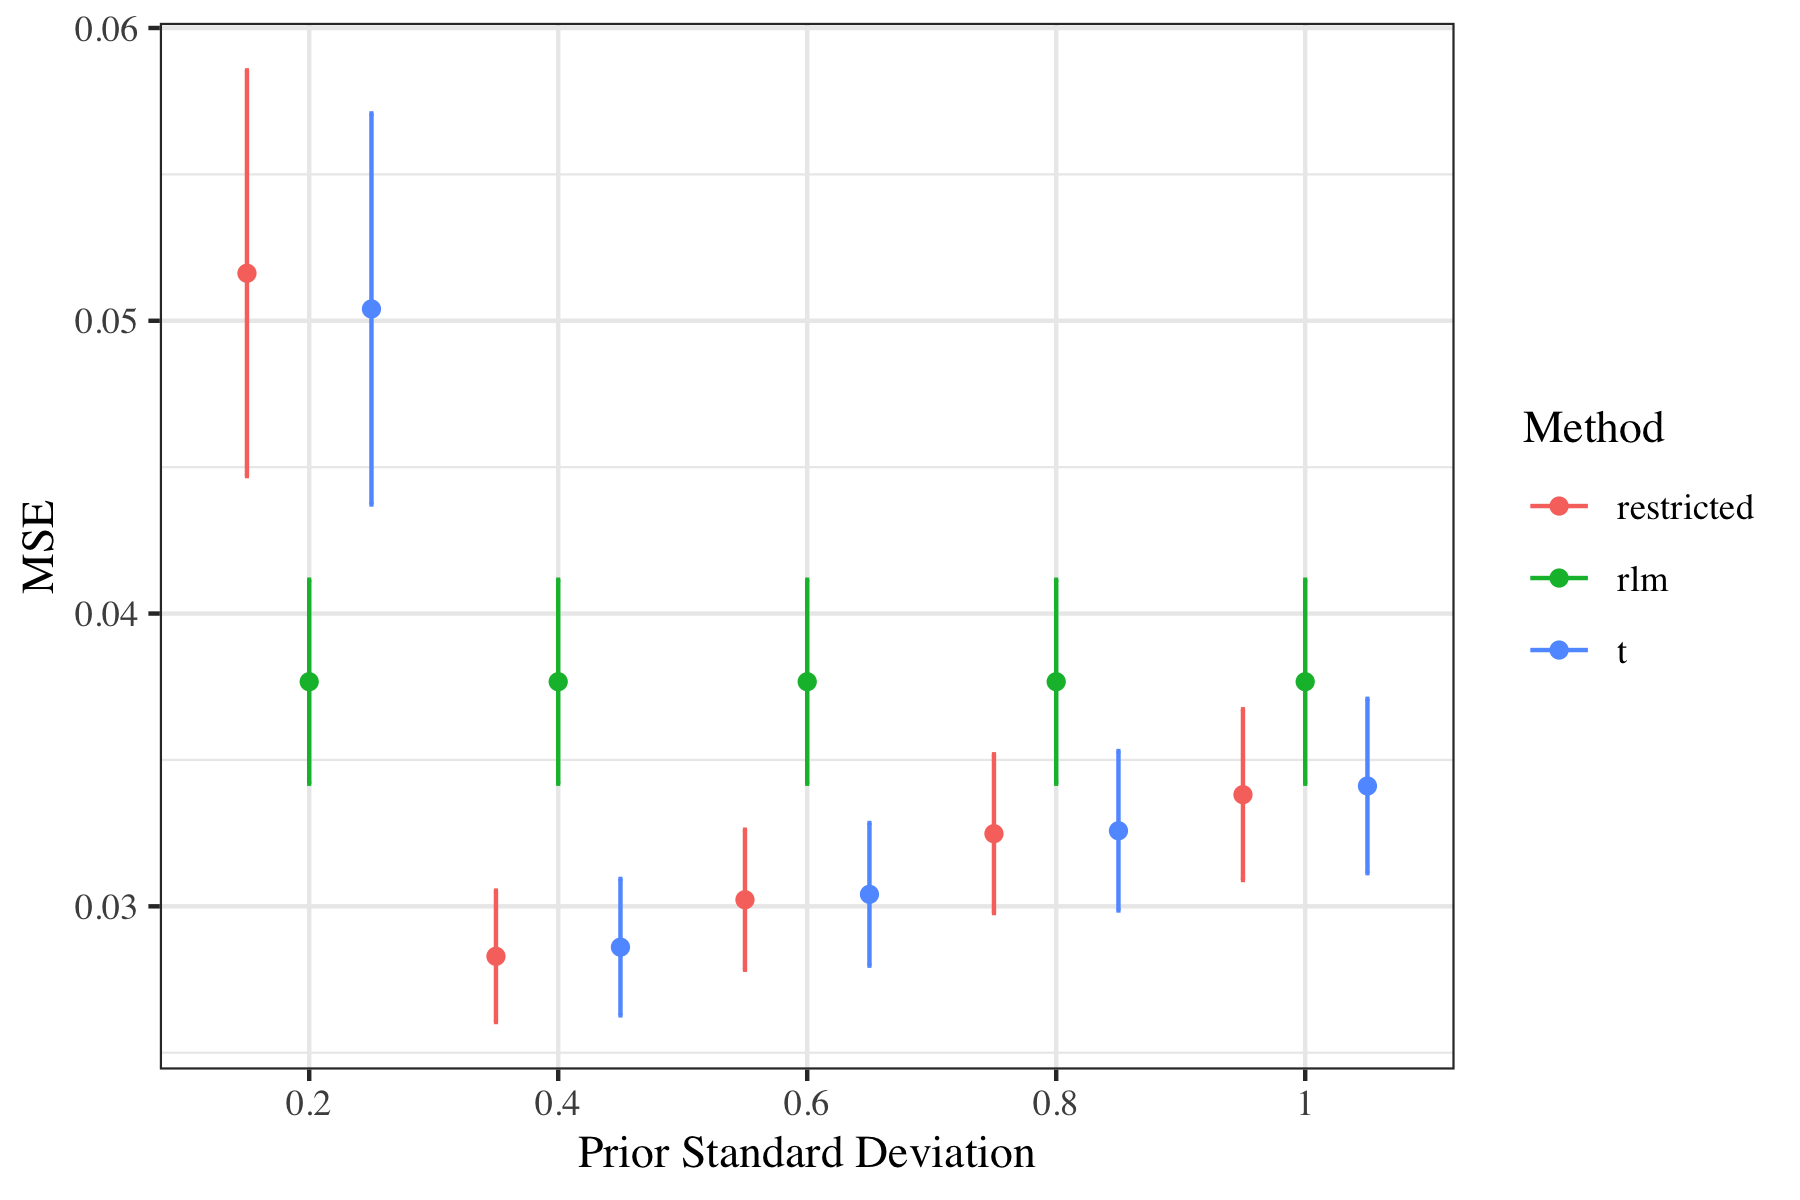
\includegraphics[width = 5in]{mse_sim_many_p.png}
\caption{Average MSE plus/minus one standard error over the $K = 30$ simulations for each value of the prior standard deviation ($\sigma^{2}_{\beta}$) and each of the fitting methods. `Restricted' is our method conditioning on Tukey's estimator of location and Huber's estimator of scale. `rlm' refers to the classical robust linear model fit with the same estimators and `t' is the heavy-tailed Bayesian model with a Student-t likelihood. The `rlm' results are the same for each $\sigma^{2}_{\beta}$.}
\label{mseSimMany}
\end{figure}

\begin{figure}[t]
\centering
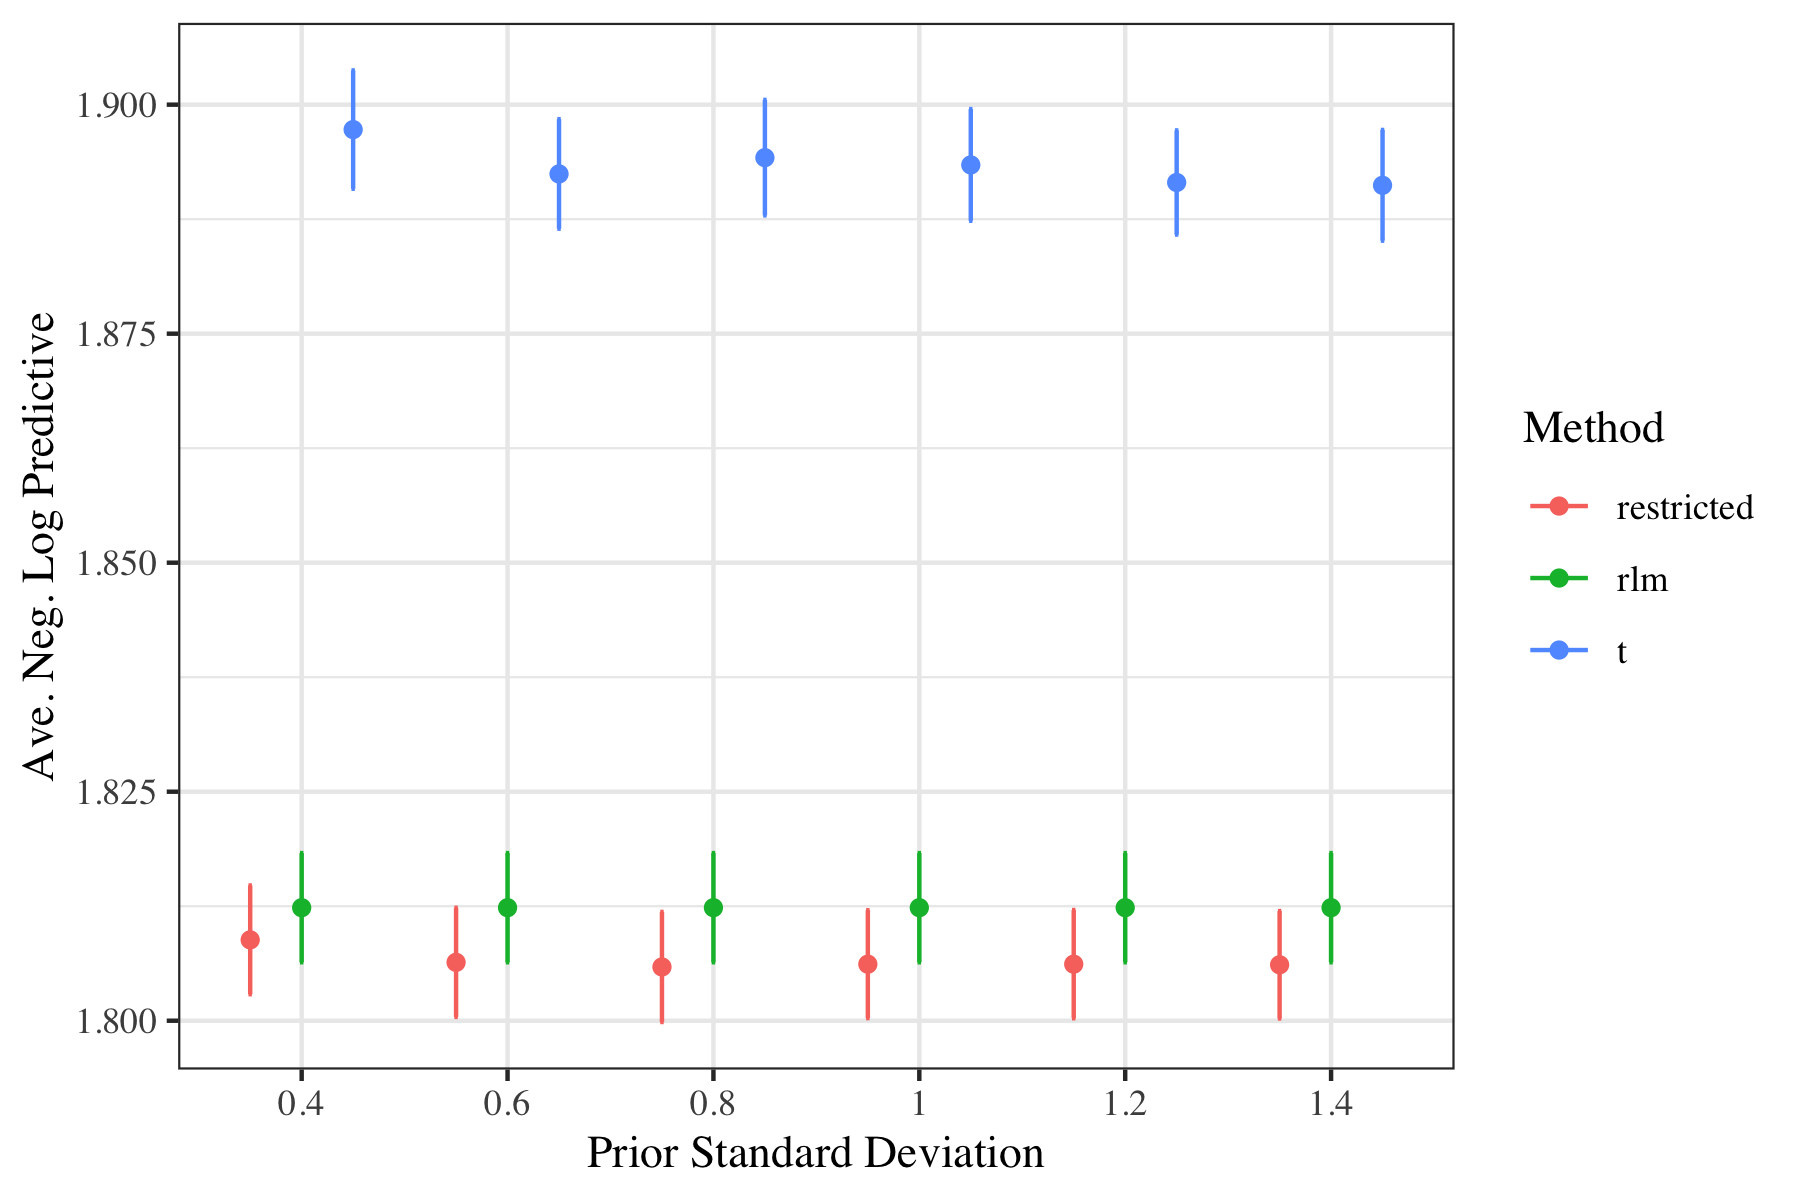
\includegraphics[width = 5in]{negll_sim_many_p.png}
\caption{Average MNLL plus/minus one standard error over the $K = 30$ simulations for each value of the prior standard deviation ($\sigma^{2}_{\beta}$) and each of the fitting methods. `Restricted' is our method conditioning on Tukey's estimator of location and Huber's estimator of scale. `rlm' refers to the classical robust linear model fit with the same estimators and `t' is the heavy-tailed Bayesian model with a Student-t likelihood. The `rlm' results are the same for each $\sigma^{2}_{\beta}$.}
\label{negllSimMany}
\end{figure}



%%%%%%%%%%%%%%%%%%%%%%%%%%%%%%%%%%%%%%%%%%%%%%%%%%%%%%%%%%%%
%
% Real data
%
%%%%%%%%%%%%%%%%%%%%%%%%%%%%%%%%%%%%%%%%%%%%%%%%%%%%%%%%%%%%
\section{Real Data}
\label{RealData}
We illustrate our methods with a pair of regression models for data from Nationwide Insurance Company that concern prediction of the performance of insurance agencies.

%%%%%%%%%%%%%%%%%%%%%%%%
%%NW data
%%%%%%%%%%%%%%%%%%%%%%%%
%
%\subsection{Nationwide Data}
Nationwide sells many of its insurance policies through agencies which provide direct service to policy holders.  The contractual agreements between Nationwide and these agencies vary.  Our interest is the prediction of future performance of agencies where  performance is measured by the total number of households an agency services (`household count'). 
 
The data are grouped by states with a varying number of agencies by state. Identifiers such as agency/agent names are removed. Likewise, state labels and agency types (identifying the varying contractual agreements) have been made generic to protect the proprietary nature of the data. Additionally, the counts were scaled to have standard deviation one before analysis. 

As an exploratory view, a plot of the square root of (scaled) household count in 2012, against that in 2010 
is shown in Figure \ref{fig:ctVct} for four states. The states have varying numbers of agencies and  the different colors represent the varying types of contractual agreements as they stood in 2010 (`Type').  A significant number of agencies closed sometime before 2012, as represented by the $0$ counts for 2012. Among the open agencies, linear correlations exists with strength depending on agency type and state.  `Type 1' agencies open in 2012 are of special interest.  One could easily subset the analysis to only these agencies, removing the others. However,  we leave them and use the data as a test bed for our techniques by fitting models that do not account for agency closures or contract type.  Our expectation is that the restricted likelihood will facilitate prediction for the `good' part of the data (i.e., open, `type 1' agencies).  \response{It is of concern to the company to predict closures and future performance for agencies that remain open. It is important for planning purposes that the predictions are not overly influenced by a handful of over/underperforming agencies. Our analysis focuses on one aspect of the business problem - the prediction of future performance for agencies, given they remain open.}  

\begin{figure}[t]
\centering
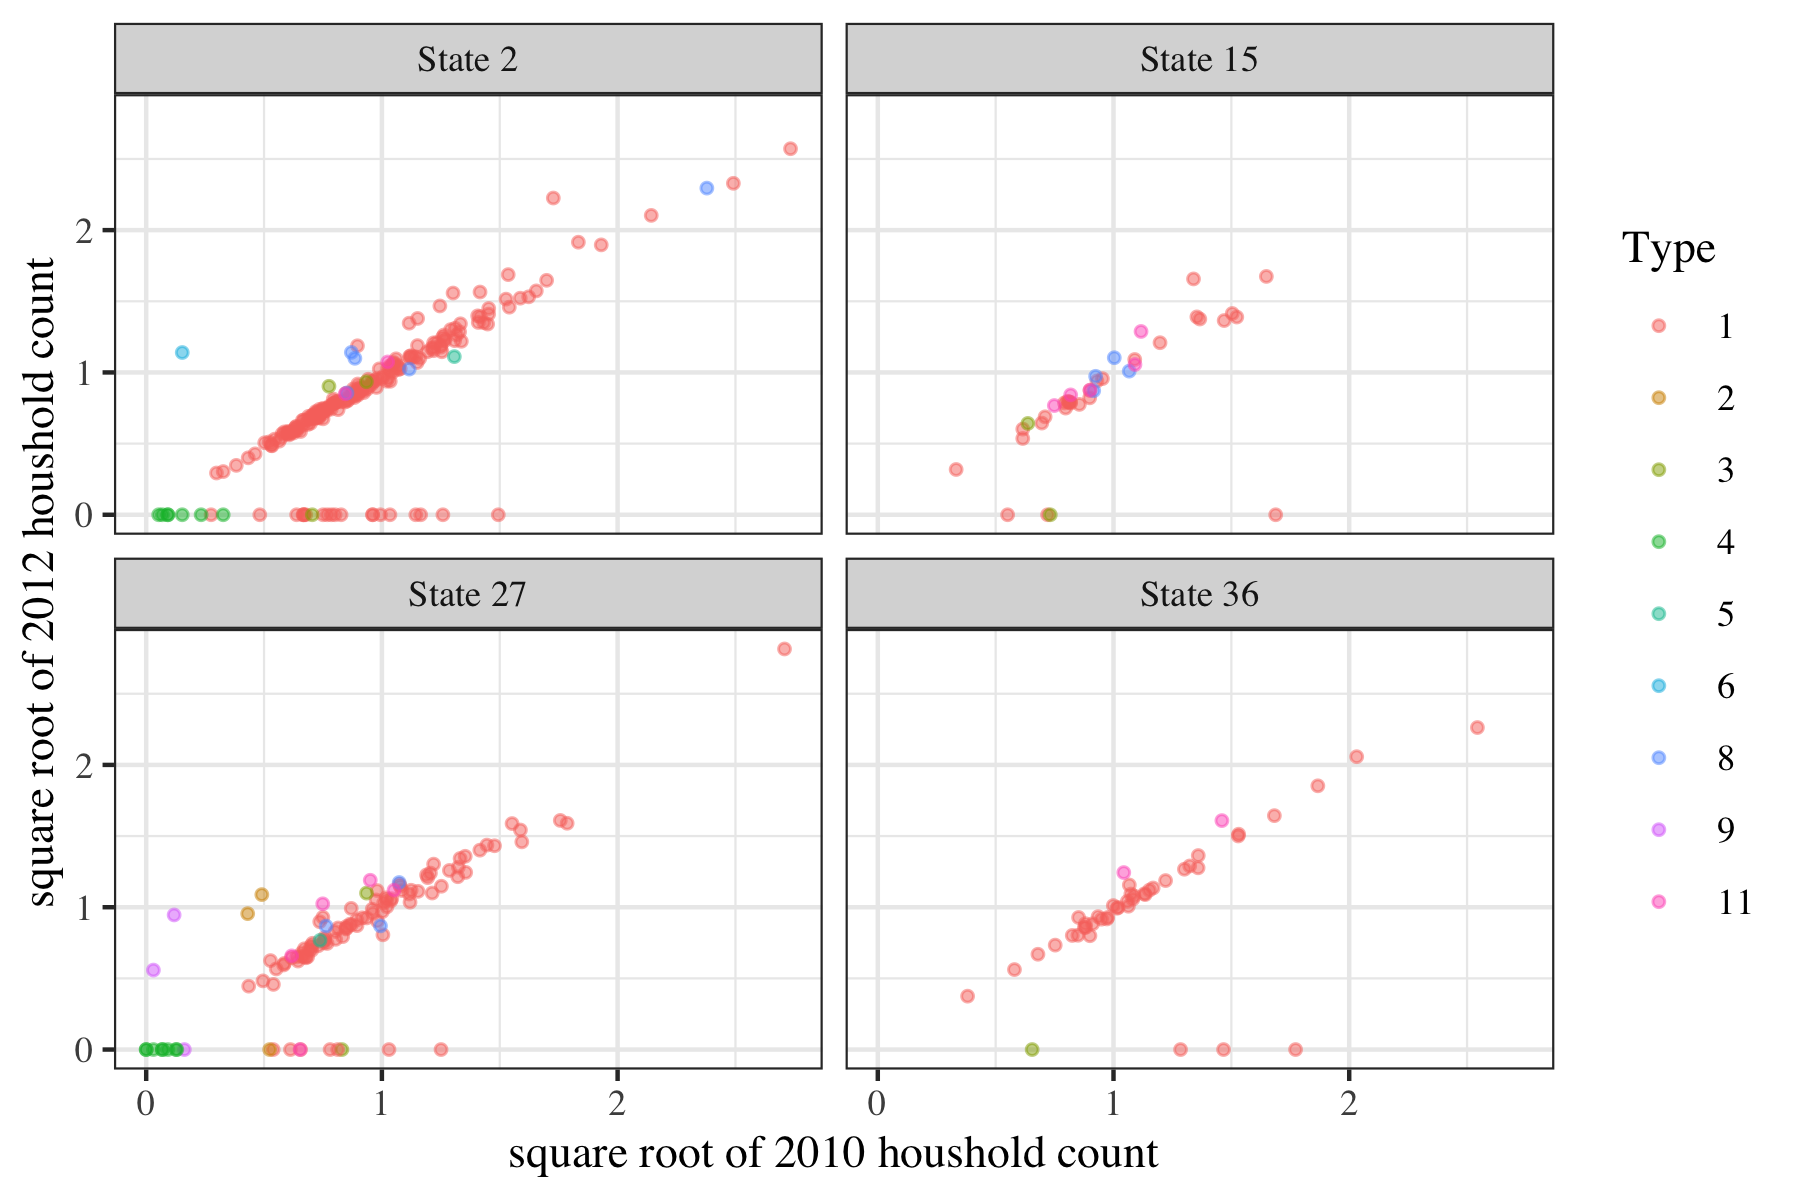
\includegraphics[width=5in]{scatter_by_state.png}
\caption{The square root of (scaled) count in 2012 versus that in 2010 for four states. The colors represent the varying contractual agreements as they stood in 2010 (`Type').  Agencies that closed during the 2010-2012 period are represented by the zero counts for 2012.}
\label{fig:ctVct}
\end{figure}

\subsection{State Level Regression model}
%\response{included two more covariates in the regression}

\label{regModelNW}
The first analysis is based on individual regressions fit separately within states.  The following normal theory regression model is used as the full model for a single state:
\begin{equation}
\label{eq:regModel}
\bbeta\sim N(\bmu_0, \Sigma_0);\ \ \sigma^2\sim IG(a_0,b_0);\ \  
y_{i}=\bx_{i}^{\top}\bbeta+\epsilon_{i},\ \ \epsilon_{i}\iid N(0, \sigma^2),\ i=1,\dots, n, 
\end{equation}
where $\bbeta$ is a three dimensional vector ($p=3$) of regression coefficients for the covariate vector $\bx_{i}$ consisting of the square root of household count in 2010, and two different size/experience measures related to the number of employees associated with the agency. The response, $y_{i}$ is the square root of household count in 2012.  
The hyper-parameters $a_0, b_0, \mu_0$ and $\sigma^{2}_0$ are all fixed and set from a 
robust regression fit to the corresponding state's data from the time period two years
before. Specifically, Let $\hat\bbeta$ and $\hat\sigma^{2}$ be estimates from the robust linear regression of 2010 counts on 2008 counts.  We fix $a_0 = 5$ and set $b_0 = \hat\sigma^{2}(a_0 - 1)$ so the prior mean is $\hat\sigma^{2}$. We set $\bmu_0 = \hat\bbeta$ and $\Sigma_0 =  n_{p}\hat\Sigma_{0}$ where $n_{p}$ is the number of agencies in the prior data set and $\hat\Sigma_{0}$ is the estimated covariance matrix of $\hat\bbeta$ derived from the robust regression. 
This prior is in the spirit of the Zellner's $g$-prior \citep{zellner1986, liang2008}.  In general, scaling the prior variance by a factor $g = n_{p}$ is analogous to the unit-information prior \citep{kass1995reference}, with the difference that we are using a prior data set, not the current data set, to set the prior. The obvious reason why this model is misspecified is due to omission of the contract type and agency closure information.  Closing our eyes to these variables, many of the cases appear as outliers. Additionally, the model assumes equal variance within each state, an assumption whose worth is arguable (see Figure \ref{fig:ctVct}). 

We compare four Bayesian models: the standard Bayesian normal theory model, two restricted likelihood models, both with simultaneous M-estimators, and a heavy-tailed model.  For the restricted likelihood methods we use the same simultaneous M-estimators as in the simulation of Section \ref{simData} adapted to linear regression.  The heavy-tailed model replaces the normal sampling density in \eqref{eq:regModel} with a $t$-distribution with $\nu = 5$ degrees of freedom. The Bayesian models are all fit using MCMC, with the restricted versions using the algorithm presented in Section \ref{highDim}. 
We also fit the corresponding classical robust regressions and a least squares regression.  

\subsubsection{Method of model comparison}
We wish to examine the performance of the models in a fashion that preserves the essential features of the 
problem.  Since we are concerned with outliers and model 
misspecification, we understand that our models are imperfect and prefer to use an out-of-sample measure of fit.  
This leads us to cross-validation.  We repeatedly split the data into training
and holdout data sets; fitting the model to the training data and assessing performance on the holdout data.  

The presence of numerous outliers in the data implies that both training and validation data will contain 
outliers.  For this reason, the evaluation must be robust to a certain fraction of bad data.  
The two main strategies are to robustify the evaluation function \citep[e.g.,][]{ronchetti1997} or 
to retain the desired evaluation function and trim cases \citep{jung2014}.  Here,
we pursue the trimming approach with log predictive density for the Bayesian models and log density from plug-in 
maximum likelihood for the classical fits used as the evaluation function.

The trimmed evaluation proceeds as follows in our context.  The evaluation function for case $i$ in the holdout data
is the log predictive density, say
$\log(f(y_i))$, with the conditioning on the 
summary statistic suppressed.  The trimming 
fraction is set at $0 \leq \alpha < 1$. To score a method,
we first identify a base method. Denote the predictive density under this method by $f_{b}(y)$.  Under the base method, $\log(f_{b}(y_i))$ is computed for each case in the 
holdout sample, say $i = 1, \ldots, M$.  Order the holdout sample according to the ordering of $\log(f_{b}(y_i))$ and denote this
ordering by $y_{(1)}^b, y_{(2)}^b, \dots, y_{(M)}^b$. That is, for $i<j$
$\log(f_{b}(y_{(i)}^b))<\log(f_{b}(y_{(j)}^b))$. All of the methods are then scored on the holdout sample with the mean trimmed log marginal pseudo likelihood, 
\[TLM_b(A) = (M - [\alpha M])^{-1} \sum_{i=[\alpha M]+1}^{M}
    \log(f_A(y_{(i)}^b)),\]
 where $f_A$ corresponds to the predictive
 distribution under the method ``A'' being scored.  In other words, the $[\alpha M]$ observations with the smallest values of $\log(f_{b}(y))$ are 
removed from the validation sample and all of the methods are scored using only the
remaining $M - [\alpha M]$ observations. Larger values of $TLM_b(A)$ indicate better predictive performance. This process is advantageous to the base method since the smallest scores from this method are guaranteed to be trimmed.  A method
that performs poorly when it is the base method is discredited.  %For a complete evaluation, we allow each method
%to appear as the base method.  For brevity, we present only a selection of results in our subsequent analyses.  

\subsubsection{Comparison of predictive performance}
%Model performance is assessed using the mean and standard deviation of the TLM 
%across $K = 50$ different splits into training and holdout samples. 
`Type 1' agencies are of special interest to the company and so the evaluation of the TLM is done on only holdout samples of `Type 1', whereas the training is done on agencies of all types. This is intended to demonstrate the robustness properties of the various methods. 
%First, we include all observations
%in each validation sample to calculate TLM for each split. We then
%repeat the evaluation using only certain subsets of the validation
%sample that are of special interest. Subsets include open agencies,
%open `Type 1' agencies, and `Type 1' agencies. For brevity, we include
%results for the `Type 1' agencies only. As noted, assessing model
%predictions on this set of agencies is of special interest to the
%company.  A range of training sample sizes was used and we include
%results from $n=25,100,1000,$ and $2000$ out of a total of $3180$ agencies. 
%The trimming fraction, $\alpha$, ranges from $0$ to $0.3$. A classical robust regression to the prior data assigns zero weight to around $16\%$ of observations; in essence removing these from the analysis. This informed the range of trimming fractions chosen.  
%In practice, we would set $\alpha$ slightly larger than $0.16$.  
Models are fit to four states labelled State 2, 15, 27, and 36, with $n = 222, 40, 117,$ and $46$, representing a range of sample sizes. Fitting is done on $K = 50$ training samples with training sample sizes taken to be $0.25n$ and $0.50n$. Holdout evaluation is done on the remaining (`Type 1') samples. The acceptance rates for  the data augmentation step,\response{for all but one training set}, range from  \response{$0.10$ to $0.8$} across the states, repetitions, and two versions of the model. \response{The exception was a single training set from State 15 resulting in an usually small acceptance rate under Tukey's version. This case didn't effect the overall results of the simulations but emphasizes the need to check convergence on a case by case basis.} The average $TLM_b(A)$ over the $K = 50$ training/holdout samples for the four states and seven methods are shown in Figure \ref{fig:tlm} where the base model is the Student-t model and $\alpha = 0.3$. Similar results are observed for other base models. The error bars are plus/minus one standard deviation of the average $TLM_b(A)$ over the $K = 50$  training/holdout samples. It is clear that the normal Bayesian model used as the full model (Normal) and the classical ordinary least squares fits (OLS) have poor performance due to the significant amount of outlier contamination in the data. In comparing our restricted methods to their corresponding classical methods, there is small, but consistent improvement across the states and training sample size. Additionally, variance reduction for the Bayesian versions is evident, especially in State 15, highlighted by the smaller error bars. For state 2, the largest state with $n = 222$, the restricted and classical robust methods have similar performance especially for larger training sample size. This reflects the diminishing effect of the prior as the sample size grows. Notably, the Student-t model performs poorly in comparison for this state. The predictive distribution explicitly accounts for heavy-tailed values, resulting in poorer predictions of the `good' data (i.e., the Type 1 agencies). Likewise, for State 27, another larger state, the Student-t model is outperformed by our restricted methods.   For the other states (State 15 and 36), the Student-t performs better to our restricted methods for smaller training sample size (25\% of the sample). However, this advantage goes away for the larger training sample size (50\% of the sample). Intuitively, as more data is available for fitting, more outliers appear and the heavy-tailed model compensates for them by assuming they come from the tails of the model; an assumption which is detrimental for prediction. Comparisons of the models depend on $\alpha$ as seen in Figure \ref{fig:tlmbyAlpha} which shows results for different $\alpha$ for training sample size $0.5n$. For smaller $\alpha$ (in this case $\alpha = 0.1$), many outliers are left untrimmed resulting in lower TLM  for all methods and noticeably larger standard deviation for the classical robust methods and our restricted likelihood. Larger values of $\alpha$ ensure that the predictive performance assessment excludes the majority of outliers. The proportion of $0$ counts in the data is roughly $0.14$, suggesting that $\alpha$ should be at least this large. 


%A mixture model could replace the heavy-tailed model. We assert it is more difficult to refine a mixture model in this setting reflecting the different types of outliers including the zero counts and agency types. The appeal of the restricted likelihood (and the classical robust approaches) is the avoidance of refining the model to capture (potentially transient) outlier generating mechanisms. Instead, the modeler focuses on estimating quantities of interest via statistics $T(\by)$. The improvement in our restricted likelihood versions over the classical robust fits is due to the informative prior distributions. In this case, similar data from previous years was used to formulate the prior. Like all Bayesian methods, performance is affected by the prior and it is important the prior accurately reflects the prior state of knowledge. 

\begin{figure}[t]
\centering
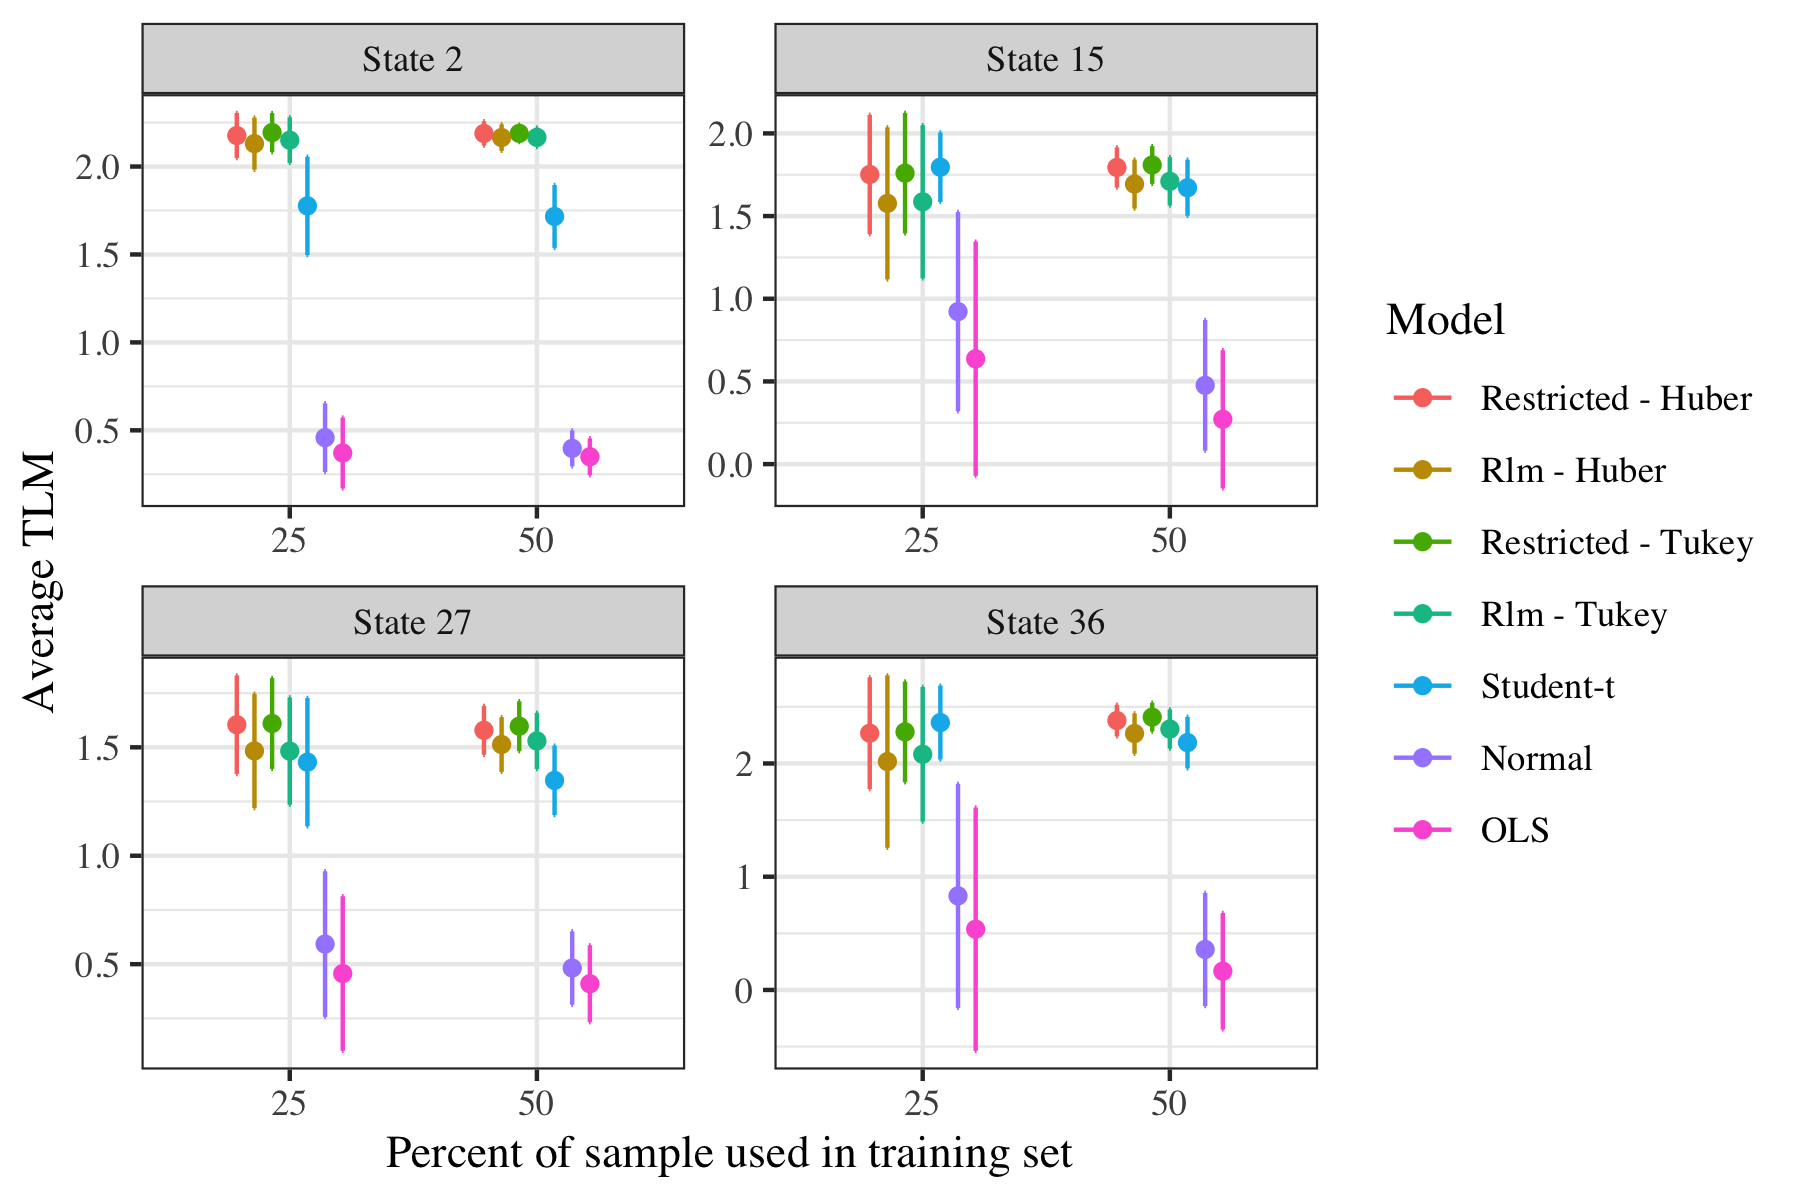
\includegraphics[width=6in]{tlm_base_Student-t.png}
\caption{Average TLM plus/minus one standard deviation over $K = 50$ splits into training and holdout samples. The panels are for the different states  2, 15, 27, and 36, with $n = 222, 40, 117,$ and $46$, respectively. The horizontal axis is the percent of $n$ used in each training set. The color corresponds to the fitting model.  Larger values of TLM are better.}
\label{fig:tlm}
\end{figure}

\begin{figure}[t]
\centering
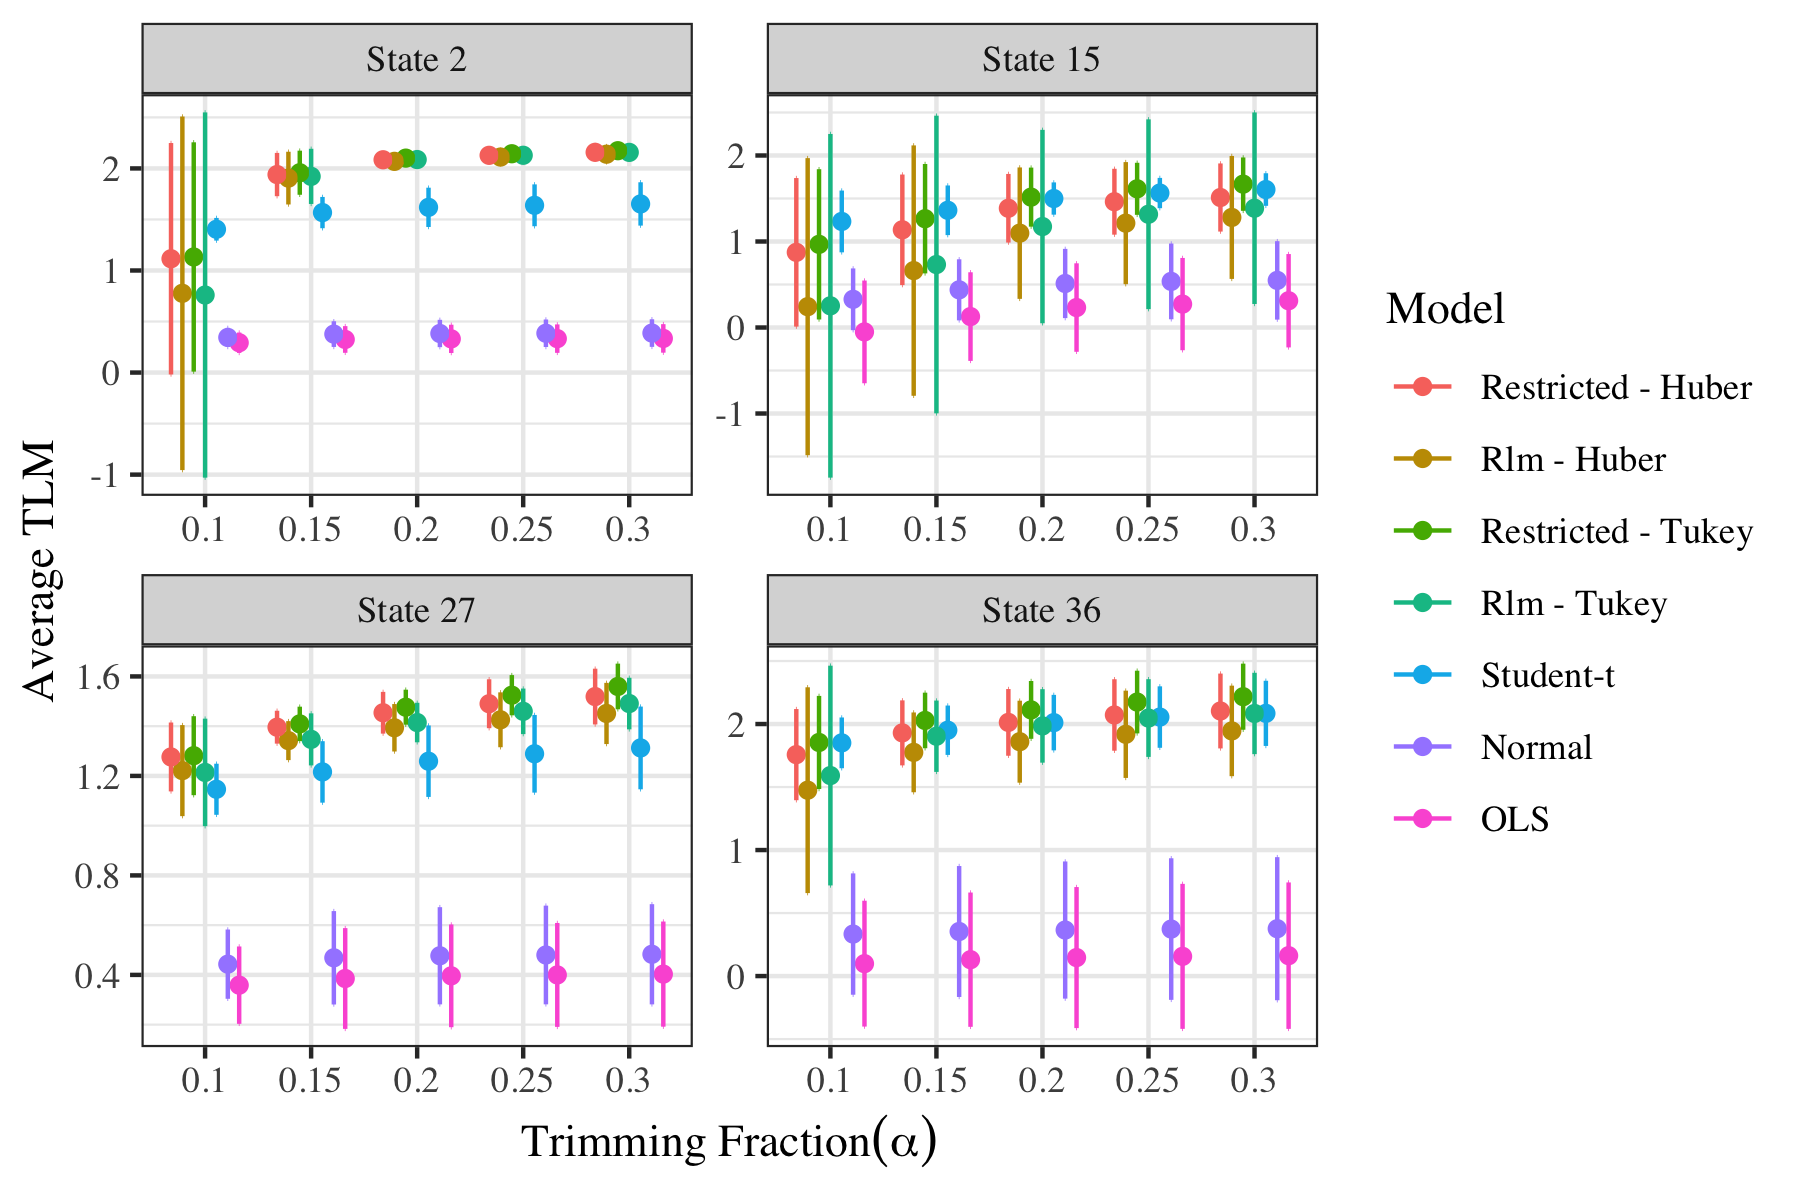
\includegraphics[width=6in]{tlm_base_Student-tbyTrimming.png}
\caption{Average TLM plus/minus one standard deviation over $K = 50$ splits into training and holdout samples for several values of the trimming fraction $\alpha$. The training sample size used is $0.5n$.  Larger values of TLM are better.}
\label{fig:tlmbyAlpha}
\end{figure}

%\begin{sidewaysfigure}
%\centering
%\captionsetup{justification=centering}
%%\subcaptionbox{}{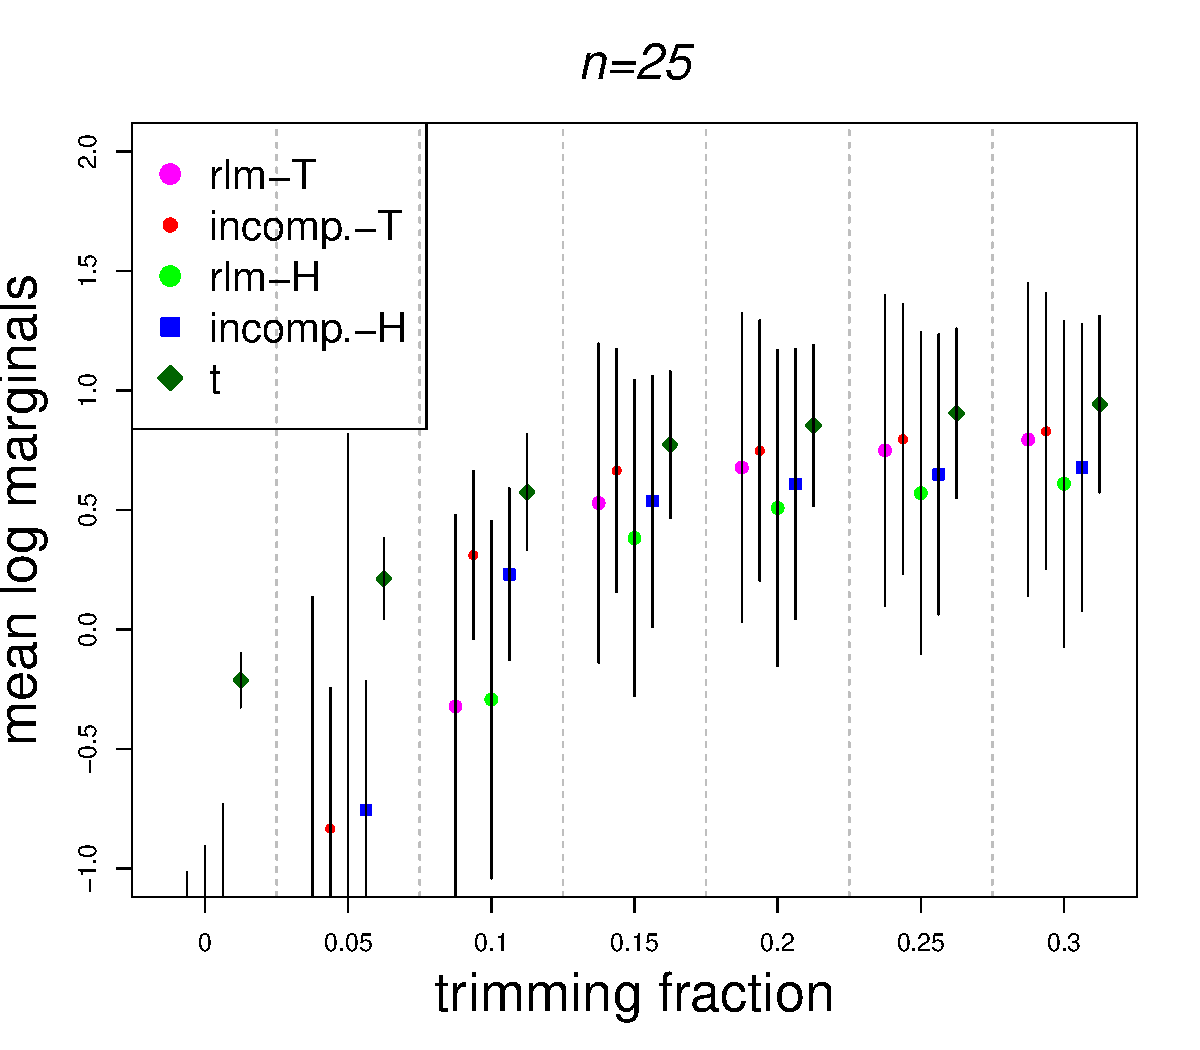
\includegraphics[width=\textwidth,page=1]{logMargType1AgenciesBaseModelt}}\quad
%%\subcaptionbox{}{\includegraphics[width=\textwidth,page=2]{logMargType1AgenciesBaseModelt}}\quad
%%\subcaptionbox{}{\includegraphics[width=\textwidth,page=3]{logMargType1AgenciesBaseModelt}}
%\subcaptionbox{}{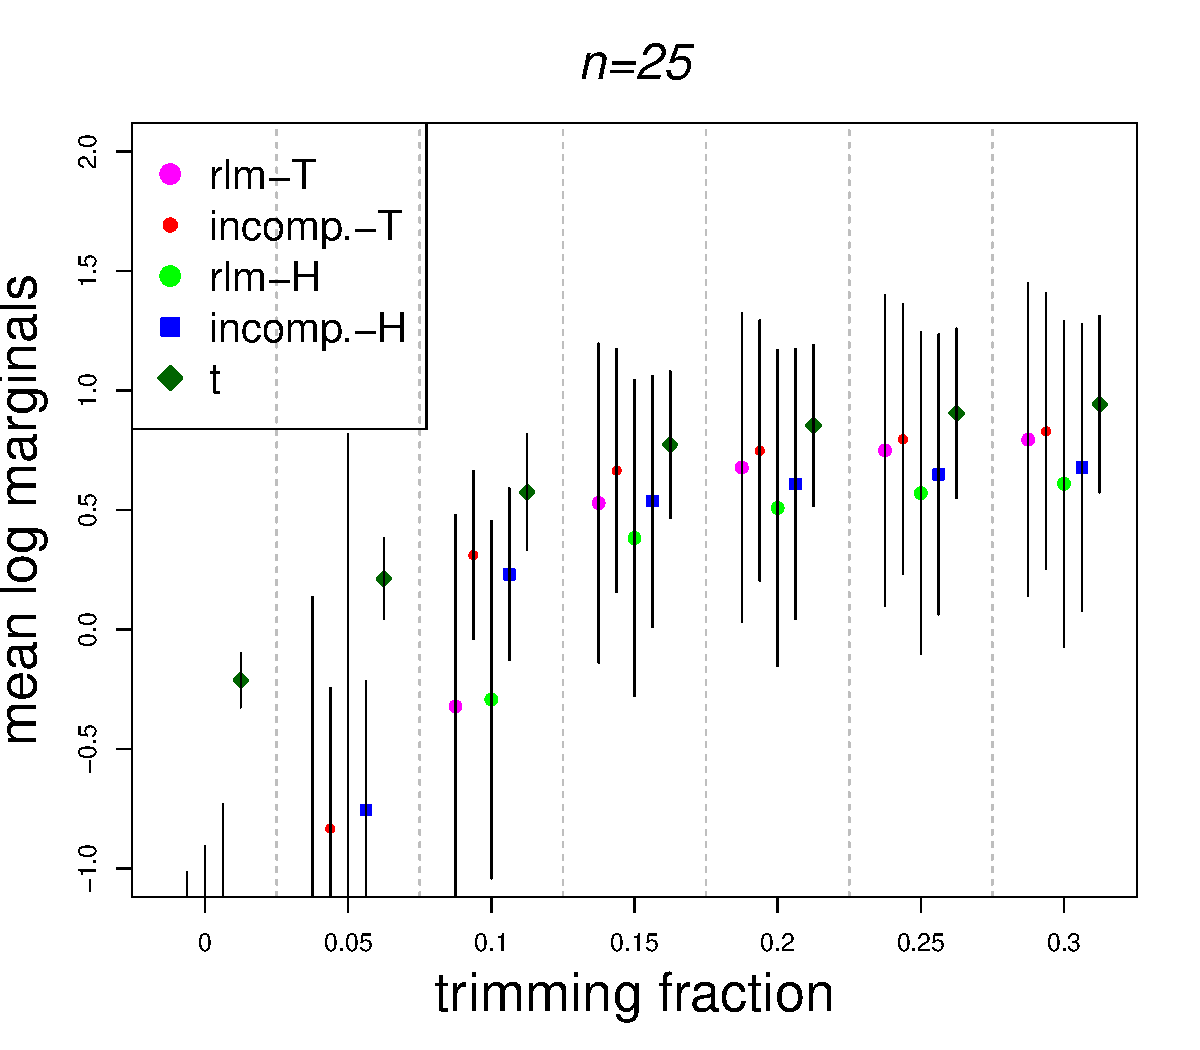
\includegraphics[width=3.4in,height=3.3in, page=1]{logMargType1AgenciesBaseModelt}}\quad
%\subcaptionbox{}{\includegraphics[width=3.4in,height=3.3in,page=2]{logMargType1AgenciesBaseModelt}}\quad
%\subcaptionbox{}{\includegraphics[width=3.4in,height=3.3in,page=3]{logMargType1AgenciesBaseModelt}}
%\caption{Model evaluation for `Type 1' agencies for training sample
%  sizes of $n=25,100$, and $1000$. The $t$-model is used as the base
%  method to compute TLM. Plotted are the mean TLM for each model
%  against the trimming fraction across the $100$ cross-validation
%  samples. Error bars correspond to one standard deviation of TLM
%  above and below the mean. Models are labeled with the following
%  abbreviations: `rlm' corresponds to a classical robust fit, `restr.'
%  corresponds to our restricted likelihood method, and `t' corresponds to the
%  heavy-tailed $t$-distribution model. The letters `T' and `H'
%  appearing after `rlm' and `restr.' correspond to the use of  Tukey's
%  and Huber's $\psi$ respectively.  
%}
%\label{fig:Type1Marg}
%\end{sidewaysfigure}
%


%Model evaluation for `Type 1' agencies is shown in Figure
%\ref{fig:Type1Marg} for training sample sizes $n=25, 100,$ and $1000$.
%The $t$-model is used as the base
%  method to compute TLM.
%The models pictured are: classical robust regression with Tukey's $\psi$ function (rlm-T), restricted likelihood with Tukey $\psi$ (restr.-T), classical robust regression with Huber's $\psi$ function (rlm-H), restricted likelihood  with Huber's $\psi$ (restr.-H), and the thick tailed $t$-model (t). The normal theory models perform poorly due to the numerous outliers
%and are left out of the figures. Appearing in the figures are the mean TLM across
%validations set for each model and each trimming fraction, $\alpha$ (along the $x$-axis). The error bars depicted are one standard deviation of the TLM above and below the mean.  The range of the vertical axis is chosen to enhance important features and as a result, some evaluation measures extend below this range. In particular, the restricted likelihood methods perform poorly if no trimming is done; reflecting that these methods are not intended to fit well to outliers. Recall that we expect about 15-16\% outliers in the validation sets, thus trimming fractions slightly larger than this amount are needed in order to assess fits to the `good' data. For $n=25$, the thick tailed model  prevails across trimming fractions, although less so for $\alpha\geq 0.15$. For sample sizes as low as $n=100$, the restricted likelihood methods outperform the heavy-tailed model with the Tukey version performing the best.   
%The stronger performance of restricted likelihood based on Tukey's method and the t model is to be expected, as many of the 
%residuals are so extreme that trimming is better than winsorizing (as Huber's method effectively does).  
%As expected, with enough data,  the Bayesian methods and their classical counterparts perform similarly, although there
%is a persistent slight edge in favor of the Bayesian restricted likelihood methods.  We attribute this advantage to the weakly informative
%prior distribution which pulls the estimates slightly toward better values.  The similarity occurs as early as $n=100$. 
%
 
\subsection{Hierarchical regression model}
\label{hierRegNW}
The previous analysis treated states independently. A natural extension is to  reflect similar business environments between states using a hierarchical regression. The proposed model is:
\begin{align}
%\begin{split}
\label{eq:hierModel}
&\bbeta\sim N_p(\bmu_0, a\Sigma_0);\ \ 
\bbeta_j\iid N_p(\bbeta, b\Sigma_0); \ \  
\sigma_j^2\sim IG(a_0,b_0);  & \\ 
& y_{ij}=\bx_{ij}^\top\bbeta_j+\epsilon_{ij},\ \ \epsilon_{ij}\iid N(0, \sigma_j^2),\ i=1,\dots, n_j,\ j=1,\dots, J &
%\end{split}
\end{align}
where $y_{ij}$ is the $i^{th}$ observation of square rooted household count in 2012 in the $j^{th}$
state, $n_{j}$ is the total number of agencies in state $j$, and $J$ is
the number of states. $\bx_{ij}$ is same tree-dimensions covariate vector as before and $\bbeta_j$ represents the individual regression coefficient vector for state $j$. The parameters $\bmu_0$,
$\Sigma_0$, $a_0$, and $b_0$ are fixed by fitting  the regression $y_{ij}=\bx_{ij}^{\top}\bbeta+\epsilon_{ij}$ using Huber's M-estimators to the prior data set from two years before. Using the estimates from this model, we set $\mu_{0} = \hat\beta$, $\Sigma_{0} = n_{p}\hat{\Sigma_{0}}$ ($n_{p} = 2996$ is the number of observations in the prior data set), $a_{0}=5$ and $b_{0} = \hat\sigma^{2}(a_{0} -1)$. We constrain $a+b=1$
in an attempt to partition the total variance between the individual
$\bbeta_j$'s and the overall $\bbeta$ and take $b\sim
\text{beta}(v_1,v_2)$. Using the prior data set, we assess the
variation between individual estimates of the $\bbeta_j$ to set $v_1$
and $v_2$ to allow for a reasonable amount of shrinkage. To allow for
dependence across the $\sigma_j^2$ we first take
$(z_1,\dots,z_J)\sim N_J(\mathbf{0}, \Sigma_\rho)$ with
$\Sigma_\rho=(1-\rho)\mb{I}+\rho \mb{1}\mb{1}^{\top}$. Then we set
$\sigma^2_j=H^{-1}(\Phi(z_j))$ where $H$ is the cdf of an
$IG(a_0,b_0)$ and $\Phi$ is the cdf of a standard normal. This results in the specified marginal distribution, while
introducing correlation via $\rho$. We assume $\rho\sim
\text{beta}(a_\rho,b_\rho)$ with mean $\mu_\rho=a_\rho/(a_\rho+b_\rho)$ and precision
$\psi_\rho=a_\rho+b_\rho$. The parameters $\mu_\rho$ and
$\psi_{\rho}$  are given beta and gamma distributions, with fixed hyperparameters. More details on setting prior parameters are given in the Supplementary Material. 

Using the same techniques as in the previous section, 
we fit the normal theory hierarchical model above, a thick-tailed $t$ version with $\nu = 5$ d.f., and two restricted likelihood versions (Huber's and Tukey's) of the model.  For the restricted methods, we condition on robust regression estimates fit separately within each state. We also fit classical robust regression counterparts and a least squares regression separately within each state. Hierarchical models naturally require more
data and so we include states having at least 25 agencies with sufficient variation within each covariate, resulting in 20 states in total and $n = \sum_{j} n_{j} =  3094$ total agencies. For training data we take a stratified (by state) sample of size $3094/2 = 1547$ where the strata sizes are $n_{j}/2$ (rounded to the nearest integer). The remaining data is used for a holdout evaluation using TLM computed separately within each state: $TLM_b(A)_{j} = (M_{j} - [\alpha M_{j}])^{-1} \sum_{i=[\alpha M_{j}]+1}^{M_{j}} \log(f_A(y_{(i)j}^b))$ where $y_{(1)j}^b, y_{(2)j}^b,..., y_{(M_{j})j}^b$ is the ordering of the $M_{j}$ holdout observations within state $j$ according to the log marginals under the base model $b$. For the non-Bayesian models,  $f_A(y^b_{(i)j})$ is estimated using plug-in estimators for the parameters for state $j$. $TLM_b(A)_{j}$ is computed for each state for $K=50$ splits of training and holdout sets. The Bayesian models are fit using MCMC, with the restricted versions applying the algorithm laid out in Section \ref{BayesLinMod} and adapted to the hierarchical setting as described in Section \ref{simData}. For the MH-step proposing augmented data,  \response{the acceptance rates for the two restricted likelihood models across all states and repetitions ranged from $0.01$ to  $0.75$, with only $7$ cases (out of 50*20*2 = 2000 chains) with rates below $0.1$}


The average over states, $\overline{TLM}_b(A)_{\cdot}= \frac{1}{22} \sum_{j =1}^{22} TLM_b(A)_{j}$ for each of the $K$ repetitions is summarized in Figure
\ref{fig:hierTLM} for several trimming fractions using the Student-t as the base model. The points are the average of the $\overline{TLM}_b(A)_{\cdot}$ over the $K$ repetitions with error bars plus/minus one standard deviation over $K$ with larger values representing better predictive performance. As the trimming fraction used for the TLM increases, so does TLM since more outliers are being trimmed. Similar patterns were seen in the individual state level regressions in Section \ref{regModelNW}. Despite being used as the base model to compute TLM, the Student-t doesn't perform well in comparison to the robust regressions. We attribute this to the assumption of heavier tails resulting in smaller log marginal values on average; emphasizing again that the t-model will do well to discount outlying observations but does not provide a natural mechanism for predicting non-outlying data. For each trimming fraction, our restricted likelihood hierarchical models outperform the classical robust regressions fit separately within each state. The hierarchical model also reduces variance in predictions resulting in smaller error bars. 

\begin{figure}[t]
\centering
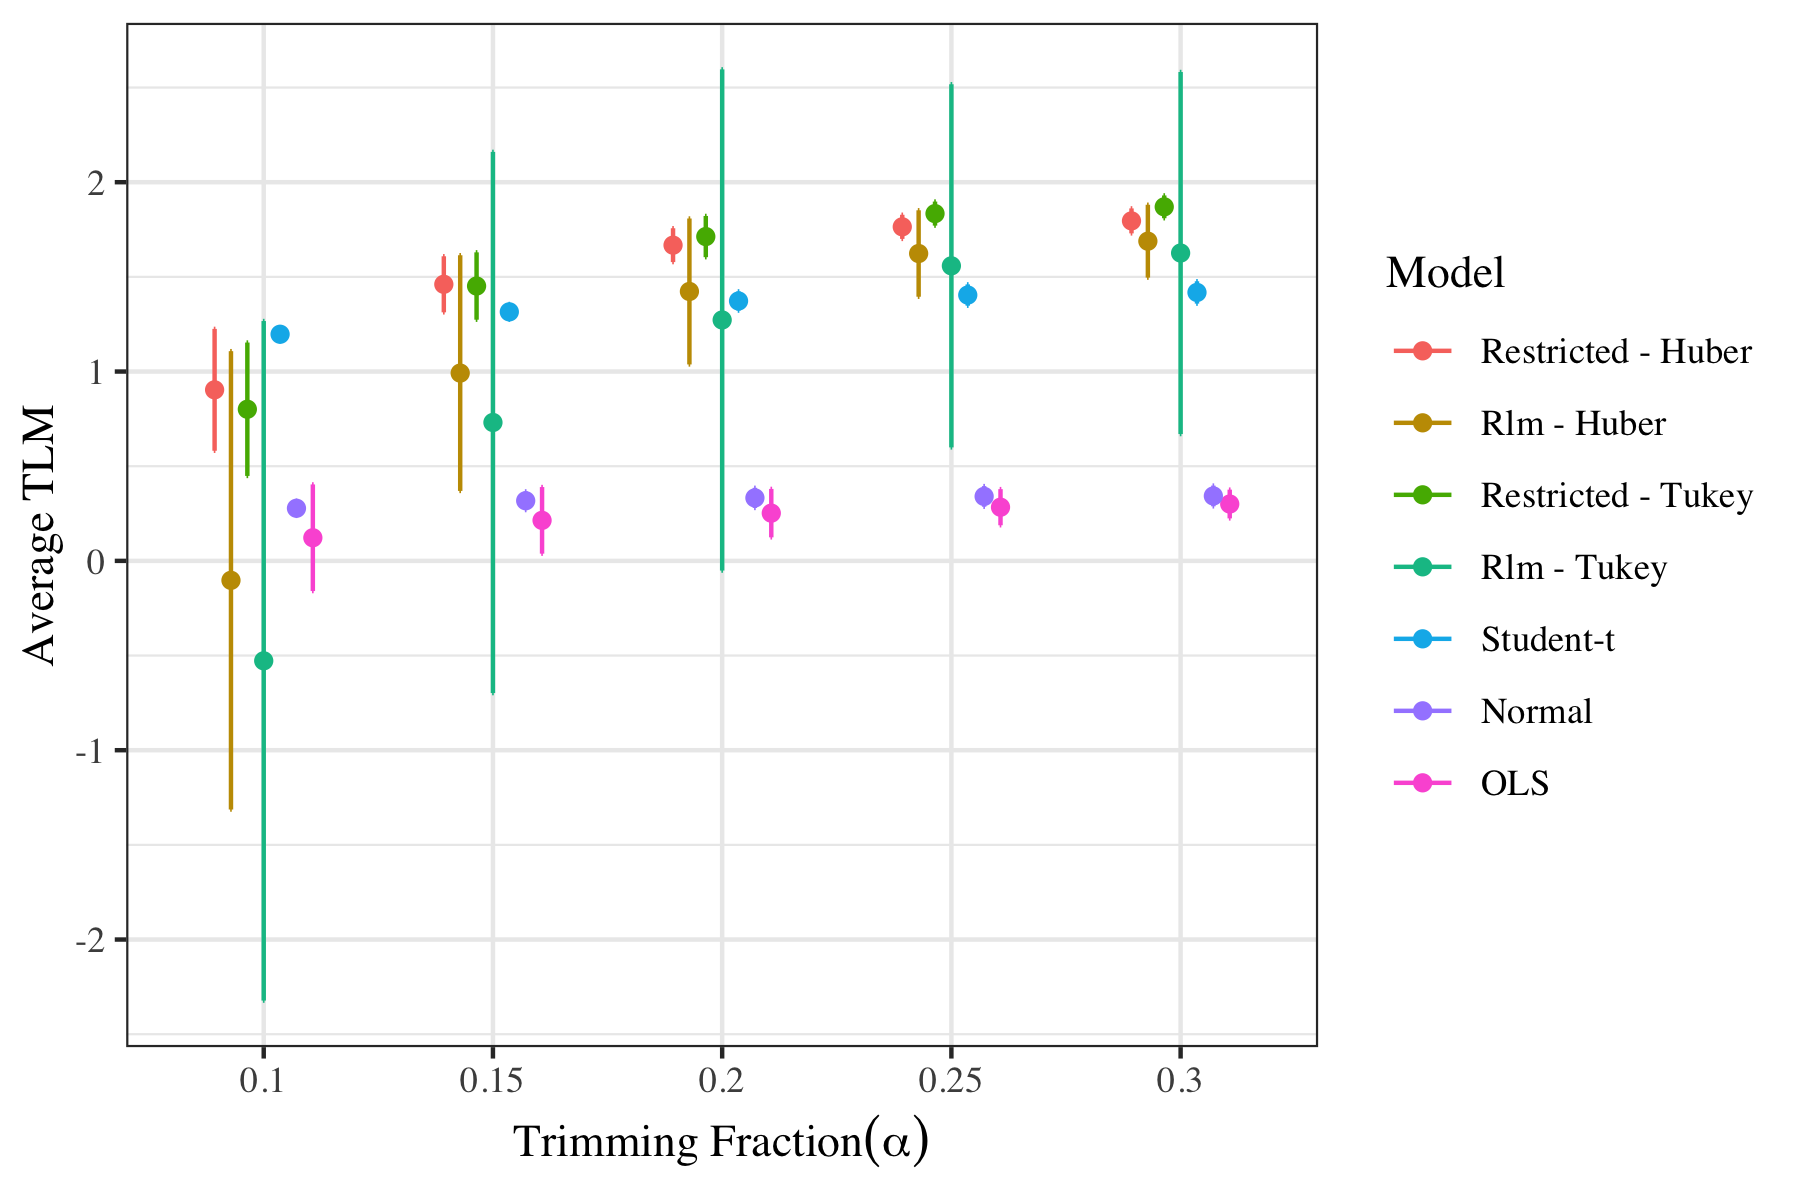
\includegraphics[width=6in]{hier_average_tlm.png}
\caption{Hierarchical model results: $\overline{TLM}_b(A)_{\cdot}$  plus/minus one standard deviation over $K = 50$ splits into training and holdout sets with the Student-t as the base model and several values of the trimming fraction $\alpha$. Larger values of TLM are better.}
\label{fig:hierTLM}
\end{figure}

%\begin{figure}[t]
%\centering
%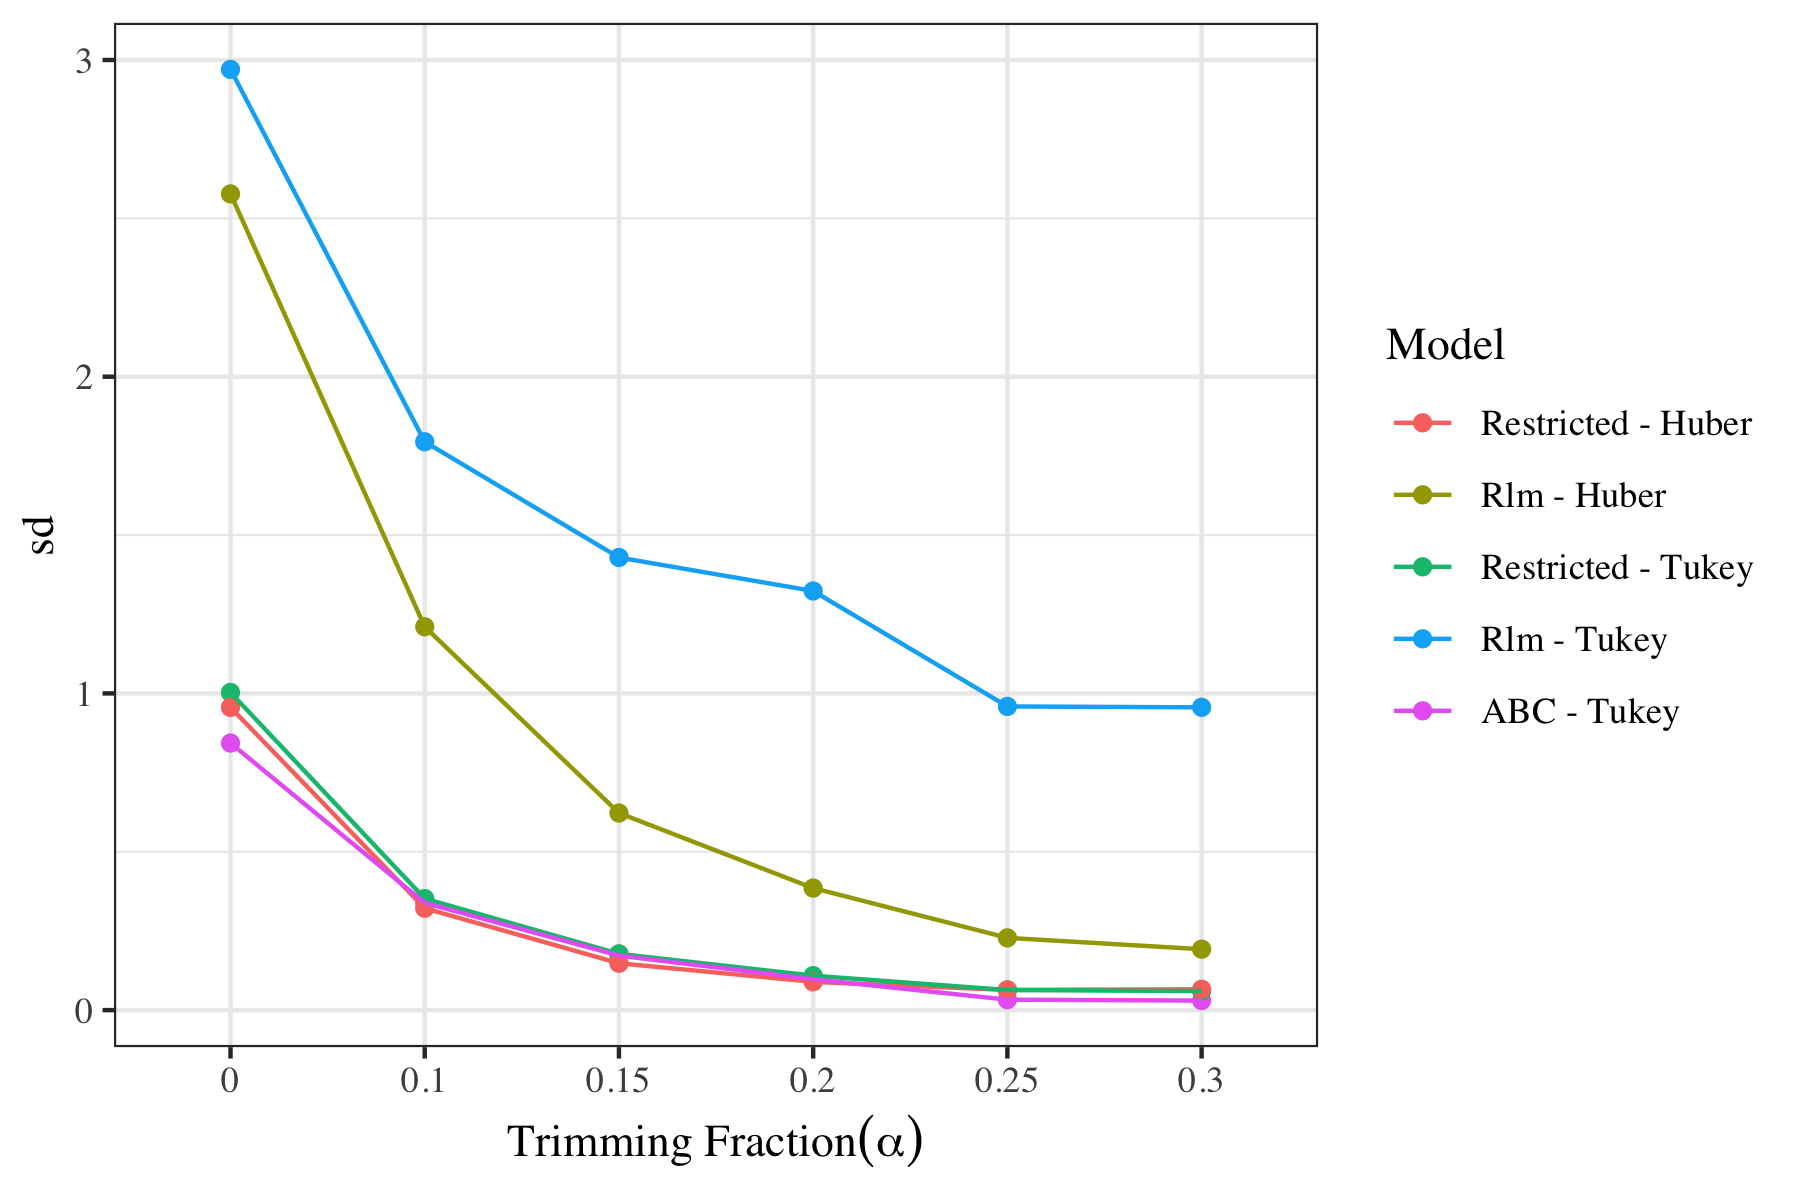
\includegraphics[width=6in]{hier_sd_tlm.png}
%\caption{Hierarchical model results: standard deviation of $\overline{TLM}_b(A)_{\cdot}$ relative to the mean over $K = 50$ splits into training and holdout sets for several values of the trimming fraction $\alpha$. Results are given for the two restricted likelihood versions of the hierarchical model and their corresponding robust regression models fit separately within each state.}
%\label{fig:hierTLMsd}
%\end{figure}

It is also interesting to examine the results within each state. Figure \ref{fig:hierTLMstate} summarizes ${TLM}_b(A)_{j}$ with $\alpha = 0.3$ for each state where the points and error bars are the averages and plus/minus one standard deviation of ${TLM}_b(A)_{j}$ over the $K = 50$ repetitions. The results are only given for the models using Tukey's M-estimators (Huber's version is qualitatively similar). The states are ordered along the $x$-axis according to number of agencies within the state (shown in parentheses). State 28 is removed from the figure as the error bars for the classical robust regression are excessively large and distort the comparison.  In several of the smaller states, the restricted hierarchical model performs better with similar performance between the models in most of the larger states, a reflection of the decreased influence of the prior.  The hierarchical structure pools information across states, improving performance in the smaller states. The standard deviations are smaller for the hierarchical model in smaller states than they are for the corresponding classical model.  In larger states, the standard deviations are virtually identical. Similar benefits are often seen for hierarchical models \citep[e.g.,][]{gelman2006}. 

 
\begin{figure}[t]
\centering
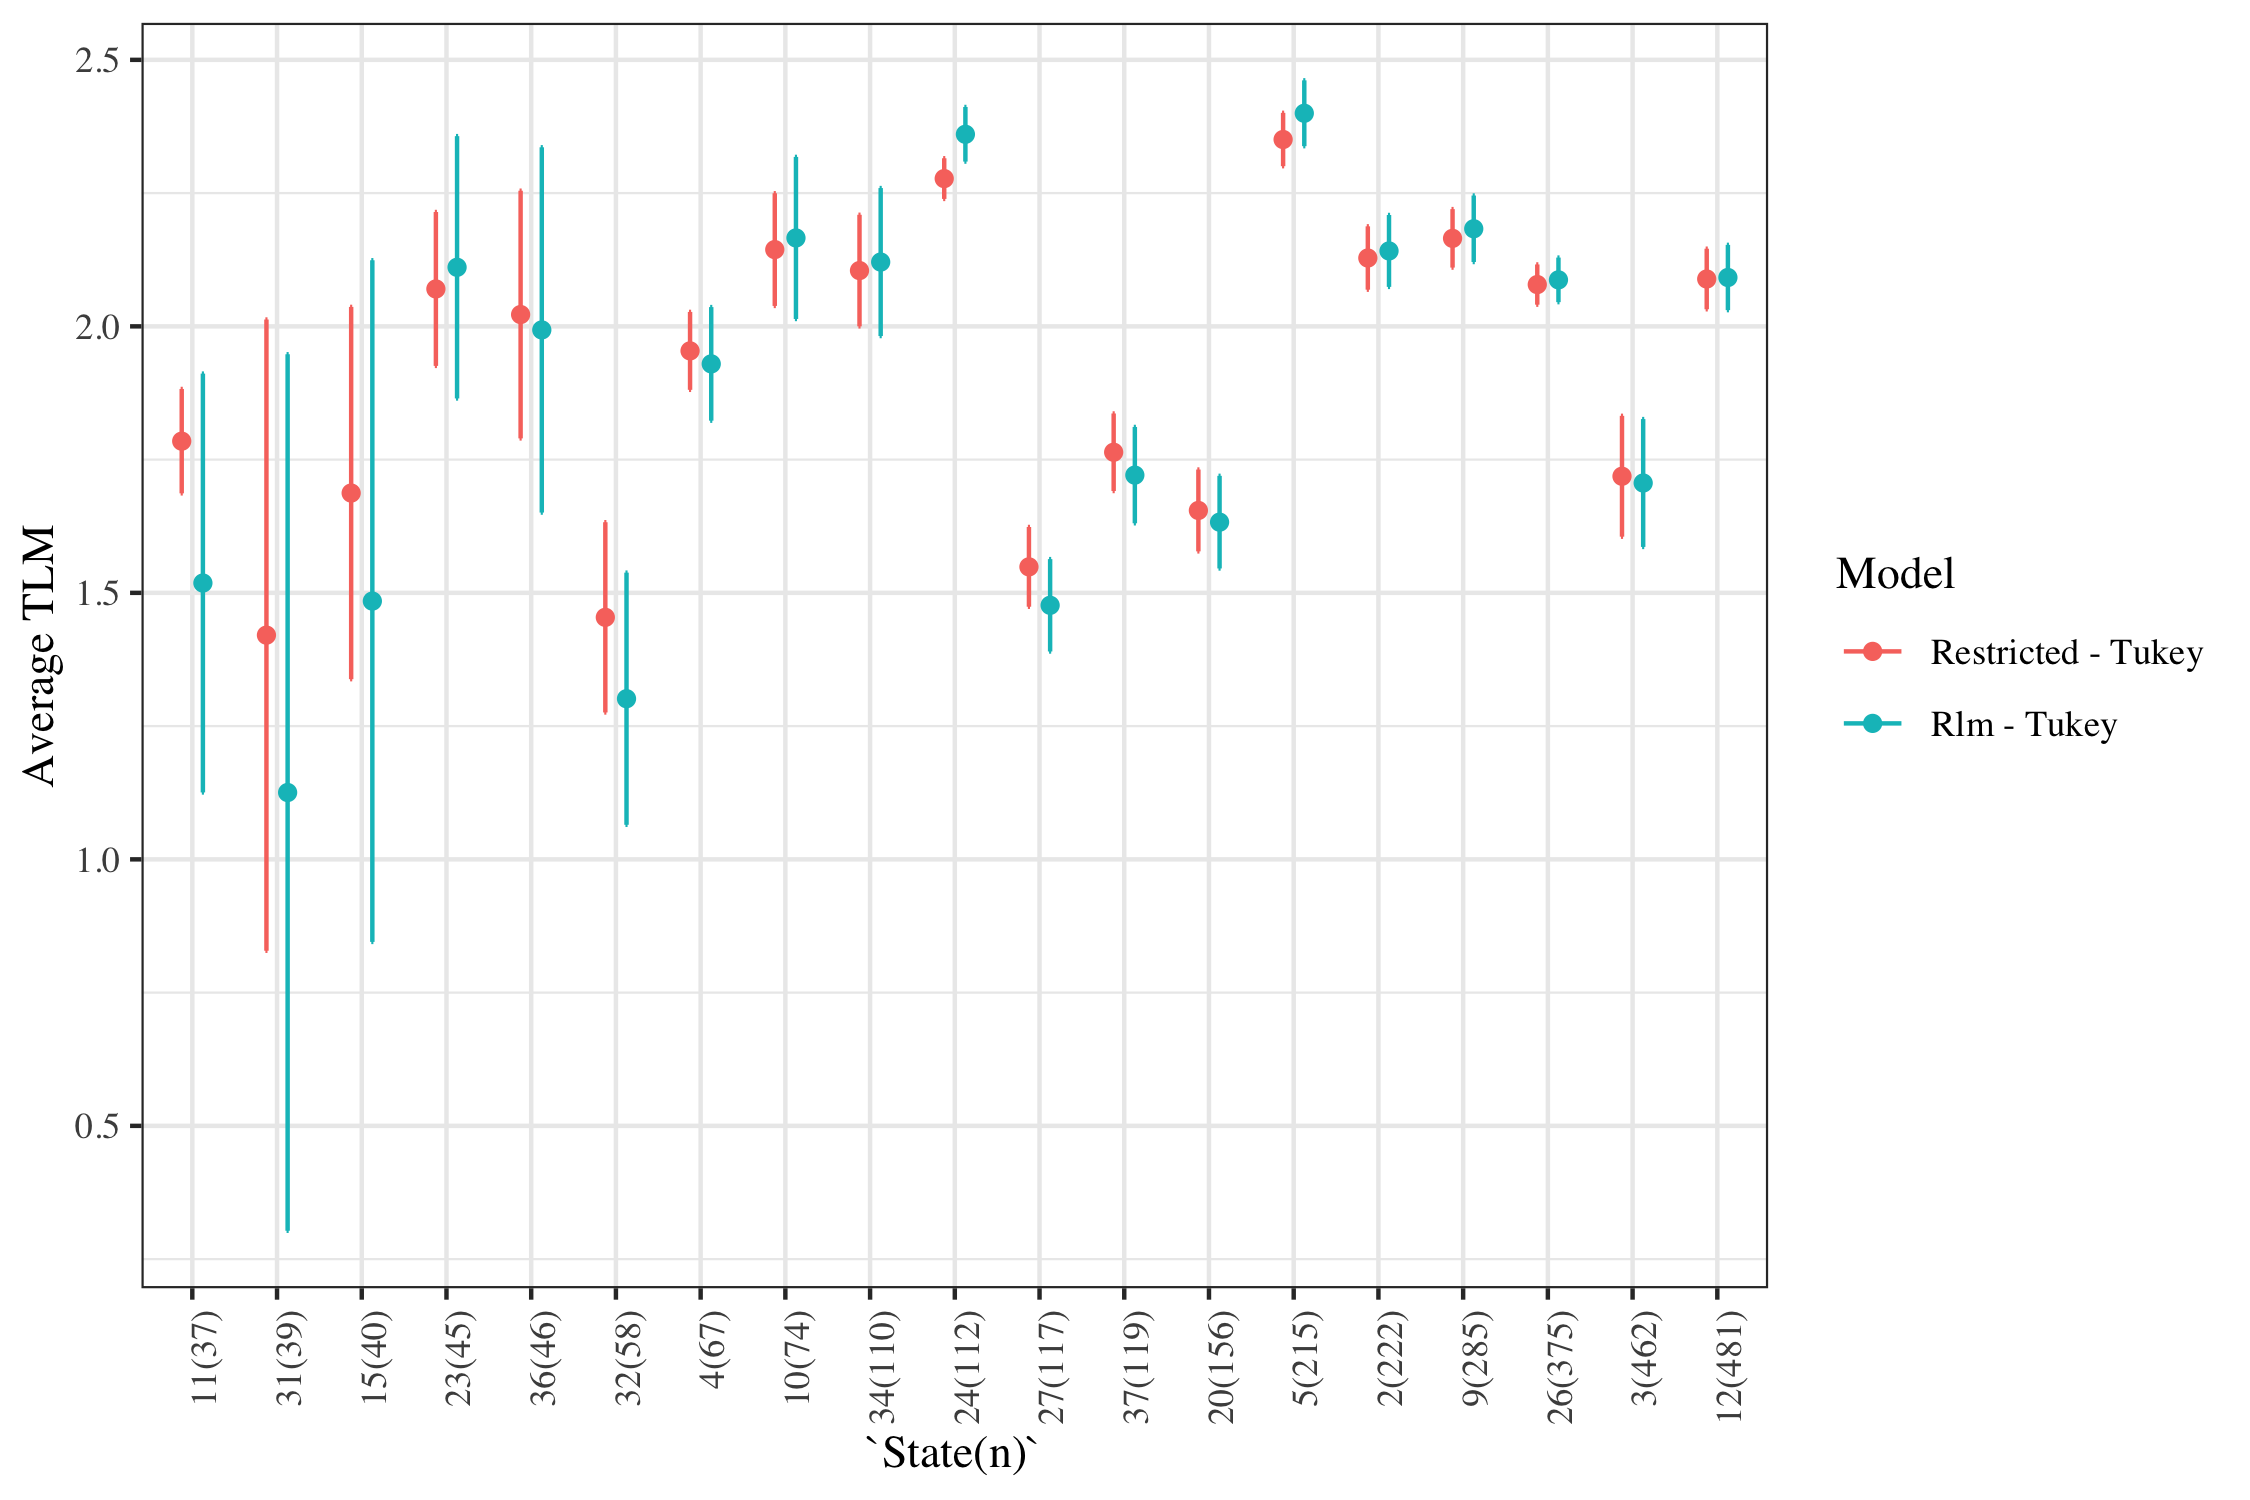
\includegraphics[width=6.8in]{hier_ave_tlm_state.png}
\caption{Hierarchical model results: ${TLM}_b(A)_{j}$  plus/minus one standard deviation over $K = 50$ repetitions for each state and $\alpha = 0.3$. The states are ordered along the $x$-axis according to number of agencies within the state (shown in parentheses). Results displayed are for the robust models using Tukey's M-estimators. Larger values of TLM are better.}
\label{fig:hierTLMstate}
\end{figure}

%\begin{figure}[t]
%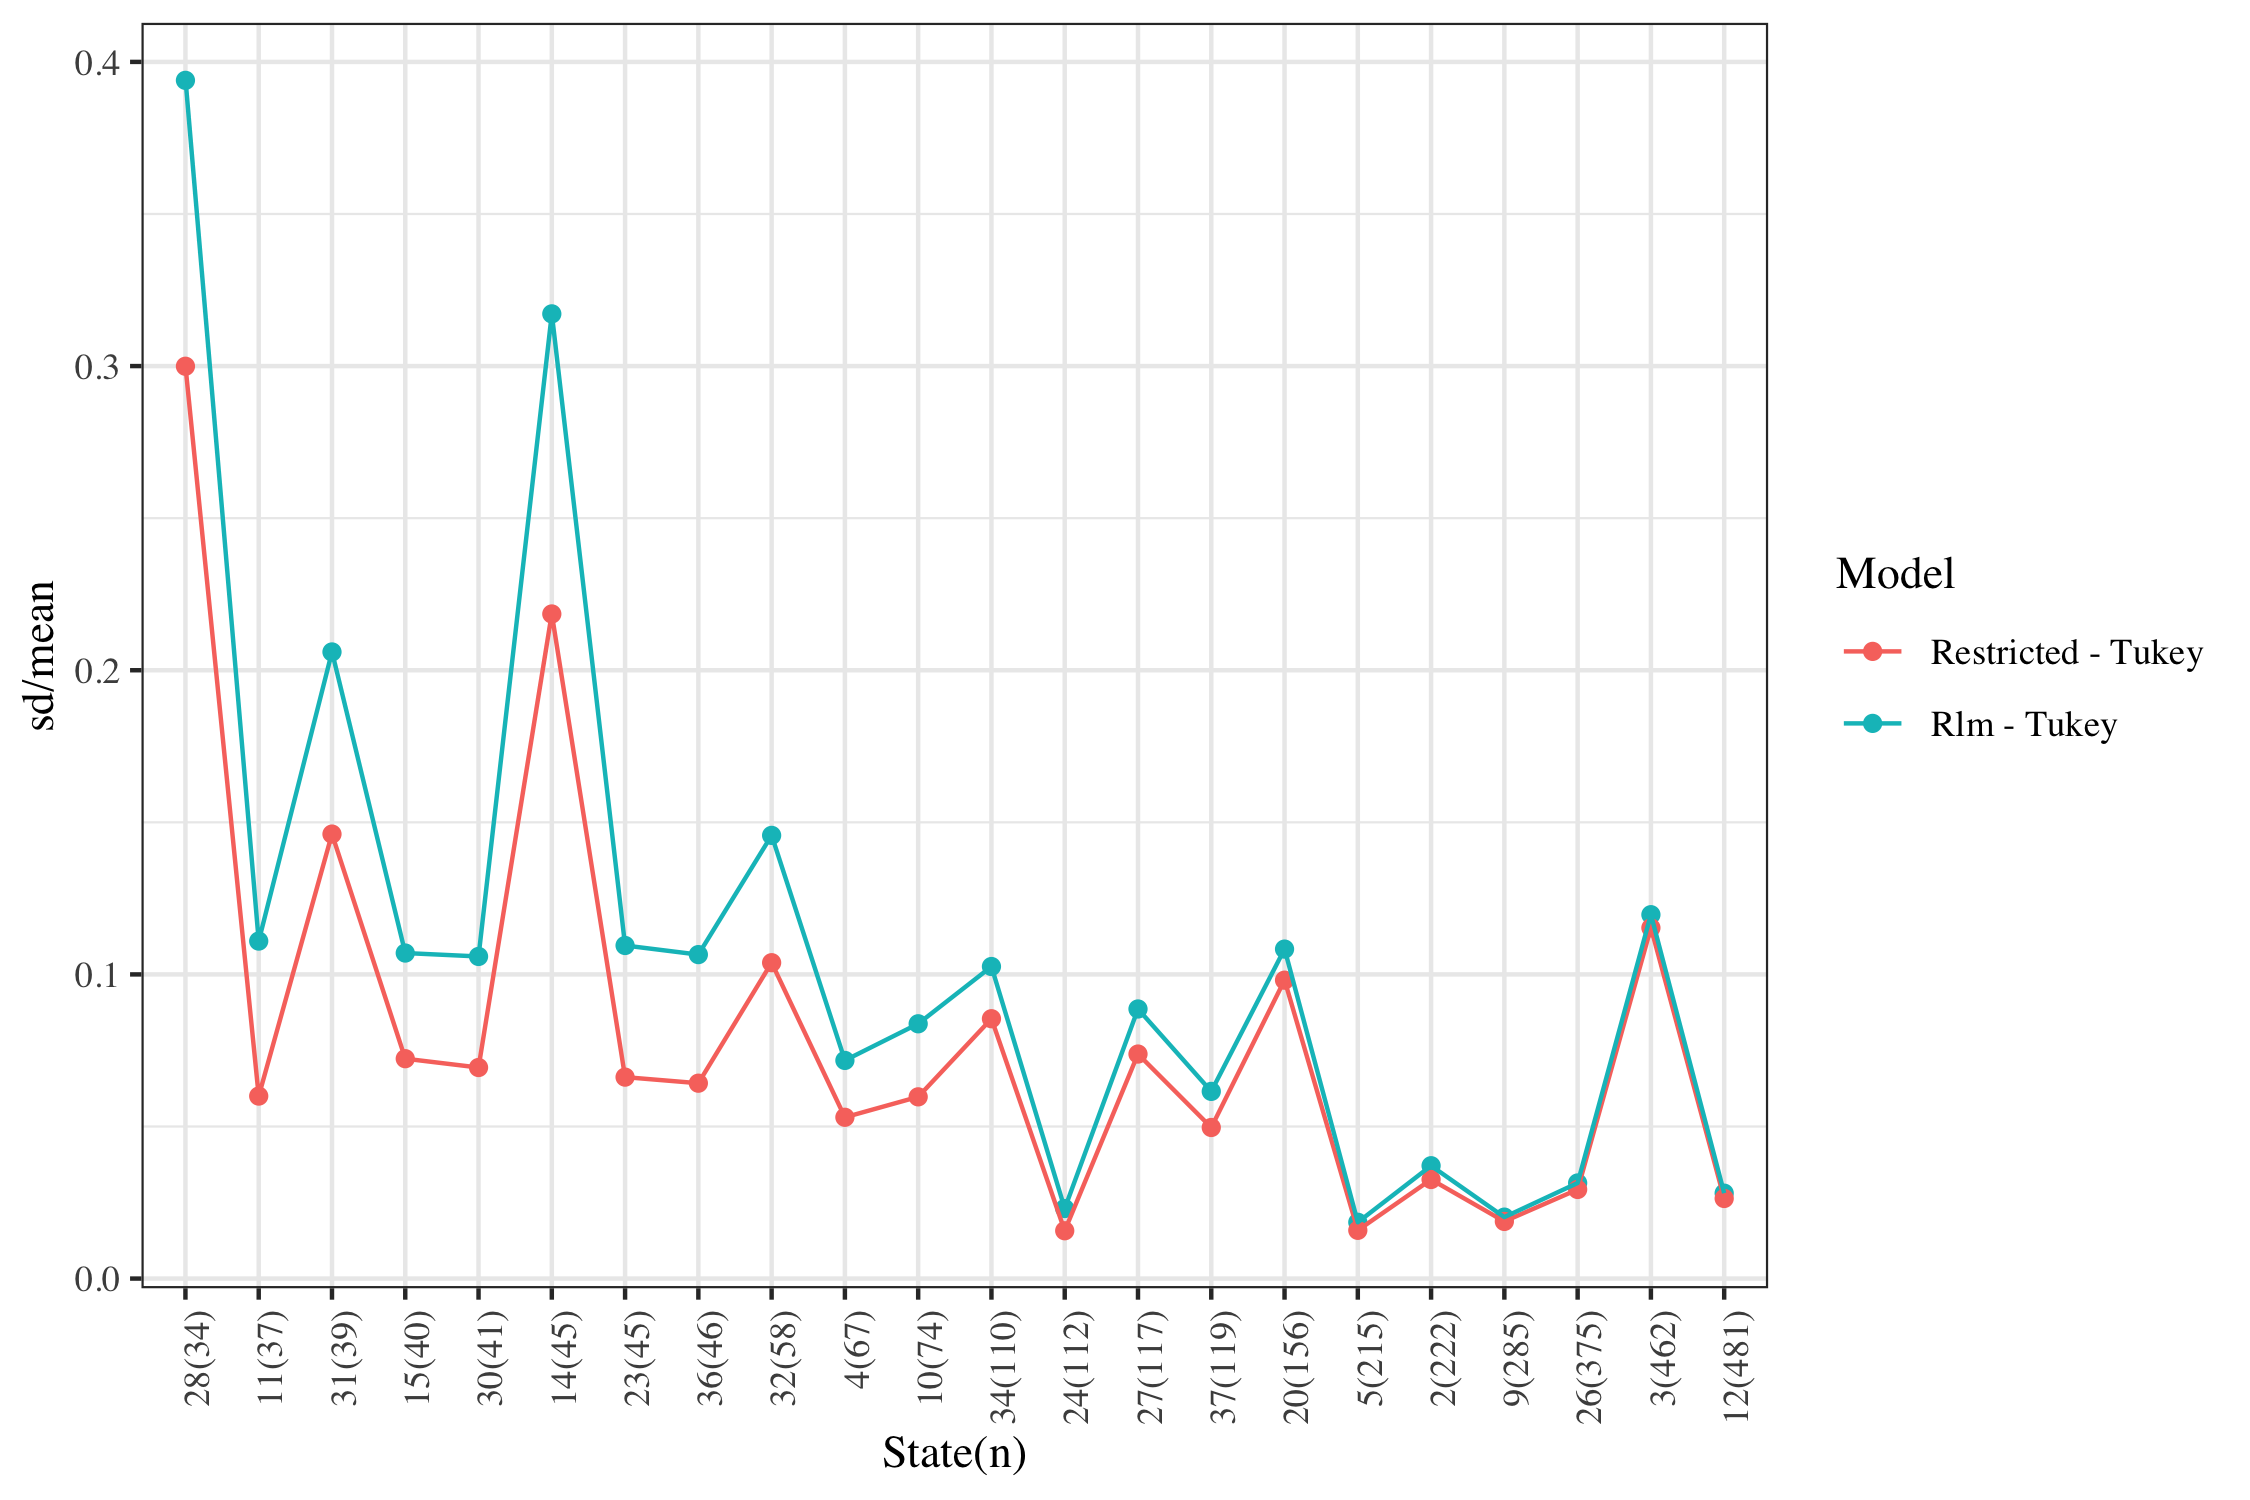
\includegraphics[width=7in]{hier_sd_tlm_state.png}
%\caption{Hierarchical model results: Standard deviation of ${TLM}_b(A)_{j}$  relative to the mean over $K = 50$ repetitions for each state and $\alpha = 0.3$. The states are ordered along the $x$-axis according to number of agencies within the state (shown in parentheses). Results displayed are for the robust models using Tukey's M-estimators.}
%\label{fig:hierTLMstateSD}
%\end{figure}



%We see that the restricted likelihood with Tukey's estimator performs best in each case (assuming sufficient trimming). Huber's version also tops the thick tailed model for $n=2000$.  The Bayesian restricted likelihood fits considerably outperform their respective individual classical robust fits for training size of $n=1000$. This observation remains, though marginally so, for $n=2000$. The advantage of the hierarchical models seen here is due to the pooling of information across states, resulting in better predictive performance as compared to both the thick tailed competitor as well the respective classical fits.



%\begin{sidewaysfigure}[t]
%%\subcaptionbox{}{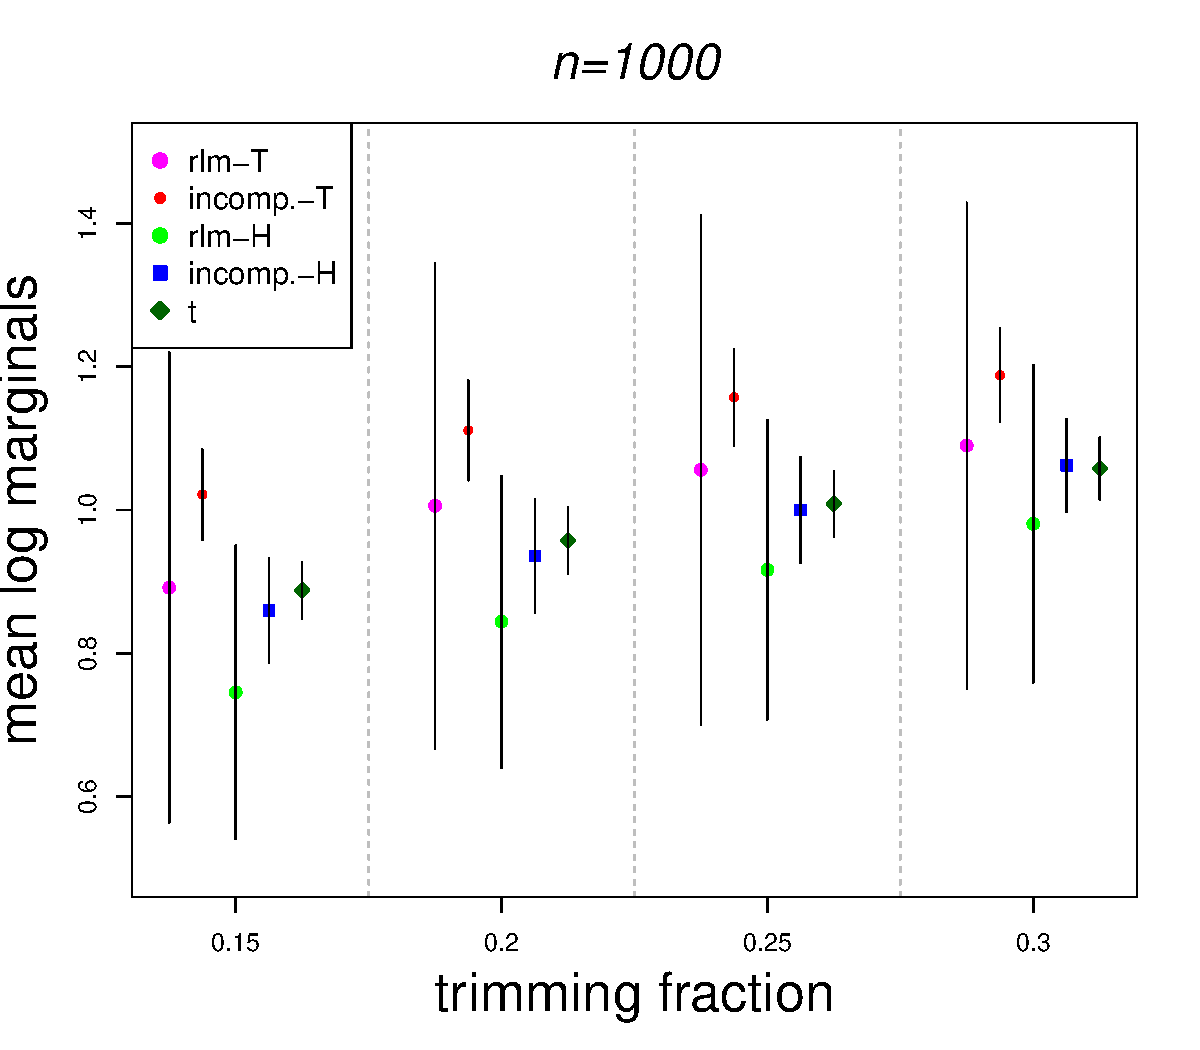
\includegraphics[width=2.75in,page=1]{hierlogMargType1AgenciesBaseModelt}}\quad
%%\subcaptionbox{}{\includegraphics[width=2.75in,page=2]{hierlogMargType1AgenciesBaseModelt}}
%\subcaptionbox{}{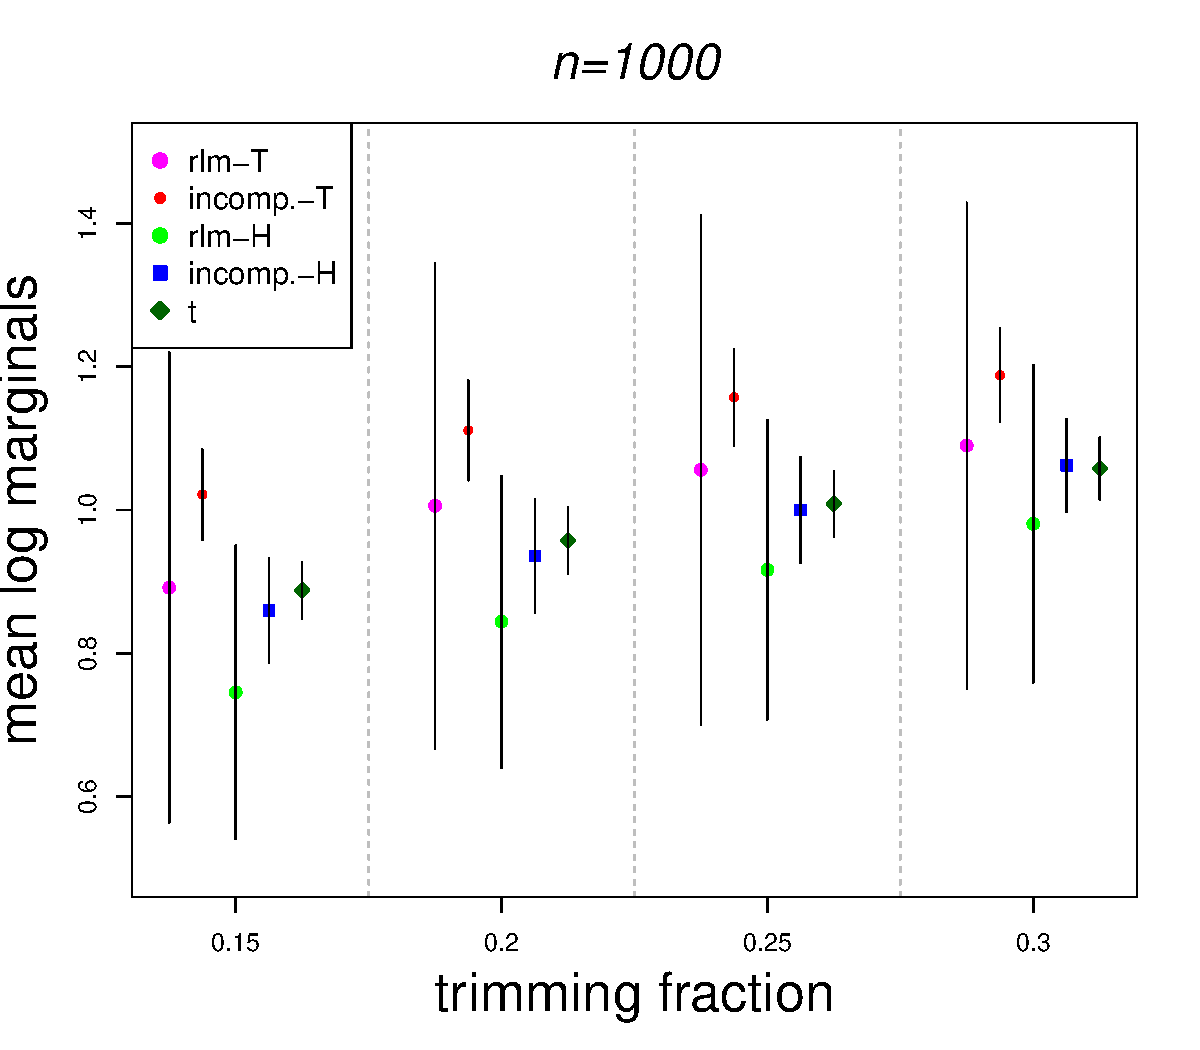
\includegraphics[width=4in,page=1]{hierlogMargType1AgenciesBaseModelt}}\quad
%\subcaptionbox{}{\includegraphics[width=4in,page=2]{hierlogMargType1AgenciesBaseModelt}}
%\caption{Model evaluation for `Type 1' agencies under the hierarchical model for $n=1000$ and $2000$. The $t$-model is used as the base method to compute TLM. Plotted are the mean TLM for each model against the trimming fraction across the $100$ cross-validation samples. Error bars correspond to one standard deviation of TLM above and below the mean. Models are labeled using the same notation as the previous figure. Only the relevant trimming fractions ($\alpha\geq .15$) are pictured.  
%}
%\label{fig:hierType1Marg}
%\end{sidewaysfigure}
%

%
%\subsection{Comparison of hierarchical and non-hierarchical fits}
%
%The performance of the methods for the hierarchical and non-hierarchical models can be contrasted through our cross validations studies.  We focus on Tukey's and Huber's conditioning statistic and concentrate our evaluation on the `Type 1' agencies. Table~\ref{tab:tlmTable} displays the mean TLM for each model and range of trimming fractions.  Our summary below focuses exclusively on realistic trimming fractions, $\alpha \geq 0.15$, and Tukey's conditioning statistic.  
%
%We first note that for the non-hierarchical model, there is little difference between mean TLM for $n=1000$ and $n=2000$, with 
%the numbers differing only in the third decimal place (see rows 1 and 3 of the table).  This is due to the posterior predictive distributions having stabilized.  The
%mean TLMs for the hierarchical model show a greater change with increases of about $0.05$ to $0.08$ as the training sample size changes
%from $1000$ to $2000$ (see rows 2 and 4 of the table).  For calibration, the mean TLM for a normal with mean $0.5$ and variance $1$ is approximately this size
%when trimming is done under a standard normal base model.  Thus, the increase in mean TLM is substantial.  
%We attribute the change for the hierarchical model to the 
%improvement in fits, particularly for states with fewer agencies.  
%
%Direct comparison of the hierarchical and non-hierarchical models shows that, for $n=1000$, the non-hierarchical model has uniformly 
%(for $\alpha$ of interest) better mean TLM (rows 1 and 2).  The differences are substantial, and the summaries primarily reflect greater stability of fits on a state-by-state basis under the non-hierarchical model.  To a lesser extent, they reflect variation in the evaluation criterion which stems from modest validation sample size, particularly with larger trimming fractions.  The trimmed cases are not proportionally distributed across states.  The pattern changes for $n=2000$ (rows 3 and 4), with the hierarchical model showing larger mean TLMs for trimming fractions $0.15$ and $0.20$.  The improvement reflects the ability of the hierarchical model to capture differences in regressions across the states which is realized when the training sample size is large enough.  We attribute the better performance of the non-hierarchical model for the largest trimming fractions to variation in the evaluation.  
%
%\begin{table}[!tbp]
%{\small
%\begin{center}
%\begin{tabular}{lllll}
%\hline\hline
%& \multicolumn{4}{c}{Trimming fraction ($\alpha$)}\\
%\multicolumn{1}{l}{}&\multicolumn{1}{c}{$0.15$}&\multicolumn{1}{c}{$0.2$}&\multicolumn{1}{c}{$0.25$}&\multicolumn{1}{c}{$0.3$}\tabularnewline
%\hline
%{\mdseries Tukey ($n=1000$)}&&&&\tabularnewline
%~~Non-Hier.&1.072 (0.014)&1.179 (0.022)&1.226 (0.029)&1.255 (0.033)\tabularnewline
%~~Hier.&1.021 (0.063)&1.110 (0.070)&1.157 (0.067)&1.187 (0.065)\tabularnewline
%\hline
%{\mdseries Tukey ($n=2000$) }&&&&\tabularnewline
%~~Non-Hier.&1.068 (0.029)&1.178 (0.007)&1.225 (0.011)&1.254 (0.014)\tabularnewline
%~~Hier.&1.094 (0.041)&1.189 (0.036)&1.221 (0.033)&1.242 (0.028)\tabularnewline
%\hline
%{\mdseries Huber  ($n=1000$)}&&&&\tabularnewline
%~~Non-Hier.&1.020 (0.020)&1.114 (0.035)&1.157 (0.041)&1.184 (0.045)\tabularnewline
%~~Hier.&0.861 (0.073)&0.937 (0.079)&1.001 (0.074)&1.063 (0.064)\tabularnewline
%\hline
%{\mdseries Huber ($n=2000$)}&&&&\tabularnewline
%~~Non-Hier.&1.015 (0.021)&1.112 (0.014)&1.154 (0.019)&1.181 (0.023)\tabularnewline
%~~Hier.&0.930 (0.041)&1.014 (0.043)&1.080 (0.035)&1.148 (0.027)\tabularnewline
%\hline
%\end{tabular}
%\end{center}
%\caption{Mean (standard deviation) of TLM for `Type 1' agencies for the Bayesian restricted likelihood non-hierarchical and hierarchical models for $n=1000$ and $2000$.} \label{tab:tlmTable}
%}
%\end{table}
%

\section{Discussion}
\label{Conclusions}

This paper develops a Bayesian version of restricted likelihood where posterior inference is conducted by conditioning on a summary statistic rather than the complete data.  The framework blends classical estimation with Bayesian methods.  
%Many routine choices in an analysis react to the gap between reality and the
%statistical model, where a bit of set-up work improves inferential
%performance.  Often, these choices can be recast in the framework of
%restricted likelihood presented here, lending them more formality and facilitating
%development of theoretical results. 
%A greater benefit of our framework is that it leads us to blend classical estimation with Bayesian methods. 
Here, we concentrate on outlier-prone settings where natural choices for the conditioning statistic are classical robust estimators targeting the mean of the non-outlying data (e.g., M-estimators).  The likelihood conditioned on these estimators is used to move from prior to posterior. The update follows Bayes' Theorem, conditioning on the observed estimators exactly.   Computation is driven by MCMC methods, requiring only a supplement to existing algorithms by adding a Gibbs step to sample from the space of data sets satisfying the observed statistic. This step has additional computation costs arising from the need to compute the estimator and an orthonormal basis derived from gradients of the estimator at each iteration. The cost of finding the basis can be reduced by exploiting properties of the geometric space from which the samples are drawn as described in Section~\ref{highDim}. We have seen good mixing of the MCMC chains across a wide-variety of examples. %\response{We have found the additional computational burden to be beneficial in situation where  substantial prior information that will impact the results is available.}
\response{We have found the benefits of using our Bayesian technique to outweigh the additional computational burden (relative to a classical estimator) in the situation where substantive prior information that will impact the results is available.}
 
The Bayesian restricted likelihood framework can be used to address model misspecification, of which the presence of outliers is but one example. The traditional view is that, if the model is inadequate, one should build a better model. In our empirical work, as data sets have become larger and more complex, we have bumped into settings where we cannot realistically build the perfect model. We ask the question ``by attempting to improve our model through elaboration, will the overall performance of the model suffer?'' If yes, we avoid the elaboration, retaining a model with some level of misspecification. Acknowledging that the model is misspecified implies acknowledging that the sampling density is incorrect, exactly as we do when outliers are present. In this sense, misspecified models and outliers are reflections of the same phenomenon, and we see restricted likelihood as a method for dealing with this more general problem. 

Outside of outlier-prone settings, we might condition on the results of a set of estimating equations designed to enforce a lexical preference for those features of the analysis considered most important, yet still producing inferences for secondary aspects of the problem. This leads to questions regarding the choice of summary statistic to apply. In the literature, great ingenuity has been used to create a wide variety of estimators designed to handle specific manifestations of a misspecified model.  The estimators are typically accompanied by asymptotic results on consistency and limiting distribution.  These results can be used as a starting point to choose appropriate conditioning statistics in specific settings.  For example, a set of regression quantiles may be judged the most important feature of a model.  It would then be natural to condition on the estimated regression quantiles and to use a flexible prior distribution to allow for nonlinearities in the quantiles.  The computational strategies we have devised allow us to apply our methods in this setting and to make full predictive inference.  In general, we recommend a choice of conditioning statistic based on the analyst's understanding of the problem, model, reality, deficiencies in the model,  inferences to be made, and the relative importance of various inferences.  

The framework we develop here allows us to retain many benefits of Bayesian methods:  it requires a complete model for the data; it lets us combine various sources of information both through the use of a prior distribution and through creation of a hierarchical model; it guarantees admissibility of our decision rules among the class based on the summary statistic $T(\by)$; and it naturally leads us to focus on predictive inference.  The work does open a number of questions for further work, including a need to investigate restricted likelihood methods as they relate to model selection, model averaging for predictive performance, and model diagnostics. 




%Perhaps the biggest question is which summary statistic to choose.  For this, we recommend a choice based on the analyst's understanding of the problem, model, reality, deficiencies in the model,  inferences to be made, and the relative importance of various inferences.  \green{In our words, to provide desireable inference, we recommend use of robust and relevant summary statistics in conjunction with Bayesian models.}  


\section{Supplementary Material}
\label{sec:appendix}

\subsection{Practical Considerations for Using the Restricted Likelihood}
We offer the following guidelines and recommendations for using these methods in practice. 
\begin{itemize}
\item We have shown the method to be useful in outlier prone situations where good prior information can be encoded for the `good' part of the model. The additional computation burden may be too much when this is not the case. Traditional robust estimation techniques are often quicker and can provide comparable results.
\item Currently, we recommend conditioning on classical robust estimators when using these methods. Examples include Huber's and Tukey's estimators as outlined in the paper. We have found default choices (e.g. obtaining 95\% efficiency under normally distributed data) for the tuning parameters to work well in many situations. However, depending on the amount of contamination, some adjustment may be necessary. 
\item The likelihood itself can indeed take many forms and, like the conditioning statistic, can depend on the application. We have developed methods for fitting these models under a large class of conditioning statistics. In outlier prone situations we have had success using a normal likelihood model, with the conditioning intended to reduce the sensitivity of the analysis to the outliers. 
\item Comparisons amongst various choices of conditioning statistics and models can be made via standard cross-validation techniques like those done in this paper where models are fit to several training and holdout sets. One should take care in the method of evaluation. When the goal is to obtain good estimation/prediction for the non-outlying data, evaluation should take place on non-outlying data or the metric should be adjusted to discount outlying data ins some way (such as the trimmed-log-marginal we introduced TLM).
\end{itemize}

%\subsection{An Additional Illustrative Example}


%As a second example, a data set measuring the number of telephone calls in Belgium from 1950-1973 is analyzed. The outliers in this case are due to a change in measurement units on which calls were recorded for part of the data set. Specifically, for years 1964-1969 and parts of 1963 and 1970, the length of calls in minutes were recorded rather than the number of calls \citep{rousseeuw1987}. The full model is a standard normal Bayesian linear regression:
%\begin{equation}
%{\boldsymbol{\beta}}\sim N_{2}(\boldsymbol{\mu}_{0}, \boldsymbol{\Sigma}_{0}),\  \sigma^{2} \sim IG(a, b),\  \by \sim N(X\boldsymbol{\beta}, \sigma^{2} I),
%\end{equation}
%where $\bbeta = (\beta_{0}, \beta_{1})^{\top}$, $\by$ is the vector of the logarithm of the number of calls, and $X$ is the $n\times 2$ design matrix with a vector of 1's in the first column and the year covariate in the second.  Prior parameters are fixed via a maximum likelihood fit to the first 3 data points. In particular, the prior covariance for $\bbeta$ is set to $\Sigma_{0} = g\sigma_{0}^2 (X_{p}^{\top}X_{p})^{-1}$, with $X_{p}$ the $3\times 2$ design matrix for the first $3$ data points, $g=n=21$, $\sigma_{0} = 0.03$ and $\boldsymbol{\mu}_{0} = (1.87,  0.03)^{\top}$.  This has the spirit of a unit information prior \citep{kass1995reference} but uses a design matrix for data not used in the fit. Finally $a = 2$ and $b =1$.
%
%Four models are compared: 1) the normal theory base model 2) a two component normal mixture model, 3) a t-model, and 4) a restricted likelihood model conditioning on Tukey's M-estimator for the slope and intercept with Huber's `proposal 2'  for scale. Each model is fit to the remaining 21 data points. The normal theory model is also fit a second time after removing observations 14-21 (years 1963 - 1970). The omitted cases consist of the obvious large outliers as well as the two smaller outliers at the beginning and end of this sequence of points caused by the change in measurement units. The mixture model allows different mean regression functions and variances for each component.  Both components have the same, relatively vague priors. The probability of belonging to the first component is given a $\text{beta}(5,1)$ prior. The heavy-tailed model fixes the degrees of freedom at 5 and uses the same prior on $\bbeta$.  The prior on $\sigma^2$ is adjusted by a scale factor of $3/5$ to provide the same prior on the variance.  
%
%The data and  $95\%$ credible bands for the posterior predictive distribution under each model are displayed in Figure \ref{fig:calls_predictive}. The normal model fit to all cases results in a very wide posterior predictive distribution due to an inflated estimate of the variance. The t-model provides a similar predictive distribution.  The pocket of outliers from 1963 to 1970 overwhelms the natural robustness of the model and leads to wide prediction bands.  The outliers, falling toward the end of the time period, lead to a relatively high slope for the regression.  In contrast, the normal theory model fit to only the good data results in a smaller slope and narrower prediction bands.  The predictive distribution under the restricted likelihood approach is much more precise and is close to that of the normal theory fit to the non-outlying cases. The two component mixture model provides similar results, where the predictive distribution is formulated using only the good component. For these data, the large outliers are easily identified as following a distinct regression, leaving the primary component of the mixture for non-outlying data.  In a more complex situation where the outlier generating mechanism is transient (i.e., ever changing and more complex than for these data), modeling the outliers is more difficult. As in classical robust estimation, the restricted likelihood approach avoids explicitly modeling the outliers. 
%\begin{figure}[t]
%\centering
%{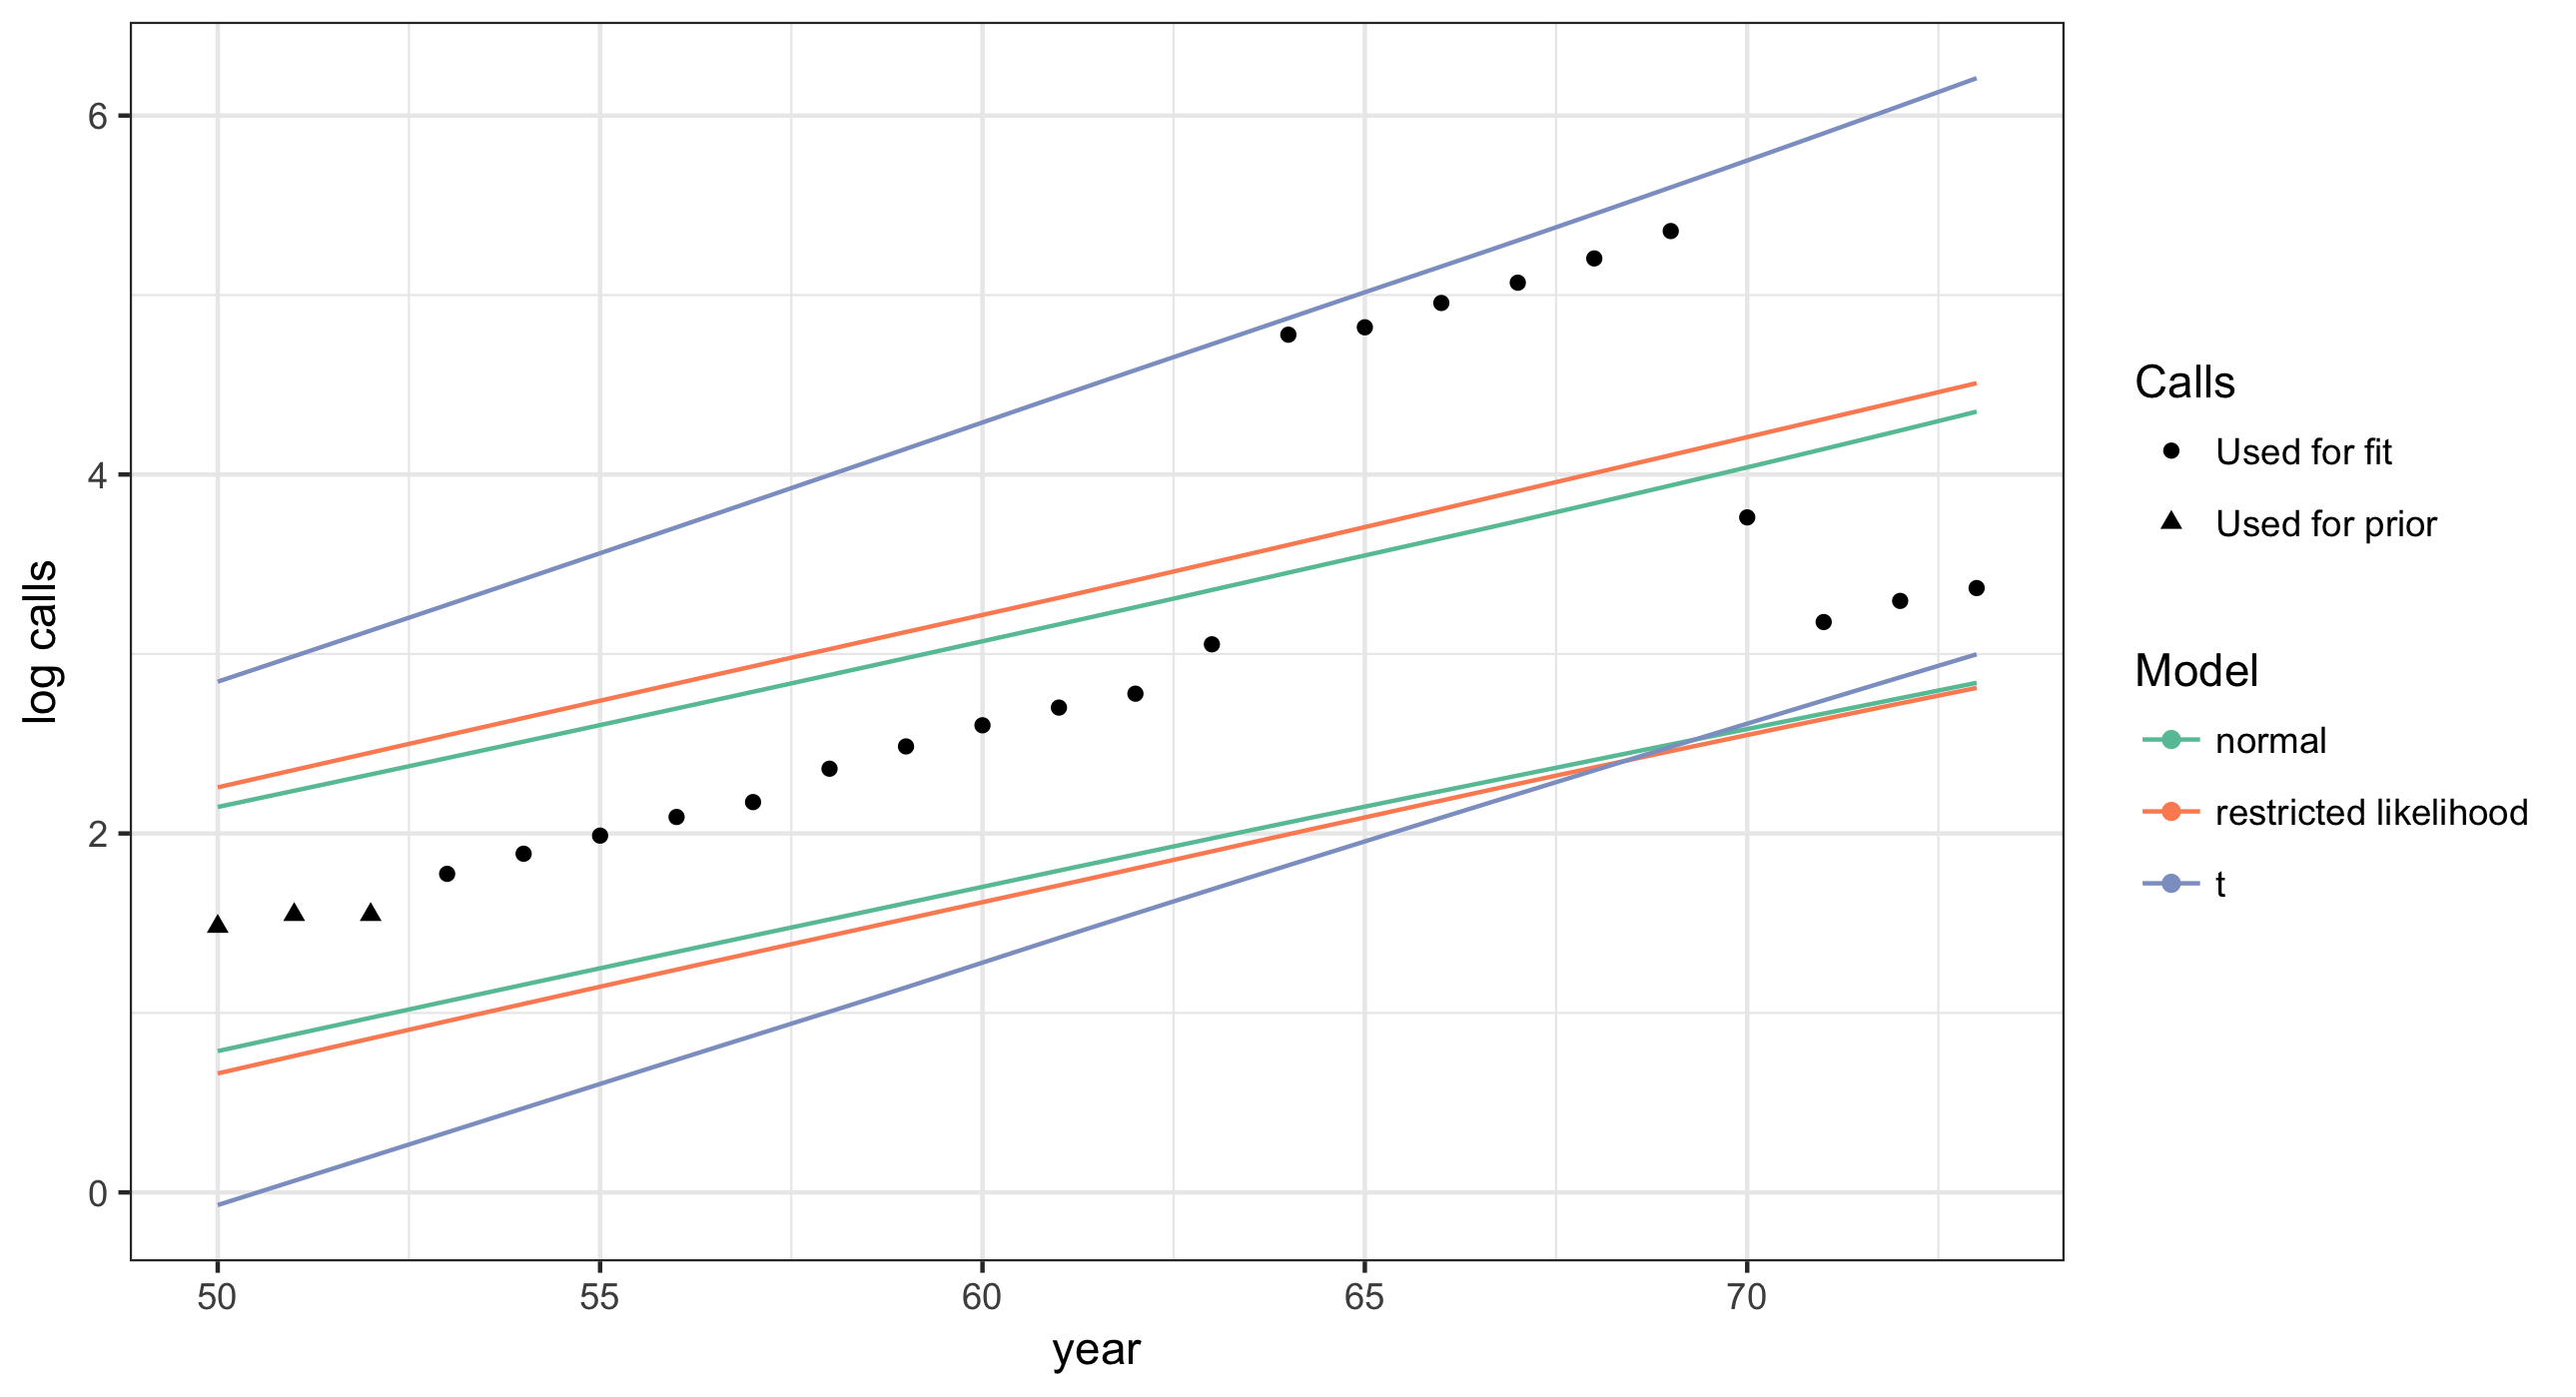
\includegraphics[width = 4in]{figs/calls_predictive.png}}
%\caption{Pointwise posterior predictive intervals of log(calls) under the normal theory model fit to the non-outliers, the restricted likelihood model with Tukey's M-estimator for the slope and intercept with Huber's `proposal 2'  for scale, and a heavy-tailed t-distribution model. The first three data points were used to specify the prior with each model using the remaining 21 for fitting. The normal theory model was also fit after removing observations 14-20 (years 1963 - 1970).}
%\label{fig:calls_predictive}
%\end{figure}
%
%

\subsection{Proofs}
\noindent

Proof of Theorem~\ref{Transformation}.  
\begin{proof} 
\begin{eqnarray}
 s(X,\by) & = & s\left(X,\frac{s(X,\by_{obs})}{s(X,\bz^*)}\bz^* + X\left(\bb(X,\by_{obs}) - \bb(X,\frac{s(X,\by_{obs})}{s(X,\bz^*)}\bz^*)\right)\right) \\
& = & \frac{s(X,\by_{obs})}{s(X,\bz^*)} s(X, \bz^*)= s(X,\by_{obs}) , \qquad \mbox{and} \\
 \bb(X,\by) & = & \bb\left(X,\frac{s(X,\by_{obs})}{s(X,\bz^*)}\bz^* + X\left(\bb(X,\by_{obs}) - \bb(X,\frac{s(X,\by_{obs})}{s(X,\bz^*)}\bz^*)\right)\right) \\
 & = & \bb(X,\frac{s(X,\by_{obs})}{s(X,\bz^*)}\bz^*) + \bb(X,\by_{obs}) - \bb(X,\frac{s(X,\by_{obs})}{s(X,\bz^*)}\bz^*) \\ &=& \bb(X,\by_{obs})
\end{eqnarray}
\end{proof}

\noindent
\begin{theorem}
\label{1to1onto}
The mapping $h:  \mathbb{S} \rightarrow \mathcal{A}$ with $h$ defined in Theorem \ref{Transformation} is one-to-one and onto. 
\end{theorem}
\begin{proof} 
\noindent 
\textit{One-to-one}: Let $z_{1}, z_{2} \in \mathbb{S}$ with $h(z_{1}) = h(z_{2})$. Rearrangement implies $z_{1} = cz_{2} + Xv$ for known $c\in \mathbb{R}$ and $v\in \mathbb{R}^{p}$ depending on $\bb(X,\by_{obs})$, $s(X,\by_{obs})$, $\bb(X,z_{1})$, $s(X,z_{1})$, $\bb(X,z_{2})$, $s(X,z_{2})$. Given $z_{2}\in \mathbb{S}$, $v\neq 0$ implies $z_{1}\notin \mathcal{C}^{\perp}(X)$ and $c\neq 1$ implies $||z_{1}|| \neq 1$. Thus $z_{1} \in \mathbb{S}$ implies $c=1$ and $v =0$. 

\noindent \textit{Onto:} Let $\by \in \mathcal{A}$ and consider its projection onto $\mathcal{C}^{\perp}(X)$: $Q\by$ where $Q = I - XX^{\top}$. It is easy to show that $\bz^{*} = Q\by/||Q\by|| \in \mathbb{S}$ and $h(\bz^{*}) = \by$.
\end{proof}

\noindent
Proof of Lemma~\ref{gradSTheoremReg}.
\begin{proof}
We first show that $\nabla s(X,\by)\in \mc{C}^\perp(X)$. Recall that
$H=I-Q$. By the regression invariance property \ref{regIn}, we have
\label{perpGradReg}
\begin{equation}
\label{eq:lem3.2}
\begin{aligned}
s(X,\by)=s(X, Q\by+H\by)=s(X, Q\by).
\end{aligned}
\end{equation}
Thus, by the chain rule $\nabla s(X,\by)=Q\nabla s(X,Q\by)=Q\nabla s(X, \bz)$. Hence $X^\top \nabla s(X,\by)=0$ as desired.
From equation~\eqref{eq:lem3.2}, all vectors $\bz'\in \Pi(\mathcal{A})$ satisfy $s(X,\bz')=
s(X,\by)=s(X,\by_{obs})$, and so all directional derivatives of $s$ along each tangent $\bv$ to
  $\Pi(\mathcal{A})$ in $\mc C^\perp(X)$ at $\bz$ are equal to 0 (i.e., $\nabla s(X,\bz) \cdot \bv=0$).  Thus $\nabla s(X,\bz)$ is orthogonal to  $\Pi(\mathcal{A})$ at $\bz$.  
Since $\Pi(\mathcal{A})$ has dimension $n-p-1$, $\nabla s(X,\bz)$ gives the unique (up to scaling and reversing direction) normal in the $n-p$ dimensional $\mc C^\perp(X)$.  
\end{proof}

\noindent
Proof of Lemma~\ref{lem:basis}

\begin{proof}
Without loss of generality, assume the columns of $X$ form an
orthonormal basis for $\mc C (X)$ and likewise the columns of $W$ form
and orthonormal basis for $\mc C^\perp(X)$. With earlier notation,
$H=XX^{\top}$ and $Q=WW^{\top}$. The set $\mc A$ is defined by the
$p+1$ equations  $s(X,\by)=s(X,\by_{obs})$, 
$b_1(X,\by)=b_1(X,\by_{obs}),\dots,  b_p(X,\by)=b_p(X,\by_{obs})$. Consequently, the gradients are orthogonal to $\mc A$. Let  $\nabla\bb(X,\by)$ denote the $n\times p$ matrix with columns $\nabla b_1(X,\by),\dots, \nabla b_p(X,\by)$. We seek to show the $n \times (p+1)$ matrix $[\nabla\boldsymbol\bb(X,\by),\nabla s(X,\by)]$ has rank $p+1$. Using property \ref{regEq}, we have that 
\[
\bb(X, \by)=\bb(X,Q\by+H\by)=\bb(X, Q\by)+X^\top \by
\] 
Then $\nabla \bb(X,\by)=Q\nabla\boldsymbol\bb(X, Q\by)+ X$ and 
\begin{eqnarray}
\label{BigMatrix}
[XX^\top, WW^\top]^\top[\nabla\boldsymbol\bb(X,\by),\nabla s(X,\by)]=
 \left( \begin{array}{cc}
X & \mathbf{0} \\
WW^\top\nabla b(X,\by)  &\nabla s(X,\by)  \\ \end{array} \right)
\end{eqnarray}
The last column comes from Lemma \ref{gradSTheoremReg}. The matrix $[XX^\top, WW^\top]^\top$ is of full
column rank (rank $n$), and so the rank of $[\nabla\boldsymbol\bb(X,\by),\nabla s(X,\by)]$ is the same as the rank
of the matrix on the right hand side of (\ref{BigMatrix}).  This last
matrix has rank $p+1$ since $\nabla s(X,\by) \ne \bzero$ by \ref{scaleEq2Reg}, and so does 
$[\nabla b(X,\by),\nabla s(X,\by)]$.
\end{proof}

\noindent
Proof of Lemma~\ref{lem:fullrank}

\begin{proof}
$P$ is the projection of the columns of $A$ onto $\mc
C^{\perp}(X)$. For this to result in a loss of rank, a subspace of
$\mc T_{y}(\mc A)$ must belong to $\mc C(X)$.  Following property
\ref{regEq}, for an arbitrary vector $X \bv \in \mc C(X)$, $\bb(X,\by
+ X \bv) = \bb(X,\by) + \bv$.  From the property, we can show that the directional derivative
  of $\bb$ along $X \bv$ with $\bv \ne \bzero$ is $\bv$, which is a
  nonzero vector. Hence $X\bv \notin \mc T_{y}(\mc A)$.  
\end{proof}

\noindent
Proof of Corollary~\ref{theorem:sings}

\begin{proof}
The corollary relies on a lemma and theorem from \cite{miao1992} which we restate 
slightly for brevity of presentation.  The principal angles between subspaces pluck off a
set of angles between subspaces, from smallest to largest.  The number of such angles 
is the minimum of the dimensions of the two subspaces.  Miao and Ben-Israel's first result
(their Lemma 1) connects these principal angles to a set of singular values, and hence to 
volumes.   
\begin{lemma}{(Miao, Ben-Israel)}
\label{MBI:lemma}
Let the columns of $Q_L\in \mathbb{R}^{n\times l}$ and $Q_M\in
\mathbb{R}^{n\times m}$ form orthonormal bases for linear subspaces
$L$ and $M$ respectively, with $l \leq m$. Let $\sigma_1\geq\cdots\geq
\sigma_l\geq0$ be the singular values of $Q_M^\top Q_L$. Then $\cos
\theta_i=\sigma_i, i=1,\dots,l$ where $0\leq\theta_1\leq\theta_2\leq
\cdots \leq\theta_l\leq\frac{\pi}{2}$ are the principal angles between $L$ and $M$.  
\end{lemma}

Miao and Ben-Israel's second result (their Theorem 3) makes a match between the principal
angles between a pair of subspaces and the principal angles between their orthogonal complements.  
\begin{theorem}{(Miao, Ben-Israel)}
\label{MBI:thm}
The nonzero principal angles between subspace $L$ and $M$ are equal to the 
nonzero principal angles between $L^\perp$ and $M^\perp$.
\end{theorem}

To establish the corollary, we appeal to Lemma~\ref{MBI:lemma} and Theorem~\ref{MBI:thm}.  Translating Miao and Ben Israel's
notation, we have $M=\mc C^\perp (X)$, $Q_M=W$, $L=\mc
T_{\boldsymbol{y}}(\mc{A})$, and $Q_L= A$. By Theorem~\ref{MBI:thm}, the
nonzero principal angles between $\mc{T}_{\boldsymbol{y}}(\mc{A})$ and
$\mc C^\perp(X)$ are the same as the nonzero principal angles between
$\mathcal{T}_{\boldsymbol{y}}^\perp(\mathcal{A})$ and $\mc C(X)$. By
\ref{MBI:lemma}, the non-unit singular values of $W^\top A$ are the
same as the non-unit singular values of $U^\top B$.  
\end{proof}

\subsection{Setting the hierarchical prior values}
%In setting the priors we use the same previous data set used to set the priors for the non-hierarchical model (Section \ref{regModelNW}) and several heuristic arguments. While the analyses in Section \ref{hierRegNW} set the hyper-parameters using what is described here, the results were not sensitive to these choices.  
This section describes the how the prior parameters are set in  Section \ref{hierRegNW}. Using the previous data set from two years prior, we fit separate (robust) regressions to each state and a  regression to the entirety of the data at once. Let the estimates for the fits to each state be $\hat{\bbeta_{1}}, \dots, \hat \bbeta_{J}, \hat \sigma_{1}, \dots, \hat \sigma_{J}$ and the estimates from the single regression be $\hat \bbeta$ and $\hat \sigma$. These are classical robust estimates using Tukey's regression and Huber's scale. For this section, let $n_{j}$ denote the number of observations in the $j^{th}$ state (of the previous data set) and set $n_{p}=\sum n_{j}$. 

First, consider $v_{1}$ and $v_{2}$ in the prior $b\sim\text{beta}(v_{1},v_{2})$.  In the hierarchical model \eqref{eq:hierModel}, $b=0$ implies all $\bbeta_{j}$ are equal (no variation between states) and $b=1$ implies the $\bbeta_{j}$ vary about $\mu_{0}$ according to $\Sigma_{0} = n_{p}\hat{\Sigma_{0}}$ (see Section \ref{regModelNW}). We seek a prior measure for what we think $b$ should be. Using the prior fit, a measure for  uncertainty for $\bbeta$ is $\Sigma_{\hat\beta} = cov(\hat\bbeta)$, the estimate of the covariance from the single regression. For each $j$, take $\delta_{j}=\hat\bbeta_{j}-\hat\bbeta$ and set the prior uncertainty to $\Sigma_{\delta}=n_{p}^{-1}\sum_{j} n_{j}\delta_{j}\delta_{j}^{\top}$. Consider  $g= (|\Sigma_{\delta}|/|\Sigma_{\hat\beta}|)^{(1/p)}$ as a measure of the amount of uncertainty between the $\beta_{j}$ relative to that of $\bbeta$. Now in the prior, we heuristically set the uncertainty in the $\beta_{j}'s$ ($b\Sigma_{0}$) to be approximately equal to $g\cdot\Sigma_{\hat\beta}$. That is, $b\Sigma_{0}\approx g\cdot\Sigma_{\hat\beta}= \frac{g}{n} \Sigma_{0}$, suggesting $b\approx  \frac{g}{n}$.  Thus, we set $E[b]=\frac{g}{n}$. The precision, $v_{1}+v_{2}$, is set to $10$, completing the specification for the prior on $b$. 

Finally, recall $\rho\sim\text{beta}(a_\rho,b_\rho)$ with mean $\mu_\rho=a_\rho/(a_\rho+b_\rho)$ given a beta prior and precision
$\psi_\rho=a_\rho+b_\rho$ given a gamma prior. There is little evidence of any strong correlation amongst estimates of $\sigma^{2}_{j}$ in the prior data set and we set the prior mean of $\mu_{\rho}$ equal to $0.2$ and prior variance to $.01$. Noting $\text{var}(\rho|\mu_{\rho}, \psi_{\rho})=\mu_{\rho} (1-\mu_{p})/(\psi_{\rho}+1)$ we plug in $\mu_{\rho} = 0.2$ and $\text{var}(\rho|\mu_{\rho}, \psi_{\rho}) = 0.01$. Solving for $\psi_{\rho}$ results in a value of $15$. This is taken to be the mean of the gamma prior on $\psi_{\rho}$. Finally, we  set the rate parameter for to 1 implying the variance of the gamma prior is equal to its the mean. With this specification, the prior on $\rho$ has 80\% of the central mass between roughly $0.03$ and $0.4$ and reflects our prior belief that there is likely only weak positive correlation amongst the $\sigma^{2}_{j}$'s.
%%The variance was set to twice the inverse Fisher information evaluated at $\hat\rho_{mle}$


%In setting the parameters for the beta prior on $\mu_{\rho}$ and gamma prior on  $\psi_\rho$ we first take $\hat z_{j}= \Phi^{-1} (H(\hat\sigma_{j}^{2}))$. As in the prior we assume $(\hat z_1,\dots,\hat z_J)\sim N_J(\mathbf{0}, \Sigma_\rho)$ with
%$\Sigma_\rho=(1-\rho)\mb{I}+\rho \mb{1}\mb{1}^{\top}$ and find the MLE, $\hat\rho_{mle}$, and observed inverse Fisher information, $I^{-1}(\rho_{mle})$. The mean of the beta prior on $\mu_{\rho}$ is set to $\hat\rho_{mle}$. Its variance is inflated somewhat and set to $2I^{-1}(\hat\rho_{mle})$. Since $\text{var}(\rho|\mu_{\rho}, \psi_{\rho})=\mu_{\rho} (1-\mu_{p})/(\psi_{\rho}+1)$ we replace $\mu_{\rho}$ with $\hat\rho_{mle}$, $\text{var}(\rho|\mu_{\rho}, \psi_{\rho})$ with $2I^{-1}(\hat\rho_{mle})$, and set the mean of the gamma prior on $\psi_{\rho}$ equal to $\hat\rho_{mle} (1-\hat\rho_{mle})/(2I^{-1}(\hat\rho_{mle}))-1$. Finally, we  set the rate parameter to 1 implying the variance of the gamma prior is equal to its the mean.
%%The variance was set to twice the inverse Fisher information evaluated at $\hat\rho_{mle}$

%
%Plugging the estimates of $z_j$ into the multivariate normal, the mean of $\mu_\rho$ is set to the MLE of $\rho$ and the variance is set to the observed inverse Fisher information matrix, inflated by a factor of $2$ to weaken the prior for this parameter.  We use the same MLE and inflated information matrix to set the mean for $\psi_{\rho}$. Its variance is chosen to cover a range of plausible values. A range of other values for the fixed hyper-parameters was also studied.  The differences in results were negligible. 


%%%%%%%%%%%%%%%%%%%%%%
\subsection{M-estimators}
\label{sec:Mestimators}
%%%%%%%%%%%%%%%%%%%%%%%%
M-estimators offer a natural choice for conditioning in restricted likelihood settings and they can be readily applied when conditioning on these estimators using the method described in this paper. This section gives a brief review. General estimating equations for the simultaneous M-estimators used in this paper appear in equation \ref{Mest} of the main text. Taking $\psi = \rho'$, the two $\rho$ functions used in this paper are: 
\begin{equation}
\label{Huber}
\rho(x)=
\begin{cases}
x^2, & \  |x|\leq k \\
2k|x|-k^2,&\ |x|\geq k 
\end{cases}
\end{equation}
and 
\begin{equation}
\label{Tukey}
\rho(x)=
\begin{cases}
1-[1-(x/k)^2]^3, & \  |x|\leq k \\
1, &\ |x|\geq k .
\end{cases}
\end{equation}
The first of these is known as Huber's $\rho$. It offers a compromise to squared error loss, with the loss becoming linear for absolute residuals larger than $k$. \cite{huber2009} provide a theoretical justification of this choice based the \textit{least informative distribution} in a particular class of contaminated normal distributions. The $\rho$ in \eqref{Tukey} is known as Tukey's bisquare. Tukey's $\psi = \rho'$ is \textit{re-descending} as it returns to zero outside of $(-k,k)$. As a result, Tukey's estimator downweights large residuals more than does Huber's estimator. Huber's estimator is akin to Winsorising whereas Tukey's is akin to complete trimming. Note that $k$ is a tuning constant which must be chosen. We only consider `default' tuning parameters in this paper which have 95\% asymptotic efficiency under a normal distribution. More detailed results can be found in both \cite{huber2009} and \cite{maronna2006}. These values are $k=1.345$ for Huber's $\rho$ and $k=4.685$ for Tukey's. 

For the $\chi$ function, \cite{huber1964} proposed the choice 
\begin{equation}
\label{HuberScale}
\chi(x)=
\begin{cases}
x^2-\delta, &\ |x|\leq k\\
k^2-\delta, &\ |x|> k .
\end{cases}
\end{equation}
For consistency under the normal distribution the tuning parameter is set to $\delta\approx 0.71016$, taking $k = 1.345$ as above for Huber's $\psi$ is
referred to as Huber's `Proposal 2'. This is estimator used throughout this this paper. 

%Another popular choice is the step function
%\begin{equation}
%\label{madchi}
%\chi(x)=I(|x|>c)-\delta.
%\end{equation}
%Fixing $\delta=0.5$ yields the \textit{rescaled
%median absolute deviation}.




\bibliographystyle{ba}
\bibliography{refPaper1}

\end{document}



